% LaTeX source for textbook ``Physical Modeling in MATLAB''
% Copyright 2012, 2019 Allen B. Downey
%

% Use the No Starch Press document class
%\documentclass[cfonts]{nostarch}

\documentclass{book}

\usepackage{amsmath, amsthm, amssymb}
\usepackage{exercise}
\usepackage{fancyhdr}
\usepackage{graphicx}
\usepackage{makeidx}
\usepackage{textcomp}
\usepackage{upquote}
\usepackage{url}
\usepackage{subfiles}

\usepackage{minitoc}
\setcounter{minitocdepth}{3} 
\setcounter{parttocdepth}{3}

\newcommand{\myreg}{\textsuperscript{{\tiny \textregistered}}}

\newenvironment{ex}{\begin{Exercise}}{\end{Exercise}}

% from https://tex.stackexchange.com/questions/188775/how-to-type-a-particular-kind-of-unit-vector
\usepackage{bm}
\renewcommand{\vec}[1]{\bm{\mathbf{#1}}}
\newcommand{\uveci}{{\bm{\hat{\textnormal{\bfseries\i}}}}}
\newcommand{\uvecj}{{\bm{\hat{\textnormal{\bfseries\j}}}}}
\DeclareRobustCommand{\uvec}[1]{{%
  \ifcsname uvec#1\endcsname
     \csname uvec#1\endcsname
   \else
    \bm{\hat{\mathbf{#1}}}%
   \fi
}}



\sloppy

\setlength{\headsep}{3ex}
\setlength{\parindent}{0.0in}
\setlength{\parskip}{1.7ex plus 0.5ex minus 0.5ex}
\renewcommand{\baselinestretch}{1.02}

% see LaTeX Companion page 62
\setlength{\topsep}{-0.0\parskip}
\setlength{\partopsep}{-0.5\parskip}
\setlength{\itemindent}{0.0in}
\setlength{\listparindent}{0.0in}

\pagestyle{fancyplain}

\renewcommand{\chaptermark}[1]{\markboth{#1}{}}
\renewcommand{\sectionmark}[1]{\markright{\thesection\ #1}{}}

\lhead[\fancyplain{}{\bfseries\thepage}]%
      {\fancyplain{}{\bfseries\rightmark}}
\rhead[\fancyplain{}{\bfseries\leftmark}]%
      {\fancyplain{}{\bfseries\thepage}}
\cfoot{}

\usepackage{xcolor}
\definecolor{bgcolor}{HTML}{F0F0F0}
\definecolor{comment}{HTML}{007C00}
\definecolor{keyword}{HTML}{0000FF}
\definecolor{strings}{HTML}{B20000}

\usepackage{listings}
\lstset{
    language=matlab,
    basicstyle=\ttfamily,
    backgroundcolor=\color{bgcolor},
    commentstyle=\color{comment},
    keywordstyle=\color{keyword},
    stringstyle=\color{strings},
    columns=fullflexible,
    emph={label},  % keyword?
    keepspaces=true,
    showstringspaces=false,
    upquote=true,
    xleftmargin=0pt,  % \parindent
    framexleftmargin=3pt,
    aboveskip=\parskip,
    belowskip=\parskip
}

\lstnewenvironment{code}{}{}
\lstnewenvironment{stdout}{\lstset{commentstyle=,keywordstyle=,stringstyle=}}{}

% inline syntax formatting
\newcommand{\mcode}[1]{\lstinline{#1}}%{

% to get siunitx
% sudo apt-get install texlive-science
\usepackage{siunitx}
\sisetup{per-mode=symbol}

\makeindex

\begin{document}

\frontmatter

\newcommand{\thetitle}{Physical Modeling in MATLAB\myreg}
\newcommand{\theversion}{3.0.0}

\title {\thetitle}
\author {Allen B. Downey}
\date {Version \theversion}


\maketitle

\vspace{2in}

\begin{center}
{\Large \thetitle}

\vspace{0.25in}

Copyright 2012, 2019 Allen B. Downey
\end{center}

\vspace{0.25in}

\begin{flushleft}
Green Tea Press       \\
9 Washburn Ave \\
Needham MA 02492
\end{flushleft}

Permission is granted to copy, distribute, and/or modify this document
under the terms of the Creative Commons Attribution-NonCommercial 4.0 Unported License, which is available at \url{http://creativecommons.org/licenses/by-nc/4.0/}.

This book was typeset by the author using pdflatex,
among other free, open-source programs.
The LaTeX source for this book is available from
\url{http://greenteapress.com/matlab}.

%TODO: check this URL

MATLAB\myreg is a registered trademark of The
Mathworks, Inc.  The Mathworks does not warrant the accuracy
of this book.

\chapter*{Introduction}

Modeling and simulation are powerful tools for explaining the world, making \linebreak predictions, designing things that work, and making them work better.  Learning to use these tools can be difficult; this book is my attempt to make the experience as enjoyable and productive as possible.

By reading this book---and working on the exercises---you will learn some programming, some modeling, and some simulation.
With basic programming skills, you can create models for a wide range of physical systems.
My goal is to help you develop these skills in a way you can apply immediately to real-world problems.

This book presents the entire modeling process, including model selection, analysis, simulation, and validation.  I explain this process in Chapter~\ref{modeling}, and there are examples throughout the book.

\section{Who This Book Is For}

To make this book accessible to the widest possible audience, I've tried to minimize the prerequisites.

This book is intended for people who have never programmed before.  I start from the beginning, define new terms when they are introduced, and present only the features you need, when you need them.

I assume that you know trigonometry and some calculus, but not very much.  If you understand that a derivative represents a rate of change, that's enough.  You will learn about differential equations and some linear algebra, but I will explain what you need to know as we go along.

I will assume you know basic physics, in particular the concepts of force, acceleration, velocity, and position.  If you know Newton's second law of motion in the form $F = m a$, that's enough.

\section{About This Book}

I have tried to present a small set of tools that provides the most versatility and power, to explain those tools as clearly as possible, and to give you chances to practice what you learn.

Here's what you will find in this book:

\begin{description}
\item [Chapter 1: Modeling and Simulation] Presents the modeling framework we'll use in this book, introduces the MATLAB and Octave programming languages, and helps you debug some of the errors you are likely to make while you are getting started

\item [Chapter 2: Scripts] Introduces scripts, which are files that contain MATLAB/Octave code.  It also presents variables, values, and the assignment statement

\item [Chapter 3: Loops] Presents the \lstinline{for} loop, sequences, series, plotting, and a way of writing programs called incremental development

\item [Chapter 4: Vectors] Introduces vectors, which provide a way to store a sequence of values.  And it presents common vector operators including reduce and apply

\item [Chapter 5: Functions] Discusses name collisions and an important tool for avoiding them: functions.  It also explains input variables and function calls

\item [Chapter 6: Conditionals] Presents conditional statements, which check for conditions and determine the behavior of programs.  And it introduces a program development process called encapsulation and generalization

\item [Chapter 7: Zero-Finding] Introduces \lstinline{fzero}, which is a MATLAB function that finds the zeros, or roots, of nonlinear equations.  It also presents some tips that might help you with debugging

\item [Chapter 8: Functions of Vectors] Combines two topics from previous chapters: vectors and functions.  It presents functions that take vectors as input variables and return them as output variables.  And it \mbox{introduces} logical vectors, which contain a sequence of true and false values

\item [Chapter 9: Ordinary Differential Equations] Introduces the most important idea in the book, differential equations, and two ways to solve them, Euler's method and a MATLAB function called \lstinline{ode45}

\item [Chapter 10: Systems of ODEs] Uses a system of differential equations to simulate the interactions of predator and prey species and presents several ways to plot the results

\item [Chapter 11: Second-Order Systems] Describes Newtonian motion using a second-order differential equation and uses \lstinline{ode45} to simulate falling objects with and without air resistance

\item [Chapter 12: Two Dimensions] Extends the methods from the previous chapter to simulate projectiles like baseballs.  It introduces spatial vectors as a way to represent quantities with two and three dimensions

\item [Chapter 13: Optimization] Introduces \lstinline{fminsearch}, which is a MATLAB function that searches for the maximum or minimum of a function

\item [Chapter 14: Springs and Things] Adds new forces to the toolkit, including spring forces and universal gravitation.  It uses them to simulate the orbit of the Earth around the Sun

\item [Chapter 15: Under the Hood] Reviews some of the MATLAB functions we've used---\lstinline{fzero}, \lstinline{ode45}, and \lstinline{fminsearch}---and explains more about how they work

\end{description}

I hope you enjoy the book and find it valuable.


\section*{Installing Software}

This book is based on MATLAB, a programming language originally \linebreak developed at the University of New Mexico and now produced by MathWorks, Inc.

MATLAB is a high-level language with features that make it well-suited for modeling and simulation, and it comes with a program development environment that makes it well-suited for beginners.

However, one challenge for beginners is that MATLAB uses vectors and matrices for almost everything, which can make it hard to get started.  The organization of this book is meant to help: we start with simple numerical computations, adding vectors in Chapter~\ref{vectors} and matrices in Chapter~\ref{systems}.

Another drawback of MATLAB is that it is ``proprietary''; that is, it belongs to MathWorks, and you can only use it with a license, which can be expensive.

Fortunately, the GNU Project has developed a free, open-source alternative called Octave (see \url{https://www.gnu.org/software/octave}).

Most programs written in MATLAB can run in Octave without modification, and the other way around.  All programs in this book have been tested with Octave, so if you don't have access to MATLAB, you should be able to work with Octave.  The biggest difference you are likely to see is in the error messages.

To install and run MATLAB, see \url{https://greenteapress.com/matlab/matlab}.

The first time you run it, a start window should appear to guide you through some configuration.

To install Octave, we recommend that you use Anaconda, which is a package management system that makes it easy to work with Octave and supporting software.

Anaconda installs everything at the user level, so you can install it without admin or root permissions.  Follow the instructions for your operating system at \url{https://greenteapress.com/matlab/anaconda}.

Once you have Anaconda, you can install Octave by launching the Jupyter Prompt (on Windows) or a Terminal (on Mac OS or Linux), typing the following, and pressing \textsf{enter}:

\begin{code}
conda install -c conda-forge octave
\end{code}

Then you can launch it by typing:

\begin{code}
octave
\end{code}

and pressing \textsf{enter}.

\section{Working with the Code}

%TODO: Once the title is finalized, I will make these file names consistent

The code for each chapter in this book is in a ZIP file you can download from \url{https://greenteapress.com/matlab/zip}.

Once you have the ZIP file, you can unzip it on the command line by running

\begin{code}
unzip PhysicalModelingInMatlab-master.zip
\end{code}

In Windows you can right-click on the ZIP file and select \textbf{Extract All}.

If you open any of these files in MATLAB, you should be able to read the code.  To run it, press the green \textbf{Run} button.

You might get a message like ``File not found in the current folder.''
MATLAB will give you the option to Change Folder or Add to Path.  If you change folders, you will be able to run this file until you change folders again.  If you add to the path, you will always be able to run this file.

However, as you add more folders to the path, you are more likely to run into problems with name collisions.
I recommend you change folders when necessary and avoid adding folders to the path.


\section*{Contributors}

Special thanks to my collaborators at No Starch Press for their work on this book: Alex Freed, Katrina Taylor, Kelly Kearney, Barbara Yien, Bill Pollock, Richard Hutchinson, and Lisa Devoto Farrell.

Other people who have found errors and helped improve this book include
Michael Lintz,
Kaelyn Stadtmueller,
Roydan Ongie,
Keerthik Omanakuttan,
Pietro Peterlongo,
Li Tao,
Steven Zhang,
Elena Oleynikova,
Kelsey Breseman,
Philip Loh,
Harold Jaffe,
Vidie Pong,
Nik Martelaro,
Arjun Plakkat,
Zhen Gang Xiao,
Zavier Patrick Aguila,
Michael Cline,
Denny Chen,
Matt Wiens,
and Craig Scratchley.

If you have suggestions and corrections, please send them to \emph{downey@greenteapress.com}.

%\pdfbookmark[chapter]{\contentsname}{toc}

% This lets us do mini ToCs at the start of the chapter.
\dominitoc
\dominilof
\dominilot
\tableofcontents
\adjustmtc{}

\mainmatter


\documentclass[main.tex]{subfiles}

\begin{document}

\chapter{Modeling and simulation}
\label{chpt:modeling}

This chapter presents the modeling process and introduces MATLAB, the programming language we will use to represent models and run simulations.


\section{Modeling}

This book is about modeling and simulation of physical systems.  
The following diagram shows what I mean by ``modeling":

\index{modeling}

\vspace{0.2in}
\centerline{\includegraphics[height=3in]{book/figs/modeling_framework.pdf}}

Starting in the lower left, the {\bf system} is something in the real world we are interested in.  
An attribute of the system can be discrete, or continuous.  For example, the mass of 
an object may be continuous in that any (positive) real number can be used to describe 
the mass.  On the other hand, the size of a population is discrete, in that the population 
is countable.  Often, a system is something complicated, so we have to decide which 
details can be left out; removing details is called {\bf abstraction}.  

\index{system}
\index{discrete}
\index{continuous}
\index{abstraction}

The result of abstraction is a {\bf model}, which is a description of the system that includes only the features we think are essential.  A model can be represented in the form of diagrams and equations, which can be used for mathematical {\bf analysis}.  It can also be implemented in the form of a computer program, which can run {\bf simulations}.

\index{model}
\index{simulation}
\index{analysis}

The result of analysis and simulation might be a {\bf prediction} about what the system will do, an {\bf explanation} of why it behaves the way it does, or a {\bf design} intended to achieve a purpose.

\index{prediction}
\index{explanation}
\index{design}

A continuous model can be applied to a discrete phenomenon, and vice versa.  
For example, we could use a continuous model to model a population, but that might 
result in impossible situations, like the presence of 1/3 of an animal.  
Nevertheless, by sensibly interpreting a prediction from a continuous model, 
we can get very useful information about a discrete system.  

We can {\bf validate} predictions and test designs by taking {\bf measurements} from the real world and comparing the {\bf data} we get with the results from analysis and simulation. 

\index{validation}
\index{data}

For any physical system, there are many possible models, each one including and excluding different features, or including different levels of detail.  The goal of the modeling process is to find the model best suited to its purpose (prediction, explanation, or design).

\index{iterative modeling}

Sometimes the best model is the most detailed.  If we include more features, the model is more realistic, and we expect its predictions to be more accurate.

\index{realism}

But often a simpler model is better.  If we include only the essential features and leave out the rest, we get models that are easier to work with, and the explanations they provide can be clearer and more compelling.

\index{simplicity}

As an example, suppose someone asked you why the orbit of the Earth is nearly elliptical.  If you model the Earth and Sun as point masses (ignoring their actual size), compute the gravitational force between them using Newton's law of universal gravitation, and compute the resulting orbit using Newton's laws of motion, you can show that the result is an ellipse.

\index{orbit}
\index{ellipse}

Of course, the actual orbit of Earth is not a perfect ellipse, because of the gravitational forces of the Moon, Jupiter, and other objects in the solar system, and because Newton's laws of motion are only approximately true (they don't take into account relativistic effects).

\index{Newton}
\index{relativity}

But adding these features to the model would not improve the explanation; more detail would only be a distraction from the fundamental cause.  However, if the goal is to predict the position of the Earth with great precision, including more details might be necessary.  

Choosing the best model depends on what the model is for.  It is usually a good idea to start with a simple model, even if it is likely to be too simple, and test whether it is good enough for its purpose.  Then you can add features gradually, starting with the ones you expect to be most essential.  This process is called {\bf iterative modeling}.

\index{iterative modeling}

Comparing results of successive models provides a form of {\bf internal validation}, so you can catch conceptual, mathematical, and software errors.  And by adding and removing features, you can tell which ones have the biggest effect on the results, and which can be ignored.

\index{internal validation}
\index{validation!internal}
\index{external validation}
\index{validation!external}

Comparing results to data from the real world provides {\bf external validation}, which is generally the strongest test.

The focus of this book is simulation -- in particular continuous simulation -- 
and the primary tool we will use is MATLAB.


\section{A glorified calculator}
\label{sect:calc}

At heart, MATLAB is a glorified calculator.  When you start MATLAB
you will see a window
entitled {\sf MATLAB} that contains smaller windows entitled {\sf
Current Folder}, {\sf Command Window}, and {\sf Workspace}.
In Octave, {\sf Current Folder} is called {\sf File Browser}.

\index{Command Window}
\index{Workspace}
\index{interpreter}
\index{command}

The Command Window runs the {\bf interpreter}, which allows you
to type {\bf commands}, then executes them and prints the
result.

\index{prompt}

Initially, the Command Window contains a welcome message with information
about the version of the software you are running, followed by a {\bf prompt}:

\begin{code}
>>
\end{code}

This symbol prompts you to enter a command.

The simplest kind of command is a mathematical {\bf expression},
like {\tt 2 + 1}).

\index{expression}

If you type an expression and then press Enter (or Return), MATLAB
{\bf evaluates} the expression and prints the result.

\begin{code}
>> 2 + 1
ans = 3
\end{code}

Just to be clear: in this example, MATLAB displayed {\tt >>}; I
typed {\tt 2 + 1} and then hit Enter, and MATLAB displayed {\tt ans = 3}.

\index{operator}
\index{operand}

In this expression, the plus sign is an {\bf operator} and the numbers {\tt 2} and {\tt 1} are {\bf operands}.

An expression can contain any number of operators and operands.  You
don't have to put spaces between them; some people do and some people
don't.

\begin{code}
>> 1+2+3+4+5+6+7+8+9
ans = 45
\end{code}

Speaking of spaces, you might have noticed that MATLAB puts a blank
line between {\tt ans =} and the result.  In many of my examples I will leave it out to save room.

\index{multiplication}
\index{division}
\index{arithmetic operator}
\index{exponentiation}

The other arithmetic operators are pretty much what you would expect.
Subtraction is denoted by a minus sign, {\tt -}; multiplication by
an asterisk, {\tt *}; division by a forward slash, {\tt /}.

\begin{code}
>> 2*3 - 4/5
ans = 5.2000
\end{code}

Another common operator is exponentiation, which uses the \verb+^+
symbol, sometimes pronounced ``carat'' or ``hat''.  So 2 raised to the
16th power is

\begin{code}
>> 2^16
ans = 65536
\end{code}

The order of operations is what you would expect from basic algebra:
exponentiation happens before multiplication and division, and multiplication and division happen before addition and subtraction.
If you want to override the order of operations, you can use parentheses.

\index{operations!order of}
\index{order of operations}
\index{parentheses}

\begin{code}
>> 2 * (3-4) / 5
ans = -0.4000
\end{code}

When I added the parentheses I also changed the spacing to make the
grouping of operands clearer to a human reader.  This is the first
of many style guidelines I will recommend for making your programs
easier to read.  Style doesn't change what the program does; the MATLAB
interpreter doesn't check for style.  But human readers do, and the
most important human who will read your code is you.

\index{debugging!First Theorem}

And that brings us to the First Theorem of Debugging:

\begin{quote}
\displaythrm{1}
\end{quote}

It is worth spending time to make your code pretty; it will save
you time debugging!


\section{Math functions}

MATLAB knows how to compute pretty much every math function you've
heard of.  It knows all the trigonometric functions; here's how you
use them:

\index{math function!trigonometric}

\begin{code}
>> sin(1)
ans = 0.8415
\end{code}

This command is an example of a {\bf function call}.  The name of the
function is {\tt sin}, which is the usual abbreviation for the
trigonometric sine.  The value in parentheses is called the {\bf argument}.

\index{argument}
\index{function!argument}

The trig functions {\tt sin}, {\tt cos}, {\tt tan}---among many
others---work in radians.\footnote{MATLAB also provides trig functions
that work in degrees. For example, {\tt sind},{\tt cosd}, and {\tt
tand} compute the sine, cosine, and tangent of an angle given in
degrees.}

Some functions take more than one argument, in which case they are
separated by commas.  For example, {\tt atan2} computes the inverse
tangent, which is the angle in radians between the positive x-axis and
the point with the given $y$ and $x$ coordinates.

\begin{code}
>> atan2(1,1)
ans = 0.7854
\end{code}

If that bit of trigonometry isn't familiar to you, don't worry about
it.  It's just an example of a function with multiple arguments.

\index{trigonometry}
\index{math function!exponential}

MATLAB also provides exponential functions, like {\tt exp}, which computes $e$ raised to the given power.  So {\tt exp(1)} is just $e$.

\begin{code}
>> exp(1)
ans = 2.7183
\end{code}

\index{math function!logarithm}

The inverse of {\tt exp} is {\tt log}, which computes the logarithm base $e$:

\begin{code}
>> log(exp(3))
ans = 3
\end{code}

This example also demonstrates that function calls can be {\bf nested};
that is, you can use the result from one function as an argument for
another.

\index{nested function call}
\index{function call!nested}
\index{operand}

More generally, you can use a function call as an operand in an expression.

\begin{code}
>> sqrt(sin(0.5)^2 + cos(0.5)^2)
ans = 1
\end{code}

As you probably guessed, {\tt sqrt} computes the square root.

\index{mathematical function!square root}

There are lots of other math functions, but this is not meant to
be a reference manual.  To learn about other functions, you should
read the documentation.


\section{Documentation}

MATLAB comes with two forms of online documentation, {\tt help}
and {\tt doc}.

\index{documentation!doc@{\tt doc}}
\index{documentation!doc@{\tt help}}

The help command works completely in the Command Window; just 
type {\tt help} followed by the name of a command.

% Here's an example where the output is in a stdout environment to
% avoid nonsensical syntax highlighting.

\begin{code}
>> help sin
\end{code}
\begin{stdout}
 sin    Sine of argument in radians.
    sin(X) is the sine of the elements of X.
 
    See also asin, sind, sinpi.
\end{stdout}

Some documentation uses vocabulary we haven't covered yet.  
For example, ``the elements of X'' will likely not make sense until
we get to vectors and matrices a few chapters from now.

\index{element}
\index{vector}
\index{matrix}

The {\tt doc} pages are often better for people new to MATLAB.  
If you type {\tt doc sin}, a browser window appears with more detailed information about the function, including examples of how to use it.  The examples often
use vectors and matrices, so they may not make complete sense yet, 
but you can get a preview of what's coming.


\section{Variables}

One of the features that makes MATLAB more powerful than a calculator
is the ability to give a name to a value.  A named value is called
a {\bf variable}.

\index{variable}
\index{variable!predefined}
\index{predefined variable}
 
MATLAB comes with a few predefined variables. For
example, the name {\tt pi} refers to the
mathematical quantity $\pi$, which is approximately

\begin{code}
>> pi
ans = 3.1416
\end{code}

And if you do anything with complex numbers, you might find it
convenient that both {\tt i} and {\tt j} are predefined as the square
root of $-1$.

\index{complex number!imaginary unit}
\index{operand}
\index{expression}

You can use a variable name anywhere you can use a number; for example, as
an operand in an expression:

\begin{code}
>> pi * 3^2
ans = 28.2743
\end{code}

Or as an argument to a function:

\begin{code}
>> sin(pi/2)
ans = 1

>> exp(i * pi)
ans = -1.0000 + 0.0000i
\end{code}

\index{argument}
\index{function call}
\index{complex number!Euler's equality}
\index{Euler's equality}
\index{ans@{\tt ans}}

As the second example shows, many MATLAB functions work with
complex numbers.  This example demonstrates Euler's Equality:
%
\begin{equation*}
e^{i \pi} = -1
\end{equation*}
%
Whenever you evaluate an expression, MATLAB assigns the result to
a variable named {\tt ans}.  You can use {\tt ans} in a subsequent
calculation as shorthand for ``the value of the previous expression''.

\begin{code}
>> 3^2 + 4^2
ans = 25

>> sqrt(ans)
ans = 5
\end{code}

But keep in mind that the value of {\tt ans} changes every time
you evaluate an expression.


\section{Assignment statements}

You can create your own variables, and give them values, with
an {\bf assignment statement}.  The assignment operator is the
equals sign, {\tt =}.

\index{assignment operator}
\index{operator!assignment}
\index{statement!assignment}

\begin{code}
>> x = 6 * 7
x = 42
\end{code}

This example creates a new variable named {\tt x} and assigns it the
value of the expression {\tt 6 * 7}.  MATLAB responds with the
variable name and the computed value.

\index{expression}

In every assignment statement, the left side has to be a legal variable name.  The right side can be any expression, including function calls.

\index{variable name}
\index{name!variable}
\index{underscore}
\index{case sensitive}

Almost any sequence of lower and upper case letters is a legal
variable name, as long as the name does not exceed 63 characters.  
Digits are also legal, but not at the beginning of the name.
Some punctuation is also legal, but the underscore,
\verb"_", is the only commonly-used punctuation mark.  
Spaces are not allowed.  Variable names are
{\bf case sensitive}, so {\tt x} and {\tt X} are different variables.

\begin{code}
>> fibonacci0 = 1;

>> LENGTH = 10;

>> first_name = 'bob'
first_name = bob
\end{code}

The first two examples demonstrate the use of the semi-colon, which
suppresses the output from a command.  In this case MATLAB creates the
variables and assigns them values, but displays nothing.

\index{syntax!semi-colon}
\index{semi-colon}
\index{suppress output}
\index{output!suppress}

The third example demonstrates that not everything
in MATLAB is a number.
A sequence of characters in single quotes is
a {\bf string}.

\index{string}
\index{character}

Although {\tt i}, {\tt j}, and {\tt pi} are predefined, you are free
to reassign them.  It is common to use {\tt i} and {\tt j} for other
purposes, but rare to assign a different value to
{\tt pi}.

\index{complex number!imaginary unit}


\section{The workspace}

When you create a new variable, it appears in the {\sf Workspace} window, and it is added to the {\bf workspace}, which is a
set of variables and their values.

\index{variable}
\index{workspace}

The {\tt who} command prints the
names of the variables in the workspace.

\index{who@{\tt who}}
\index{command!{\tt who}}

\begin{code}
>> x=5;
>> y=7;
>> z=9;
>> who

Your variables are:

x  y  z
\end{code}

The {\tt clear} command removes specified variables from the workspace

\begin{code}
>> clear x
>> who

Your variables are:

y z
\end{code}

But be careful: if you don't specify any variables, {\tt clear} removes them all.

\index{clear@{\tt clear}}
\index{disp@{\tt disp}}

To display the value of a variable, you can use the {\tt disp} function.

\begin{code}
>> disp(z)
     9
\end{code}

But it's easier to just type the variable name.

\begin{code}
>> z
z = 9
\end{code}


\section{Why variables?}

Some reasons to use variables are:

\index{variable!reasons for}

\begin{itemize}

\item To avoid recomputing a value that is used repeatedly.  For
example, if your computation uses $e$ frequently, you might
want to compute it once and save the result\footnote{You don't have to do this in Octave; it is predefined.}.

\begin{code}
>> e = exp(1)
e = 2.7183
\end{code}

\item To make the connection between the code and the underlying
mathematics more apparent.  If you are computing the area of a circle,
you might want to use a variable named {\tt r}:

\begin{code}
>> r = 3
r = 3

>> area = pi * r^2
area = 28.2743
\end{code}

That way your code resembles the familiar formula $a = \pi r^2$.

\item To break a long computation into a sequence of steps.
Suppose you are evaluating a big, hairy expression like this one:
\begin{code}
ans = ((x - 2000000) * sqrt(2 * pi) * 1000000) ^ -1 * ...
exp(-1/2 * (log(x - 2000000) - area)^2 / 1000000^2)
\end{code}

You can use an ellipsis to break the expression into multiple lines.
Just type {\tt ...} at the end of the first line and continue on the
next.

\index{syntax!{\tt ...}}
\index{ellipsis}

But often it is better to break the computation into a sequence of
steps and assign intermediate results to variables.

\begin{code}
shiftx = x - 2000000
denom = shiftx * sqrt(2 * pi) * 1000000
temp = (log(shiftx) - area) / 1000000
exponent = -1/2 * temp^2
ans = exp(exponent) / denom
\end{code}

The names of the intermediate variables explain their role in the
computation.  {\tt shiftx} is the value of {\tt x} shifted by 
{\tt 2000000}.  It should be no surprise that {\tt exponent} is the argument of {\tt exp}, and {\tt denom} ends up in the denominator.  Choosing informative names makes the code easier to read and understand, which makes them easier to debug.

\index{numerator}
\index{denominator}

\end{itemize}

\section{Errors}

\index{error}

It's early, but now would be a good time to start making errors.
Whenever you learn a new feature, you should try to make as many errors as possible, as soon as possible.

When you make deliberate errors, you see what the error messages are.
Later, when you make accidental errors, you will know what the messages mean.

A common error for beginning programmers is leaving out the {\tt *}
for multiplication.

\begin{code}
>> area = pi r^2
 area = pi r^2
           |
Error: Invalid expression. Check for missing multiplication operator, 
missing or unbalanced delimiters, or other syntax error.
To construct matrices, use brackets instead of parentheses.
\end{code}

\index{invalid expression}
\index{expression!invalid}

The error message indicates that the expression in invalid and suggests several things that might be wrong.  In this case, one of its guesses is right; we are missing a multiplication operator.

\index{parentheses}

Another common error is to leave out the parentheses around the
arguments of a function.  For example, in math notation, it is common
to write something like $\sin \pi$, but not in MATLAB.

\begin{code}
>> sin pi
Undefined function 'sin' for input arguments of type 'char'.
\end{code}

The problem is that when you leave out the parentheses, MATLAB treats
the argument as a string (rather than as an expression).
In this case the error message is helpful, but in other cases the results can be baffling.
For example, if you call {\tt abs}, which computes absolute values, and forget the parentheses, you get a surprising result:

\begin{code}
>> abs pi
ans =  112   105
\end{code}

I won't explain this result; for now, I'll just suggest that you should {\em always} put parentheses around arguments.

\index{debugging!Second Theorem}

This example also demonstrates the Second Theorem of Debugging:

\begin{quote}
\displaythrm{2}
\end{quote}

MATLAB functions are case sensitive, if you type the {\tt sin} function using capital letters in MATLAB, you get an error:

\index{case sensitive}

\begin{code}
>> SIN(pi)
Undefined function 'SIN' for input arguments of type 'double'.

Did you mean:
>> sin(pi)
\end{code}

Beginning programmers often hate error messages and do everything they
can to make the messages go away.  Experienced programmers know that error
messages are your friend.  They can be hard to understand, and even
misleading, but it is worth the effort to understand them.

\index{error message}

Here's another common error.
If you were translating this mathematical expression into MATLAB:
%
\[ \frac{1}{2 \sqrt \pi} \]
%
You might be tempted to write this:

\begin{code}
1 / 2 * sqrt(pi)
\end{code}

But that would be wrong because of the order of operations.  Division and multiplication are evaluated from left to right, so this expression would multiply {\tt 1/2} by {\tt sqrt(pi)}.

\index{order of operations}
\index{denominator}

To keep {\tt sqrt(pi)} in the denominator, you could use parentheses:

\begin{code}
1 / (2 * sqrt(pi))
\end{code}

or make the division explicit.

\begin{code}
1 / 2 / sqrt(pi)
\end{code}

\index{division}


\section{Glossary}

\begin{description}

\item[interpreter:] The program that reads and executes MATLAB code.

\item[command:] A line of MATLAB code executed by the interpreter.

\item[prompt:] The symbols the interpreter prints to indicate that it is
waiting for you to type a command.

\item[operator:] One of the symbols, like {\tt *} and {\tt +}, that
represent mathematical operations.

\item[operand:] A number or variable that appears in an expression along
with operators.

\item[expression:] A sequence of operands and operators that specifies
a mathematical computation and yields a value.

\item[value:] The numerical result of a computation.

\item[evaluate:] To compute the value of an expression.

\item[order of operations:] The rules that specify which operations
in an expression are performed first.

\item[function:] A named computation; for example {\tt log10} is the
name of a function that computes logarithms in base 10.

\item[call:] To cause a function to execute and compute a result.

\item[function call:] A kind of command that executes a function.

\item[argument:] An expression that appears in a function call to
specify the value the function operates on.

\item[nested function call:] An expression that uses the result from
one function call as an argument for another.

\item[variable:] A named value.

\item[assignment statement:] A command that creates a new variable
(if necessary) and gives it a value.

\item[string:] A value that consists of a sequence of characters (as
opposed to a number).


\end{description}


\section{Exercises}

\begin{ex}
\label{penny}
You might have heard that a penny dropped from the top of the Empire State Building would be going so fast when it hit the pavement that it would be embedded in the concrete; or if it hit a person, it would break their skull.

\index{Empire State Building}
\index{penny}
\index{myth}

We can test this myth by making and analyzing a model.  To get started, we'll assume that the effect of air resistance is small.  This will turn out to be a bad assumption, but bear with me.

If air resistance is negligible, the primary force acting on the penny is gravity, which causes the penny to accelerate downward.

\index{air resistance}

If the initial velocity is 0, the velocity after $t$ seconds is $a t$, and the distance the penny has dropped is
%
\[ h = a t^2 / 2 \]
%
Using algebra, we can solve for $t$:
%
\[ t = \sqrt{ 2 h / a} \]
%
Plugging in the acceleration of gravity, 
$a = \SI{9.8}{\meter\per\second\squared}$, and the height of the Empire State Building, 
$h = \SI{381}{\meter}$, we get 
$t = \SI{8.8}{\second}$.  
Then computing $v = a t$ we get a velocity on impact of $\SI{86}{\meter\per\second}$, which is about 190 miles per hour.  That sounds like it could hurt.

Use MATLAB to perform these computations, and check that you get the same result.
\end{ex}

\begin{ex}
The result in the previous exercise is not accurate because it ignores air resistance.  In reality, once the penny gets to about \SI{18}{\meter\per\second}, the upward force of air resistance equals the downward force of gravity, so the penny stops accelerating.  After that, it doesn't matter how far the penny falls; it hits the sidewalk at about \SI{18}{\meter\per\second}, much less than \SI{86}{\meter\per\second}.

As an exercise, compute the time it takes for the penny to reach the sidewalk if we assume that it accelerates with constant acceleration
$a = \SI{9.8}{\meter\per\second\squared}$ until it reaches terminal velocity, then falls with constant velocity until it hits this sidewalk.

The result you get is not exact, but it is a pretty good approximation.

\end{ex}


% chap02


\end{document}


\chapter{Scripts}

So far we've typed all of our programs ``at the prompt.'' If you're only writing a few lines, this isn't so bad. But what if you're writing a hundred? Re-entering each line of code every time you want to change or test your program will be time consuming and tedious. Luckily, you don't have to. In this chapter, we'll look at a way to run many lines at once: scripts.


\section{Your First Script}

A \emph{script} is a file that contains MATLAB code. When you run a script, MATLAB executes the commands in it, one after another, exactly as if you had typed them at the prompt. Scripts are
also sometimes called ``M-files'' because they use the extension {\em .m}, short for MATLAB. 

\index{script}
\index{m-file}
\index{file extension}

You can create scripts with any text editor or word processor, but the simplest way is to click the New Script button in the upper left corner of the MATLAB interface, which opens text editor designed for MATLAB.

To try it out, create a new script and enter the following code:

\begin{code}
x = 5
\end{code}

Then press the {\bf Save} button.  A dialog window should appear where you can choose the file name and the folder where your script will go.  
Change the name to {\em myscript.m} and save it into any folder you like.

Now press the green {\bf Run} button.  You might get a message that says the script is not found in the current folder.  
If so, click the button that says {\bf Change Folder} and it should run.

\index{Command Window}

You can also run a script by typing its name in the Command Window and pressing Enter. For example, if you enter {\tt myscript}, MATLAB should execute your script and display the result:

\begin{code}
>> ***myscript***
x = 5
\end{code}

A few things to keep in mind when using scripts. First, you should not include the extension {\em .m} when you run a script.  If you do, you'll get an error message like this:

\begin{code}
>> ***myscript.m***
Undefined variable "myscript" or class "myscript.m".
\end{code}

Second, when you name a new script, try to choose something meaningful and memorable.
Don't choose a name that's already in use; if you do, you'll replace one of MATLAB's functions with your own (at least temporarily). 
You might not notice right away, but you might get some confusing behavior later.

\index{script file name}

Also, the name of the script cannot contain spaces.  If you create
a file named {\em my script.m}, MATLAB will complain when you try
to run it:

\begin{code}
>> ***my script***
Undefined function or variable 'my'.
\end{code}

It can be hard to remember which folder a script is in.  To keep things simple,
for now, I suggest putting all of your scripts in one folder.

\section{Why Scripts?}

There are a few good reasons to use a script. When you're writing more than a couple of lines of code, it might take a few tries to get everything right.  Putting your code
in a script makes it easier to edit than typing it at the prompt. Likewise, if you're running a script repeatedly, it's much faster to type the name of the script than to retype the code! And you might be able to reuse a script from one project to the next, saving you considerable time across projects.

\index{script!reasons for}


But the great power of scripts comes with great responsibility: you have to make sure that the code you are running is the code you think you are running.
Whenever you start a new script, start with something simple, like {\tt x=5}, that produces a visible effect. Then run your script and confirm that you get what you expect.
When you type the name of a script, MATLAB searches for the script in a {\bf search path}, which is a sequence of folders.  If it doesn't find the script in the first folder, it searches the second, and so on.
If you have scripts with the same name in different folders, you could be looking at one version and running another.

\index{search path}
\index{folder}

\index{debugging!Third Theorem}

If the code you are running is not the code you are looking
at, you'll find debugging a frustrating exercise!  And that brings
us to the Third Theorem of Debugging:

\begin{quote}
Be sure that the code you are running
is the code you think you are running.
\end{quote}

Now that you've seen how to write a script, let's use one to do something a little more complicated. 

\section{The Fibonacci Sequence}

\index{Fibonacci number}
\index{sequence!Fibonacci}

The \emph{Fibonacci sequence}, denoted $F$, is a sequence of numbers where each number is the sum of the previous two. 
It's defined by the equations $F_1 = 1$, $F_2 = 1$, and for $i > 2$, $F_{i} = F_{i-1} + F_{i-2}$.
The following expression computes the $n$th Fibonacci number:
%
\begin{equation*}
F_n = \frac{1}{\sqrt{5}}
\left[
\left( \frac{1 + \sqrt{5}}{2} \right)^{n} -
\left( \frac{1 - \sqrt{5}}{2} \right)^{n}
\right]
\end{equation*}
%
We can translate this expression into MATLAB, like this:

\begin{code}
s5 = sqrt(5);
t1 = (1 + s5) / 2;
t2 = (1 - s5) / 2;
diff = t1^n - t2^n;
ans = diff / s5
\end{code}

I use temporary variables like {\tt t1} and {\tt t2} to make the code readable and the order of operations explicit.  The first four lines have a semi-colon at the end, so they don't display anything.  The last line assigns the result to {\tt ans}.

\index{semi-colon}

If we save this script in a file named {\em fibonacci1.m}, we can run it like this:

\begin{code}
>> ***n = 10***
>> ***fibonacci1***
ans = 55.0000
\end{code}

Before calling this script, you have to assign a value to {\tt n}.
If {\tt n} is not defined, you get an error:

\begin{code}
>> ***clear n***
>> ***fibonacci1***
Undefined function or variable 'n'.

Error in fibonacci1 (line 9)
diff = t1^n - t2^n;
\end{code}

This script only works if there is a variable named {\tt n} in the workspace; otherwise, you should get an error. 
MATLAB will tell you what line of the script the error is in, and display the line.

\index{workspace}

\index{debugging!Fourth Theorem}

Error information can be helpful, but beware!  MATLAB is telling you
where the error was \emph{discovered}, not where the error is.  In this
case, the error is not in the script at all, which brings us to the Fourth Theorem of Debugging:

\begin{quote}
Error messages tell you where the problem was discovered,
not where it was caused.
\end{quote}

Often you have to work backwards to find the line of code that caused the problem.

\section{Floating-point Numbers}

In the previous section, one of the results we computed was {\tt 55.0000}.  Since the Fibonacci numbers are integers, you might have been surprised to see the zeroes after the decimal point.

They are there because MATLAB performs calculations using floating-point numbers.  With floating-point numbers, integers can be represented exactly, but most fractions cannot.

\index{floating-point}
\index{number!floating-point}

For example, if you compute the fraction {\tt 2/3}:

\begin{code}
>> ***2/3***
ans = 0.6666
\end{code}

The result is only approximate --- the correct answer has an infinite number of 6s. 

It's not as bad as this example makes it seem: MATLAB uses more digits than it shows by default.
You can use the {\tt format} command to change the output format:

\index{format@{\tt format}}

\begin{code}
>> ***format long***
>> ***2/3***
ans = 0.666666666666667
\end{code}

In this example, the first 14 digits are correct; the last one has been rounded off.

\index{scientific notation}
\index{factorial@{\tt factorial}}

Large and small numbers are displayed in scientific notation. 
For example, if we use the built in function {\tt factorial} to compute $50!$, we get the following result:

\begin{code}
>> ***factorial(100)***
ans = 9.332621544394410e+157
\end{code}

The {\tt e} in this notation is {\em not} the transcendental number
known as $e$; it's just an abbreviation for ``exponent''.  So
this means that $100!$ is approximately $9.33 \times 10^{157}$.  The
exact solution is a 158-digit integer, but with double-precision floating-point we only know the first 16 digits.

\index{transcendental number}
\index{exponent}

You can enter numbers using the same notation.

\begin{code}
>> ***speed_of_light = 3.0e8***
speed_of_light = 300000000
\end{code}

Although floating-point can represent very large and small numbers, 
there are limits.  
The predefined variables {\tt realmax} and {\tt realmin}
contain the largest and smallest numbers MATLAB 
can handle.

\index{realmin@{\tt realmin}}
\index{realmax@{\tt realmax}}

\begin{code}
>> ***realmax***
ans = 1.797693134862316e+308

>> ***realmin***
ans = 2.225073858507201e-308
\end{code}

If the result of a computation is too big, MATLAB ``rounds up''
to infinity.

\index{Inf@{\tt Inf}}

\begin{code}
>> ***factorial(170)***
ans = 7.257415615307994e+306

>> ***factorial(171)***
ans = Inf
\end{code}

Division by zero also returns {\tt Inf}.

\begin{code}
>> ***1/0***
ans = Inf
\end{code}

\index{division by zero}
\index{zero!division by}

For operations that are undefined, MATLAB returns {\tt NaN},
which stands for ``not a number''.

\index{NaN@{\tt NaN}}
\index{not a number}
\index{undefined operation}

\begin{code}
>> ***0/0***
ans = NaN
\end{code}


\section{Comments}

Short, simple programs are easy to read, but as they get bigger and more complex, it gets harder to figure out what they do and how.  That's what comments are for.

A \emph{comment} is a line of text added to a program to explain how it works. It has no effect on the execution of the program; it is there for human readers.  
Good comments make programs more readable; bad comments are useless at best and misleading at worst.

To write a comment, you use the percent symbol {\tt \%} followed by the text of the comment.

\index{comment}
\index{\%@{\tt \%}}
\index{percent sign}

\begin{code}
>> ***speed_of_light = 3.0e8     % meters per second***
speed_of_light = 300000000
\end{code}

The comment runs from the percent symbol to the end of the line.
In this case it specifies the units of the value.  In an ideal world,
MATLAB would keep track of units and propagate them through the
computation, but for now that burden falls on the programmer.

\index{unit}

Avoid comments that are redundant with the code:

\begin{code}
>> ***x = 5        % assign the value 5 to x***
\end{code}

Good comments provide additional information that's not in the
code, like units in the example above, or the meaning of a variable:

\begin{code}
>> ***p = 0         % position from the origin in meters***
>> ***v = 100       % velocity in meters / second***
>> ***a = -9.8      % acceleration of gravity in meters /*** second^2
\end{code}

If you use longer variable names, you might not need explanatory
comments, but there's a trade-off: longer variables are more clear, but longer code can become harder
to read.
Also, if you're translating from math
that uses short variable names, it can be useful to make your
program consistent with your math.

\index{variable name}

\section{Documentation}

Every script should provide \emph{documentation}, which is a comment
that explains what the script does and what its requirements are.

For example, I might put something like this at the beginning of {\em fibonacci1.m}:

\index{documentation!function}
\index{function!documentation}

\begin{code}
% Computes a numerical approximation of the nth Fibonacci number.  
% Precondition: you must assign a value to n before running this script.
% Postcondition: the result is stored in ans.
\end{code}

A \emph{precondition} is something that must be true when the script
starts in order for it to work correctly.  A \emph{postcondition}
is something that will be true when the script completes.

\index{precondition}
\index{postcondition}
\index{Fibonacci}

If there is a comment at the beginning of a script, MATLAB assumes
it's the documentation for the script. So if you type {\tt help
fibonacci1}, you get the contents of the comment (without the percent
signs).

\begin{code}
>> ***help fibonacci1***
  Computes a numerical approximation of the nth Fibonacci number.  
  Precondition: you must assign a value to n before running this script.
  Postcondition: the result is stored in ans.
\end{code}

That way, scripts that you write behave just like predefined scripts.
You can even use the {\tt doc} command to see your comment in the
{\sf Help Window}.

\index{Help Window}
\index{doc@{\tt doc}}
\index{help@{\tt dhelpoc}}

\section{Assignment and Equality}

For beginning programmers, a common source of confusion is assignment and the use of the equals sign.

\index{variable!assignment}
\index{assignment!target}
\index{equality}

In mathematics the equals sign means that the two sides of the
equation have the same value.
In MATLAB an assignment statement {\em looks} like a mathematical equality, but it's not.

One difference is that the sides of an assignment statement are not
interchangeable.  The right side can be any legal expression, but
the left side has to be a variable, which is called the 
{\bf target} of the assignment.  So this is legal:

\begin{code}
>> ***y = 1;***
>> ***x = y+1***
x = 2
\end{code}

But this is not:

\begin{code}
>> ***y+1 = x***
 y+1 = x
     |
Error: Incorrect use of '=' operator. 
To assign a value to a variable, use '='. 
To compare values for equality, use '=='.
\end{code}

In this case the error message not very helpful.  The problem here is that the expression on the left side is not a valid target for an assignment.

\index{error message}

Another difference between assignment and equality is that a mathematical equality is true (or false) for all eternity;
an assignment statement is temporary.
When you assign {\tt x = y+1}, you get the
{\em current} value of {\tt y}.  If {\tt y} changes later, {\tt x}
does not get updated.

A third difference is that a mathematical equality is a statement that
may or may not be true.  In mathematics, $y = y+1$ is a statement that
happens to be false for all values of $y$.  
In MATLAB, {\tt y = y+1} is a sensible and useful assignment statement.
It reads the current value of {\tt y}, adds one, and replaces the old value with the new value.

\begin{code}
>> ***y = 1;***
>> ***y = y+1***
y = 2
\end{code}

When you read MATLAB code, you might find it helpful to pronounce
the equals sign ``gets'' rather than ``equals.''  So {\tt x = y+1}
is pronounced ``{\tt x} gets the value of {\tt y} plus one.''

\section{Summary}

In this chapter I explained scripts and suggested reasons to use them.  We computed elements of a Fibonacci sequence, and saw that the results are floating-point numbers, which are sometimes exactly correct, but often only approximately correct.
And I explained how to add comments to a program to document what it does and explain how it works.

In the next chapter, you'll learn how to write programs that perform repetitive tasks using loops.

Here are some terms from this chapter you might want to remember.

An M-file is a file that contains a script, which is a sequence of MATLAB/Octave commands.
The search path is the list of folders where the interpreter looks for
M-files.

A precondition is something that must be true when the script
starts, in order for it to work correctly; a postcondition is something that will be true when the script completes.

The target of an assignment statement is the variable on the left side.

Floating-point is a way to represent and store numbers in a computer.
Scientific notation is a format for typing and displaying large
and small numbers; for example, {\tt 3.0e8} represents $3.0 \times 10^8$
or 300,000,000.

A comment is part of a program that provides additional information
about the program, but does not affect its execution.


\section{Exercises}

\begin{ex}
To test your understanding of assignment statements, write a few lines of code that swap the values of {\tt x} and {\tt y}. 
Put your code in a script called {\tt swap} and test it.

If it works correctly, to should be able to run it like this:

\begin{code}
>> ***x = 1, y = 2***
x = 1
y = 2

>> ***swap***

>> ***x, y***
x = 2
y = 1
\end{code}


\end{ex}


\begin{ex}
\label{bikegame}
\index{bike share system}

Imagine that you are the operator of a bike share system with two
locations: Boston and Cambridge.

You observe that every day 5\%
of the bikes in Boston are dropped off in Cambridge, and 3\% of the bikes
in Cambridge get dropped off in Boston.
At the beginning of the month, there are 100 bikes at each location.

Write a script called \verb"bike_update" that updates the number
of bikes in each location from one day to the next.  The precondition
is that the variables {\tt b} and {\tt c} contain the number of bikes
in each location at the beginning of the day.  The postcondition
is that {\tt b} and {\tt c} have been modified to reflect net movement of bikes.

To test your program, initialize {\tt b} and {\tt c} at
the prompt and then execute the script.  The script should display
the updated values of {\tt b} and {\tt c}, but not any intermediate
variables.

Remember that bikes are countable things, so {\tt b} and {\tt c} should always be integer values.  You might want to use the {\tt round} function
to compute the number of bikes that move each day.

If you execute your script repeatedly, you can simulate the passage
of time from day to day (you can repeat a command by pressing the {\sf Up} arrow and then {\sf Enter}).

What happens to the bikes?  Do they all end up in one place?  Does the system reach an equilibrium, does it oscillate, or does it do something else?

In the next chapter we will see how to execute your script automatically,
and how to plot the values of {\tt a} and {\tt b} over time.
\end{ex}




\chapter{Loops}
\label{loops}
\chapterartfile{book/images/matlab_circleart.eps}

The programs we have seen so far are {\it straight-line code}, that is, they execute one instruction after another from top to bottom.
This chapter introduces one of the most important programming language features, the \lstinline{for} loop, which allows simple programs to perform complex, repetitive tasks. This chapter also introduces the mathematical concepts of sequence and series, and a process for writing programs, incremental development. 

We'll start by reviewing the exercise from the previous chapter; if you didn't do it, you might want to take a look before you go on.

\section{Updating Variables}

In \nameref{bikegame} on page~\pageref{bikegame}, I asked you to write a program that models a bike share system with bikes moving between two stations.
Each day 5 percent of the bikes in Boston are dropped off in Cambridge, and 3 percent of the bikes
in Cambridge get dropped off in Boston.

To update the state of the system, you might have been tempted to write something
like

\index{bike share system}

\begin{code}
b = b - 0.05*b + 0.03*c
c = c + 0.05*b - 0.03*c
\end{code}

But that would be wrong, so very wrong.  Why?  The problem is that
the first line changes the value of \lstinline{b}, so when the second line
runs, it gets the old value of \lstinline{c} and the new value of \lstinline{b}.
As a result, the change in \lstinline{b} is not always the same as the
change in \lstinline{c}, which violates the Principle of Conservation
of Bikes!

One solution is to use temporary variables like \lstinline{b_new} and \lstinline{c_new}:

\begin{code}
b_new = b - 0.05*b + 0.03*c
c_new = c + 0.05*b - 0.03*c
b = b_new
c = c_new
\end{code}

This has the effect of updating the variables ``simultaneously''; that
is, it reads both old values before writing either new value.

\index{update}

The following is an alternative solution that
has the added advantage of simplifying the computation:

\begin{code}
b_to_c = 0.05*b - 0.03*c
b = b - b_to_c
c = c + b_to_c
\end{code}

It's easy to look at this code and confirm that it obeys Conservation
of Bikes.  Even if the value of \lstinline{b_to_c} is wrong, at least the total
number of bikes is right.  And that brings us to the Fifth Theorem of
Debugging:\index{debugging!Fifth Theorem}

\begin{quote}
The best way to avoid a bug is to make it impossible.
\end{quote}

In this case, removing redundancy also eliminates the opportunity for a bug.

\section{Bug Taxonomy}

The more you understand bugs, the better you will be at debugging.
There are four kinds of bugs:

\index{syntax error}
\index{runtime error}
\index{logical error}
\index{numerical error}

\begin{description}

\item[Syntax error] You have written a command that cannot
execute because it violates one of the language's syntax rules.  For example, in MATLAB,
you can't have two operands in a row without an operator, so
\lstinline{pi r^2} contains a syntax error.  When the interpreter finds a syntax
error, it prints an error message and stops running your program.\index{error!syntax}

\item[Runtime error] Your program starts running, but something goes
wrong along the way.  For example, if you try to access a variable
that doesn't exist, that's a runtime error.  When the interpreter detects the
problem, it prints an error message and stops.\index{error!runtime}

\item[Logical error] Your program runs without generating any error
messages, but it doesn't do the right thing.  The problem in the
previous section, where we changed the value of \lstinline{b} before
reading the old value, is a logical error.\index{error!logical}

\item[Numerical error] Most computations in MATLAB are only
approximately right.  Most of the time the errors are small enough
that we don't care, but in some cases the round-off errors are a problem.\index{error!numerical}

\end{description}

Syntax errors are usually the easiest to deal with.  Sometimes the error messages
are confusing, but MATLAB can usually tell you where the error is, at
least roughly.

Runtime errors are harder because, as I mentioned before, MATLAB
can tell you where it detected the problem, but not what caused it.

Logical errors are hard because MATLAB can't help at all.  
From MATLAB's point of view there's nothing wrong with the program; only you
know what the program is supposed to do, so only you can check it.

\index{bug}

Numerical errors can be tricky because it's not clear whether the
problem is your fault.  For most simple computations, MATLAB produces
the floating-point value that is closest to the exact solution, which
means that the first 15 significant digits should be correct.  

But some computations are ill-conditioned, which means that even if your program is correct, the round-off errors accumulate and the number of correct digits can be smaller.  Sometimes MATLAB can warn you that
this is happening, but not always!  \emph{Precision} (the number of digits
in the answer) does not imply \emph{accuracy} (the number of digits that
are right).


\section{Absolute and Relative Error}

There are two ways of thinking about numerical errors. 
The first is \emph{absolute error}, or the difference between the correct value and the approximation.  We often write the magnitude of the error,
ignoring its sign, when it doesn't matter whether the approximation
is too high or too low.
\index{error!absolute} \index{absolute error}

The second way to think about numerical errors is \emph{relative error}, where the error is expressed as a fraction (or percentage) of the exact value.\index{error!relative}
\index{relative error}

For example, we might want to estimate $9!$ using the formula 
$\sqrt {18 \pi} ( 9 / e)^9$.  The exact answer is $9 \cdot 8 \cdot 7 \cdot 6
\cdot 5 \cdot 4 \cdot 3 \cdot 2 \cdot 1 = 362,880$.  The approximation
is $359,536.87$.  So the absolute error is $3,343.13$.

At first glance, that sounds like a lot---we're off by three
thousand---but we should consider the size of the
thing we are estimating.  For example, \$3,000 matters a lot
if we're talking about an annual salary, but not at all if we're talking about the national debt.

A natural way to handle this problem is to use relative
error.
In this case, we would divide the error
by $362,880$, yielding $0.00921$, which is just less than 1 percent.
For many purposes, being off by 1 percent is good enough.


\section{for Loops}

\index{for loop@\lstinline{for} loop}
\index{loop}

Let's return to the bike share example. 
In the previous chapter, we wrote a \lstinline{bike_update} script to simulate a
day in the life of a bike share system. To simulate an entire
month, we'd have to run the script 30 times. We could enter the same command 30 times, but it's simpler to use a \emph{loop}, which is a set of statements that executes repeatedly.

To create a loop, we can use the \lstinline{for} statement, like this:

\begin{code}
for i=1:30
    bike_update
end
\end{code}

The first line includes what looks like an assignment statement, and it {\em is}
like an assignment statement, except that it runs more than once.  The
first time, it creates the variable \lstinline{i} and assigns it the
value~1.  The second time, \lstinline{i} gets the value~2, and so on, up to
and including 30.

\index{assignment statement}
\index{statement!assignment}
\index{colon operator}
\index{operator!colon}
\index{range}

The colon operator (\lstinline{:}) specifies a {\em range} of integers.
You can create a range at the prompt:

\begin{code}
>> ***1:5***
ans =  1     2     3     4     5
\end{code}

The variable you use in the \lstinline{for} statement is called the \emph{loop
variable}.  It's common to use the names \lstinline{i},
\lstinline{j}, and \lstinline{k} as loop variables.

\index{body of loop}
\index{loop body}
\index{loop variable}
\index{variable!loop}

The statements inside the loop are called the \emph{body}.  By convention,
they are indented to show that they're inside the loop, but the
indentation doesn't affect the execution of the program.
The \lstinline{end} statement marks the end of the loop.

\index{end statement@\lstinline{end} statement}
\index{statement!end@\lstinline{end}}

To see a loop in action you can run one that displays the
loop variable:

\begin{code}
>> ***for i=1:5
    i
end***

i = 1
i = 2
i = 3
i = 4
i = 5
\end{code}

As this example shows, you {\em can} run a \lstinline{for} loop from the
command line, but it's more common to put it in a script.

\subsection{Exercise~1}
Create a script named \lstinline{bike_loop} that uses a \lstinline{for} loop to run \lstinline{bike_update} 30 times.  Before you run it, you have to assign values to \lstinline{b} and \lstinline{c}.
For this exercise, start with the values \lstinline{b = 100} and \lstinline{c = 100}.

If everything goes smoothly, your script will display a long stream
of numbers on the screen.  It's probably too long
to fit, and even if it did fit, it would be hard to interpret.
A graph would be much better!



\section{Plotting}
\label{plotting}

\index{plot@\lstinline{plot}}

If the output of your program is a long stream of numbers, it can be hard to see what is happening.
Plotting the results can make things clearer.

The \lstinline{plot} function is a versatile tool for plotting two-dimensional graphs.  Unfortunately, it's so versatile that it can be hard to use (and hard to read the documentation).
We'll start simple and work our way up.

To plot a single point, type

\begin{code}
>> ***plot(1, 2, 'o')***
\end{code}

A Figure Window should appear with a graph and a single, blue circle at $x$ position 1 and $y$ position 2.  

\index{Figure Window}
\index{style string}

The letter in single quotes is a \emph{style string} that specifies how the
point should be plotted;  \lstinline{o} indicates a circle.
Other shapes include \lstinline{+},
\lstinline{*},
\lstinline{x},
\lstinline{s} (for a square),
\lstinline{d} (for a diamond), and
\lstinline{^} (for a triangle).

You can also specify the color by starting the style string with a letter:

\begin{code}
>> ***plot(1, 2, 'ro')***
\end{code}

Here, \lstinline{r} stands for red; the other colors include {\bf g}reen, {\bf
b}lue, {\bf c}yan, {\bf m}agenta, {\bf y}ellow, and blac{\bf k}.

When you use \lstinline{plot} this way, it can only plot one point at a
time.  If you run \lstinline{plot} again, it clears the figure before making
the new plot.  The \lstinline{hold} command lets you override that behavior:
\lstinline{hold on} tells MATLAB not to clear the figure when it makes a new
plot; \lstinline{hold off} returns to the default behavior.

\index{hold@\lstinline{hold}}

Try this:

\begin{code}
>> ***clf***
>> ***hold on***
>> ***plot(1, 1, 'ro')***
>> ***plot(2, 2, 'go')***
>> ***plot(3, 3, 'bo')***
>> ***hold off***
\end{code}

The \lstinline{clf} command clears the figure before we start plotting.

\index{clear figure}
\index{clf@\lstinline{clf}}

If you run the code above, you should see a figure with three circles.  MATLAB scales the plot automatically so that the axes run from the lowest values in the plot to the highest.

\subsection{Exercise~2}
Modify \lstinline{bike_loop} so that it clears the figure before running the loop.  Then, each time through the loop, it should plot the value of \lstinline{b} versus the value of \lstinline{i} with a red circle.

Once you get that working, modify it so it plots the values of \lstinline{c} with blue diamonds.


\section{Sequences}

Now that we have the ability to write loops, we can use them to explore sequences and series, which are useful for describing and analyzing systems that change over time.

In mathematics, a \emph{sequence} is a set of numbers that corresponds to the positive integers.  The numbers in the sequence are called \emph{elements}.  In math notation, the elements are denoted with subscripts, so the first element of the series $A$ is
$A_1$, followed by $A_2$, and so on.

\index{sequence}
\index{element}
\index{loop}
\index{geometric sequence}

A \lstinline{for} loop is a natural way to compute the elements of a sequence.
As an example, in a geometric sequence, each element is a constant
multiple of the previous element.  As a more specific example, let's
look at the sequence with $A_1 = 1$ and the relationship $A_{i+1} = A_i/2$,
for all $i$.  In other words, each element is half as big as the one before it.

The following loop computes the first 10 elements of $A$:

\begin{code}
a = 1
for i=2:10
    a = a/2
end
\end{code}

Each time through the loop, we find the next value of \lstinline{a}
by dividing the previous value by~2.  Notice that the loop
range starts at~2 because the initial value of \lstinline{a} corresponds
to $A_1$.  So the first time through the loop we are computing
$A_2$.

We also replace the previous element with
the next; at the end, \lstinline{a} contains the 10th element.  The
other elements are displayed on the screen, but they are not saved
in a variable.  Later, we'll see how to save the elements
of a sequence in a vector.

\index{direct computation}
\index{recurrent computation}

This loop computes the sequence \emph{recurrently}, which means
that each element depends on the previous one.
For this sequence, it's also possible to compute the $i$th element
\emph{directly}, as a function of $i$, without using the previous element.

In math notation, $A_i = A_1 r^{i-1}$, where $r$ is the ratio of successive elements.
In the previous example, $A_{i+1} = A_i/2$, so $r = 1/2$.

\subsection{Exercise~3}
Write a script named \lstinline{sequence} that uses a loop to 
compute elements of $A$ directly.


\section{Series}
\label{series}

In mathematics, a \emph{series} is the sum of the elements of
a sequence.  It's a terrible name, because in common English,
``sequence'' and ``series'' mean pretty much the same thing, but in
math, a sequence is a set of numbers, and a series is an expression
(a sum) that has a single value.  In math notation, a series
is often written using the summation symbol $\sum$.

\index{series}
\index{sum}

For example, the sum of the first 10 elements of $A$ is
\begin{equation*}
\sum_{i=1}^{10} A_i
\end{equation*}

A \lstinline{for} loop is a natural way to compute the value of this series:

\begin{lstlisting}[caption={A program that calculates a simple series}, label={lst:series_10}]
(*\codewingding{1}*)A1 = 1;
(*\codewingding{2}*)total = 0;
for i=1:10
    (*\codewingding{3}*)a = A1 * (1/2)^(i-1);
    (*\codewingding{4}*)total = total + a;
end
(*\codewingding{5}*)ans = total
\end{lstlisting}

Let's walk through what's happening here. \lstinline{A1} is the first element of the sequence, so we assign it to be 1~\wingding{1}; we also create \lstinline{total}~\wingding{2}, which will store the cumulative sum.
Each time through the loop, we set \lstinline{a} to the $i$th element~\wingding{3} and add \lstinline{a} to the \lstinline{total}~\wingding{4}.
At the end, outside the loop, we store \lstinline{total} as \lstinline{ans}~\wingding{5}.

The way we're using \lstinline{total} is called an \emph{accumulator}, that is, a variable that accumulates the result a little bit at a time.  
\index{accumulator}



\subsection{Exercise~4}
This example computes the terms of the series directly. As
an exercise, write a script named \lstinline{series} that computes
the same sum by computing the elements recurrently.  You will
have to be careful about where you start and stop the loop.


\section{Generalization}

\index{generalization}

As written, the previous example always adds up the first 10
elements of the sequence, but we might be curious to know what
happens to \lstinline{total} as we increase the
number of terms in the series.  If you've studied geometric
series, you might know that this series converges on~2; that is,
as the number of terms goes to infinity, the sum approaches~2 asymptotically.

To see if that's true for our program, we can replace the
constant 10 in Listing~\ref{lst:series_10} with a variable named \lstinline{n}~\wingding{1}:

\begin{lstlisting}[caption={Updating our code from Listing~\ref{lst:series_10} to have a variable number of terms}, label={lst:series_n}]
A1 = 1;
total = 0;
(*\codewingding{1}*)for i=1:n
    a = A1 * 0.5^(i-1);
    total = total + a;
end
ans = total
\end{lstlisting}

The code in Listing~\ref{lst:series_n} can now compute any number of terms, with the
precondition that you have to set \lstinline{n} before you execute
the code.  
I put this code in a file named {\em series.m}, then
ran it with different values of \lstinline{n}:

\begin{code}
>> ***n=10; series***
total = 1.99804687500000

>> ***n=20; series***
total = 1.99999809265137

>> ***n=30; series***
total = 1.99999999813735

>> ***n=40; series***
total = 1.99999999999818
\end{code}

It sure looks like it's converging on 2.

Replacing a constant with a variable is called \emph{generalization}.
Instead of computing a fixed, specific number of terms, the new script
is more general; it can compute any number of terms.
This is an important idea we'll come back to when we talk about functions.

\section{Incremental Development}

\index{incremental development}

As you start writing longer programs, you might find yourself spending more time debugging.
The more code you write before you start debugging, the harder it is to find
the problem.

\emph{Incremental development} is a way of programming that tries
to minimize the pain of debugging by developing and testing in small steps.  The fundamental steps are:

\begin{enumerate}

\item Always start with a working program.  If you have an
example from a book, or a program you wrote that is similar to
what you are working on, start with that.  Otherwise, start with
something you {\em know} is correct, like \lstinline{x = 5}.  Run the program
and confirm that you are running the program you think you are
running.
This step is important, because in most environments there
are little things that can trip you up when you start a new
project.  Get them out of the way so you can focus on programming.

\item Make one small, testable change at a time.  A ``testable''
change is one that displays something on the screen (or has some
other effect) that you can check.  Ideally, you should know what
the correct answer is, or be able to check it by performing another
computation.

\item Run the program and see if the change worked.  If so, go back
to step~2.  If not, you'll have to do some debugging, but if the
change you made was small, it shouldn't take long to find the problem.

\end{enumerate}

\index{debugging!Sixth Theorem}

With incremental development, your code is more likely to work the first time; and if it doesn't, the problem is more likely to be obvious.  And that brings us to the Sixth Theorem of Debugging:

\begin{quote}
The best kind of debugging is the kind you don't have to do.
\end{quote}

In practice, there are two problems with incremental development. 
First, sometimes you have to write extra code to
generate visible output that you can check.  This extra code is
called \emph{scaffolding} because you use it to build the program
and then remove it when you are done.  But the time you save on
debugging is almost always worth the time you invest in
scaffolding.
\index{scaffolding}

The second problem is that when you're getting started, you might not know how to
choose steps that get from \lstinline{x = 5} to the program you're trying
to write.  We'll look at an extended example in Chapter~6.

If you find yourself writing more than a few lines of code before
you start testing, and you're spending a lot of time debugging,
you should try incremental development.




\section{Chapter Review}

In this chapter, we used a loop to perform a repetitive computation---updating a model 30 times---and to compute sequences and series.  Also, we used the \lstinline{plot} function to visualize the results.

Here are some terms from this chapter you might want to remember.

{\em Absolute error} is the difference between an approximation and
an exact answer. {\em Relative error} is the same difference expressed as a fraction or percentage of the exact answer.

A {\em loop} is part of a program that runs repeatedly.
A {\em loop variable} is a variable that gets assigned a different value each time through the loop.
A {\em range} is a sequence of values assigned to the loop variable, often
specified with the colon operator; for example \lstinline{1:5}.
The {\em body} of a loop is the set of statements inside the loop that runs repeatedly.
An {\em accumulator} is a variable that is used to accumulate a result a little bit at a time.

In mathematics, a {\em sequence} is a set of numbers that correspond
to the positive integers.
The numbers that make up the sequence are called {\em elements}.  
A {\em series} is the sum of a sequence of elements.
Sometimes we compute the elements of a sequence {\em recurrently}, which means that each new element depends on previous elements.  Sometimes we can compute the elements {\em directly}, without using previous elements.

{\em Generalization} is a way to make a program more versatile, for example, by replacing a specific value with a variable that can have any value.
{\em Incremental development} is a way of programming by making a series of small, testable changes.
{\em Scaffolding} is code you write to help you program or debug, but
which is not part of the finished program.

In the next chapter, we'll use a vector to store the results from a loop.


\section{Exercises}

Before you go on, you might want to work on the following exercises.

\subsection{Exercise~5}
Years ago I was in a fudge shop and saw a sign that said ``Buy one pound of fudge, get another quarter pound free.''  That's simple enough.

But if I ran the fudge shop, I would offer a special deal to anyone who can solve the following problem:

\begin{quote}
If you buy a pound of fudge, we'll give you another quarter pound free.  And then we'll give you a quarter of a quarter pound, or 1/16.  And then we'll give you a quarter of that, and so on.  How much fudge would you get in total?
\end{quote}

Write a script called {\em fudge.m} that solves this problem.  Hint: start with {\em series.m} and generalize it by replacing the ratio \lstinline{1/2} with a variable, \lstinline{r}.

% fudge.m




\subsection{Exercise~6}
\label{fib2}

We have already seen the Fibonacci sequence, $F$, which
is defined recurrently as

\[ \mathrm{for } i \ge 3, \quad  F_{i} = F_{i-1} + F_{i-2} \]

In order to get started, you have to specify the first two
elements, but once you have those, you can compute the rest.
The most common Fibonacci sequence starts with $F_1 = 1$ and $F_2 = 1$.

Write a script called \lstinline{fibonacci2} that uses a \lstinline{for} loop
to compute the first 10 elements of this Fibonacci sequence.
As a postcondition, your script should assign the 10th element to
\lstinline{ans}.

Now generalize your script so that it computes the $n$th element
for any value of \lstinline{n}, with the precondition that you have to
set \lstinline{n} before you run the script.  To keep things simple for
now, you can assume that \lstinline{n} is greater than~0.

Hint: you'll have to use two variables to keep track of the
previous two elements of the sequence.  You might want to call
them \lstinline{prev1} and \lstinline{prev2}.  Initially, \lstinline{prev1} = $F_1$
and \lstinline{prev2} = $F_2$.  At the end of the loop, you'll have
to update \lstinline{prev1} and \lstinline{prev2}; think carefully about the
order of the updates!




\chapter{Vectors}
\label{vectors}


In the previous chapter we used a loop to compute the elements of a sequence, but we were only able to store the last element.  In this chapter, we'll use a vector to store all of the elements.
We'll also learn how to select elements from a vector, and how to perform vector arithmetic and common vector operations like reduce and apply.


\section{Creating Vectors}

\index{vector}

A \emph{vector} in MATLAB is a sequence of numbers.
There are several ways to create vectors; one of the most common is
to put a sequence of numbers in square brackets:

\begin{code}
>> [1 2 3]
ans = 1     2     3
\end{code}

Another way to create a vector is the colon operator, which we have already used to create a range of values in a \lstinline{for} loop.

\begin{code}
>> 1:3
ans = 1     2     3
\end{code}

In general, anything you can do with a number, you can also do with
a vector.  For example, you can assign a vector value to a variable:

\begin{code}
>> X = [1 2 3]
X = 1     2     3
\end{code}

Note that variables that contain vectors are often capital letters.
That's just a convention; MATLAB doesn't require it, but it's a useful way to remember which variables are vectors.

\index{variable}

\section{Vector Arithmetic}
\label{elementwise}

\index{vector arithmetic}
\index{arithmetic!vector}

As with numbers, you can do arithmetic with vectors.  If you add a number
to a vector, MATLAB increments each element of the vector:

\begin{code}
>> Y = X + 5
Y = 6     7     8
\end{code}

The result is a new vector; the original value of \lstinline{X} has not
changed.

If you add two vectors, MATLAB adds the corresponding elements of each
vector and creates a new vector that contains the sums:

\begin{code}
>> Z = X + Y
Z = 7     9    11
\end{code}

But adding vectors only works if the operands are the same size.
Otherwise you get an error:

\begin{code}
>> W = [1 2]
W = 1     2     

>> X + W
Matrix dimensions must agree.
\end{code}

This error message might be confusing, because we think of \lstinline{X} and \lstinline{W} as vectors, not matrices.
But in MATLAB, a vector is a kind of matrix.
We'll come back to matrices later, but in the meantime, you might see the term in error messages and documentation.

\index{matrix}
\index{elementwise operator}
\index{operator!elementwise}

If you divide two vectors, you might be surprised by the result:

\begin{code}
>> X / Y
ans = 0.2953
\end{code}

MATLAB is performing an operation called right division, which is not what we expected. 
To divide the elements of \lstinline{X} by the elements of \lstinline{Y}, you have to use \lstinline{./}, which is element-wise division:

\begin{code}
>> X ./ Y
ans = 0.1667    0.2857    0.3750
\end{code}

Multiplication has the same problem.  If you use \lstinline{*}, MATLAB does matrix multiplication.  With these two vectors, matrix multiplication is not defined, so you get an error:

\begin{code}
>> X * Y
Error using  * 
Incorrect dimensions for matrix multiplication. 
Check that the number of columns in the first matrix 
matches the number of rows in the second matrix.
To perform element-wise multiplication, use '.*'.
\end{code}

In this case, the error message is pretty helpful.  As it suggests, you can use \lstinline{.*} to perform element-wise multiplication:

\index{matrix multiplication}
\index{multiplication!matrix}

\begin{code}
>> X .* Y
ans = 6    14    24
\end{code}

As an exercise, see what happens if you use the exponentiation operator 
(\lstinline{^}) with a vector.

\section{Selecting Elements}

\index{element}
\index{parentheses}

You can select an element from a vector with parentheses:

\begin{code}
>> Y = [6 7 8 9]
Y = 6    7     8     9

>> Y(1)
ans = 6

>> Y(4)
ans = 9
\end{code}

This means that the first element of \lstinline{Y} is \lstinline{6} and the
fourth element is~\lstinline{9}.
The number in parentheses is called the \emph{index} because it indicates which element of the vector you want.

\index{index}

The index can be a variable name or a mathematical expression:

\begin{code}
>> i = 1;
>> Y(i)
ans = 6
>> Y(i+1)
ans = 7
\end{code}

We can use a loop to display the elements of \lstinline{Y}:

\index{loop}

\begin{code}
for i=1:4
     Y(i)
end
\end{code}

Each time through the loop we use a different value of \lstinline{i}
as an index into~\lstinline{Y}.

\index{length function@\lstinline{length} function}
\index{function!\lstinline{length}}

In the previous example we had to know the number
of elements in \lstinline{Y}.  We can make it more general by using
the \lstinline{length} function, which returns the number of elements
in a vector:

\begin{code}
for i=1:length(Y)
     Y(i)
end
\end{code}

This version works for a vector of any length.


\section{Indexing Errors}

\index{index}
\index{expression}

An index can be any kind of expression, but the value of the
expression has to be a positive integer, and it has to be
less than or equal to the length of the vector.  If it's
zero or negative, you'll get an error:

\begin{code}
>> Y(0)
Array indices must be positive integers or logical values.
\end{code}

If it's not an integer, you get an error:

\begin{code}
>> Y(1.5)
Array indices must be positive integers or logical values.
\end{code}

If the index is too big, you also get an error:

\begin{code}
>> Y(5)
Index exceeds the number of array elements (4).
\end{code}

The error messages use the word \emph{array} rather than \emph{matrix}, but they mean the same thing, at least for now.

\index{array}

\section{Vectors and Sequences}
\label{vecseq}

\index{vector}
\index{sequence}
\index{Fibonacci}

Vectors and sequences go together nicely.
For example, another way to evaluate the Fibonacci sequence from Chapter~2 is to
store successive values in a vector.  Remember that the definition of the
Fibonacci sequence is $F_1 = 1$, $F_2 = 1$, and
$F_{i} = F_{i-1} + F_{i-2}$ for $i > 2$.

Listing~\ref{lst:fib_vec} shows how we can compute the elements of this sequence and store them in a vector, using a capital letter for the vector \lstinline{F}
and lower-case letters for the integers \lstinline{i} and \lstinline{n}.

\begin{lstlisting}[caption={Calculating the Fibonacci sequence using a vector}, label={lst:fib_vec}]
F(1) = 1
F(2) = 1
for i=3:n
    F(i) = F(i-1) + F(i-2)
end
\end{lstlisting}

If you had any trouble with \nameref{fib2} on page 32, you have to
appreciate the simplicity of this script.  The MATLAB syntax is
similar to the math notation, which makes it easier to check for
correctness.  

If you only want the $n$th Fibonacci number, storing
the whole sequence wastes some space.  But if wasting space
makes your code easier to write and debug, that's probably okay.


\section{Plotting Vectors}

\index{plotting vector}
\index{vector!plotting}
\index{plot@\lstinline{plot}}

If you call \lstinline{plot} with a vector as an argument,
MATLAB plots the indices on the x-axis and the elements on the
y-axis.  To plot the Fibonacci numbers we computed in Listing~\ref{lst:fib_vec}, we'd use

\begin{code}
plot(F)
\end{code}

Figure~\ref{fig:fibonacci} shows the result.

\begin{figure}[h]
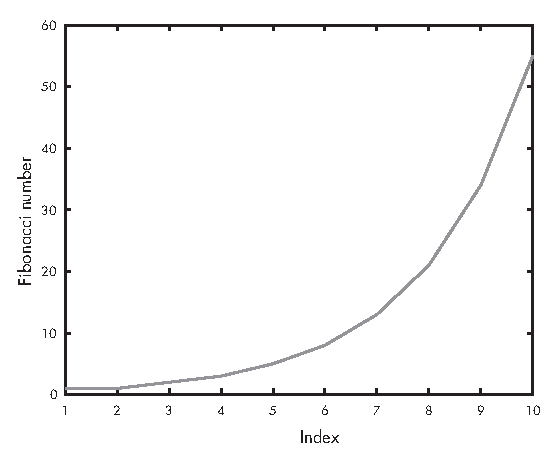
\includegraphics{images/figure04_01_new_v1.eps}
\caption{The first 10 elements of the Fibonacci sequence}
\label{fig:fibonacci}
\end{figure}

This way of looking at a vector is often useful for debugging, especially
if it is big enough that displaying the elements on
the screen is unwieldy.


\section{Common Vector Operations}

We've covered some of the basic features of vectors. Let's now look at some common patterns we use to work with data stored in vectors.

\subsection{Reduce}
\label{reduce}

We frequently use loops to run through the elements of a vector
and add them up, multiply them together, compute the sum
of their squares, and so on.  This kind of operation is called \emph{reduce},
because it reduces a vector with multiple elements down to a single
number.

\index{reduce}
\index{vector}

For example, the loop in Listing~\ref{lst:vec_reduce} adds up the elements of a vector named \lstinline{X} (which we assume has been defined).

\begin{lstlisting}[caption={Reducing a vector to a single scalar value (the sum)}, label={lst:vec_reduce}]
total = 0
for i=1:length(X)
    total = total + X(i)
end
ans = total
\end{lstlisting}

The use of \lstinline{total} as an accumulator is similar to what we
saw in Chapter~3.  Again, we use the \lstinline{length} function
to find the upper bound of the range, so this loop will work
regardless of the length of \lstinline{X}.
Each time through the loop, we add
in the \lstinline{i}th element of \lstinline{X}, so at the end of the loop
\lstinline{total} contains the sum of the elements.

\index{accumulator}
\index{length function@\lstinline{length} function}

MATLAB provides functions that perform some reduce operations.
For example, the \lstinline{sum} function computes the sum of the elements
in a vector, and \lstinline{prod} computes the product.


\subsection{Apply}
\label{apply}

Another common use of a loop is to run through the elements of
a vector, perform some operation on the elements, and create
a new vector with the results.  This operation is called
\emph{apply}, because you apply the operation to each element in
the vector.

\index{apply}

For example, the loop in Listing~\ref{lst:vec_apply} creates a vector \lstinline{Y} that
contains the squares of the elements of \lstinline{X} (assuming, again, that \lstinline{X} is already defined).

\begin{lstlisting}[caption={Making a new vector Y by squaring the elements in X}, label={lst:vec_apply}]
for i=1:length(X)
    Y(i) = X(i)^2
end
\end{lstlisting}

Many apply operations can be done with element-wise operators.
The following statement is more concise than the loop in
Listing~\ref{lst:vec_apply}.

\begin{code}
Y = X .^ 2
\end{code}

It also runs faster!


\section{Chapter Review}

In this chapter, we used a vector to store the elements of a sequence.  We learned how to select elements from a vector and perform vector arithmetic.  We performed reduce and apply operations using \lstinline{for} loops, MATLAB functions, and element-wise operations.

Here are some terms from this chapter you might want to remember.

% A {\em compound statement} is a statement, like \lstinline{if} and \lstinline{for}, that
% contains other statements in an indented body.
% If you put one compound statement in the body of another, they are {\em nested}.

% A {\em scalar} is single value; a
A \emph{vector} is a sequence of values, which is a kind of \emph{matrix}, also called an \emph{array} in some MATLAB documentation.

An \emph{index} is an integer value used to indicate one of the elements
in a vector or matrix (also called a \emph{subscript} in some MATLAB documentation).

An operation is \emph{element-wise} if it acts on the individual elements of a vector or matrix (unlike some linear algebra operations).

% You can {\em search} a vector for an element that has some desired property.
You can \emph{apply} an operation to all elements of a vector, and you can \mbox{\emph{reduce}} a vector to a single value, for example by computing the sum of the elements.

% A {\em name collision} is a scenario where two scripts that use the same variable name interfere with each other.

In the next chapter, we'll meet the most important idea in computer programming: functions!



\section{Exercises}

Before you go on, you might want to work on the following exercises.

\subsection{Exercise~1}
Write a loop that computes the first $n$ elements
of the geometric sequence $A_{i+1} = A_i/2$ with $A_1 = 1$.  Notice that
math notation puts $A_{i+1}$ on the left side of the equality.
When you translate to MATLAB, you might want to rewrite it with
$A_{i}$ on the left side.


\subsection{Exercise~2}
Write an expression that computes the square root of the sum of the squares of the elements of a vector, without using a loop.

\index{square root}


\subsection{Exercise~3}
\label{fibratio}

The ratio of consecutive Fibonacci numbers, $F_{n+1}/F_{n}$, converges
to a constant value as $n$ increases.  Write a script that computes
a vector with the first $n$ elements of a Fibonacci sequence (assuming
that the variable \lstinline{n} is defined) and then computes a new
vector that contains the ratios of consecutive Fibonacci numbers.
Plot this vector to see if it seems to converge.  What value does
it converge on?

\index{Fibonacci}

% fibonacci4.m


\subsection{Exercise~4}
  The following set of equations is based on a famous example of a chaotic system, the Lorenz attractor (see \url{https://greenteapress.com/matlab/lorenz}):
%
\begin{eqnarray*}
x_{i+1} &=& x_i + \sigma \left( y_i - x_i \right) dt  \\
y_{i+1} &=& y_i + \left[ x_i (r - z_i) - y_i \right] dt   \\
z_{i+1} &=& z_i + \left( x_i y_i - b z_i \right) dt
\end{eqnarray*}
%
\begin{enumerate}

\item Write a script that computes the first 10 elements of the sequences
$X$, $Y$, and $Z$ and stores them in vectors named \textbf{\lstinline{X}}, \textbf{\lstinline{Y}},
and \textbf{\lstinline{Z}}.

Use the initial values $X_1 = 1$, $Y_1 = 2$, and $Z_1 = 3$ with the values
$\sigma = 10$, $b = 8/3$, $r = 28$, and $dt = 0.01$.

\item Read the documentation for \lstinline{plot3} and \lstinline{comet3}, and
plot the results in three dimensions.

\item Once the code is working, use semicolons to suppress the output
and then run the program with sequence lengths of 100, 1,000, and 10,000.

\item Run the program again with different starting conditions.
What effect does it have on the result?

\item Run the program with different values for $\sigma$, $b$, and $r$,
and see if you can get a sense of how each variable affects the
system.

\end{enumerate}

\index{Lorenz attractor}
% lorenz.m



\subsection{Exercise~5}
The logistic map (see \url{https://greenteapress.com/matlab/logistic}) is described by the following equation:

\index{logistic map}

\begin{equation*}
X_{i+1} = r X_i (1-X_i)
\end{equation*}
where $X_i$ is a number between 0 and 1, and $r$ is a positive number.

\begin{enumerate}

\item Write a script named \emph{logmap.m} that computes the first 50
elements of $X$ with \lstinline{r} = 3.9 and \lstinline{X1} = 0.5, where
\lstinline{r} is the parameter of the logistic map and \lstinline{X1} is the
initial value.

\item Plot the results for a range of values of $r$ from 2.4 to 4.0.
How does the behavior of the system change as you vary $r$?

\end{enumerate}

% logmap.m






\chapter{Functions}
\label{functions}

This chapter introduces the most important idea in computer programming: functions! 
To explain why functions are so important, I'll start by explaining one of the problems they solve: name collisions.

\index{function}

\section{Name Collisions}
\label{collision}

\index{name collision}
\index{collision!name}
\index{workspace}

All scripts run in the same workspace, so if one script changes the value of a variable, all other scripts see the change.  With a small number of simple scripts, that's not a problem, but eventually the interactions between scripts become unmanageable.

For example, the following (increasingly familiar) script computes the
sum of the first {\tt n} terms in a geometric sequence, but it also
has the {\em side-effect} of assigning values to {\tt A1}, {\tt total},
{\tt i}, and {\tt a}.

\begin{code}
A1 = 1;
total = 0;
for i=1:10
    a = A1 * 0.5^(i-1);
    total = total + a;
end
ans = total
\end{code}

If you were using any of those variable names before calling this
script, you might be surprised to find, after running the script,
that their values had changed.  If you have two scripts that use
the same variable names, you might find that they work separately
and then break when you try to combine them.  This kind of
interaction is called a \emph{name collision}.

\index{script}

As the number of scripts you write increases, and they get longer
and more complex, name collisions become more of a problem.  Avoiding
this problem is one of several motivations for functions.

\section{Defining Functions}

A {\em function} is like a script, except that each function has its own workspace, so any variables defined
inside a function only exist while the function is running, and don't
interfere with variables in other workspaces, even if they have the
same name. 
Function inputs and outputs are defined carefully to avoid
unexpected interactions.

To define a new function, you create an M-file with the name you
want, and put a function definition in it.  For example, to create
a function named {\tt myfunc}, create an M-file named {\em myfunc.m}
and put the following definition into it:

\index{M-file}
\index{script}
\index{function definition}

\begin{lstlisting}[caption={A function definition}, label={lst:function_def}]
function res = myfunc(x)
    s = sin(x)
    c = cos(x)
    res = abs(s) + abs(c)
end
\end{lstlisting}

The first non-comment word of the file has to be {\tt function}, because
that's how MATLAB tells the difference between a script and a function
file.

\index{compound statement}
\index{definition!function}

A function definition is a compound statement.  The first line
is called the {\em signature} of the function; it defines
the inputs and outputs of the function.  In Listing~\ref{lst:function_def} the {\em input variable} is named {\tt x}.  When this function is called, the
argument provided by the user will be assigned to {\tt x}.

\index{input variable}
\index{variable!input}

\index{output variable}
\index{variable!output}

The {\em output variable} is named {\tt res}, which is short for
``result''.  You can call the output variable whatever you want, but
as a convention, I like to call it {\tt res}.  Usually the last
thing a function does is assign a value to the output variable.

\index{res@{\tt res}}
\index{ans@{\tt ans}}

Once you've defined a new function, you call it the same way you
call built-in MATLAB functions.  If you call the function as a statement,
MATLAB puts the result into {\tt ans}:

\begin{code}
>> ***myfunc(1)***

s = 0.84147098480790

c = 0.54030230586814

res = 1.38177329067604

ans = 1.38177329067604
\end{code}

But it's more common (and better style) to assign the result to
a variable:

\begin{code}
>> ***y = myfunc(1)***

s = 0.84147098480790

c = 0.54030230586814

res = 1.38177329067604

y = 1.38177329067604
\end{code}

While you're debugging a new function, you might want to display
intermediate results like this, but once it's working, you'll want
to add semi-colons to make it a {\em silent function}.  A silent function
computes a result but doesn't display
anything (except sometimes warning messages). Most built-in
functions are silent.

\index{silent function}
\index{function!silent}
\index{workspace}

Each function has its own workspace, which is created when the
function starts and destroyed when the function ends.  If you try to
access (read or write) the variables defined inside a function, you
will find that they don't exist.

\begin{code}
>> ***clear***
>> ***y = myfunc(1);***
>> ***who***
Your variables are: y

>> ***s***
Undefined function or variable 's'.
\end{code}

The only value from the function that you can access is the result,
which in this case is assigned to {\tt y}.

If you have variables named {\tt s} or {\tt c} in your workspace
before you call {\tt myfunc}, they will still be there when the
function completes.

\begin{code}
>> ***s = 1;***
>> ***c = 1;***
>> ***y = myfunc(1);***
>> ***s, c***

s = 1
c = 1
\end{code}

So inside a function you can use whatever variable names you
want without worrying about collisions.

\index{name collision}
\index{collision!name}


\section{Function Documentation}

\index{documentation}
\index{comment}

At the beginning of every function file, you should include a comment
that explains what the function does:

\index{Documentation!functions}

\begin{code}
% res = myfunc(x)
% Compute the Manhattan distance from the origin to the
% point on the unit circle with angle (x) in radians.

function res = myfunc(x)
% this is not part of documentation given by help function

    s = sin(x);
    c = cos(x);
    res = abs(s) + abs(c);
end
\end{code}

When you ask for {\tt help}, MATLAB prints the comment you provide.

\index{help@{\tt help}}

\begin{code}
>> ***help myfunc***
  res = myfunc(x)
  Compute the Manhattan distance from the origin to the
  point on the unit circle with angle (x) in radians.
\end{code}

There are lots of conventions about what should be included
in these comments.  Among other things, it's a good idea to
include

\begin{description}

\item [Signature:] The signature of the function, which includes the name
of the function, the input variable(s) and the output variable(s).

\item [Description:] A clear, concise, abstract description of what the function does.
An {\em abstract} description is one that leaves out the
details of {\em how} the function works, and includes only information
that someone using the function needs to know.  You can put additional
comments inside the function that explain the details.

\item [Variables:] An explanation of what the input variables mean; for example,
in this case it is important to note that {\tt x} is considered
to be an angle in radians.

\item [Conditions:] Any preconditions and postconditions.

\end{description}

\index{precondition}
\index{postcondition}

\section{Naming Functions}
\index{Functions!naming}

There are a few ``gotchas'' that come up when you start defining functions.
The first is that the ``real'' name of your function is determined by the file name, {\em not} by the name you put in the function signature.  As a matter of style, you
should make sure that they are always the same, but if you
make a mistake, or if you change the name of a function, it's
easy to get confused.

\index{function name}
\index{name!function}

In the spirit of making errors on purpose, change the name of
the function in \verb"myfunc" to \verb"something_else", and
then run it again.

If this is what you put in \emph{myfunc.m}:

\begin{code}
function res = something_else (x)
    s = sin(x);
    c = cos(x);
    res = abs(s) + abs(c);
end
\end{code}

Here's what you'll get:

\begin{code}
>> ***y = myfunc(1)***
y = 1.3818

>> ***y = something_else(1)***
Undefined function or variable 'something_else'.
\end{code}

{\tt myfunc} still works because that's the name of the file.
\verb"something_else" doesn't work because the name of the function is ignored.

The second gotcha is that the name of the file can't have spaces.
For example, if you write a function and rename the file to 
{\em my func.m},
and then try to run it, you get:

\begin{code}
>> ***y = my func(1)***
 y = my func(1)
        |
Error: Unexpected MATLAB expression.
\end{code}

This fails because MATLAB thinks \verb"my" and \verb"func" are two different
variable names.

The third gotcha is that your function names can collide with built-in
MATLAB functions.  For example, if you create an M-file named {\em sum.m}, and then call {\tt sum}, MATLAB might call {\em your} new
function, not the built-in version!  Which one actually gets called
depends on the order of the directories in the search path, and
(in some cases) on the arguments.  As an example, put the following
code in a file named {\em sum.m}:

\index{name collision}
\index{collision!name}

\begin{code}
function res = sum(x)
   res = 7;
end
\end{code}

And then try this:

\begin{code}
>> ***sum(1:3)***

ans = 6

>> ***sum***

ans = 7
\end{code}

In the first case MATLAB used the built-in function; in the second
case it ran your function!  This kind of interaction can be very
confusing.  Before you create a new function, check to see if there is
already a MATLAB function with the same name.  If there is, choose
another name!

\section{Multiple Input Variables}
\label{hypotenuse}

\index{input variable}
\index{variable!input}

Functions can take more than one input variable.
For example, the following function takes two input variables,
{\tt a} and {\tt b}:

\begin{lstlisting}[caption={A function that computes the sum of squares of two numbers}, label={lst:hyp_function}]
function res = sum_squares(a, b)
    res = a^2 + b^2;
end
\end{lstlisting}
  
This function computes the sum of squares of two numbers, {\tt a}
and {\tt b}.

If we call it from the Command Window with arguments 3 and 4, we can
confirm that the sum of their squares is 25.

\begin{code}
>> ***ss = sum_squares(3, 4)***
ss = 25
\end{code}

The arguments you provide are assigned to the input variables in
order, so in this case 3 is assigned to {\tt a} and 4 is assigned to
{\tt b}.  MATLAB checks that you provide the right number of arguments;
if you provide too few, you get

\begin{code}
>> ***ss = sum_squares(3)***
Not enough input arguments.

Error in sum_squares (line 4)
    res = a^2 + b^2;
\end{code}

This error message might be confusing, because it suggests that
the problem is in \verb"sum_squares" rather than in the function call.
Keep that in mind when you're debugging.

If you provide too many arguments, you get

\begin{code}
ss = sum_squares(3, 4, 5)
Error using sum_squares
Too many input arguments.
\end{code}

That's a better error message, because it's clear that the problem isn't in the function; it's in the way we're using the function.

\section{Summary}

Now that we know about functions, and all the ways they can go wrong, let's put them to good use.  In the next chapter we'll develop a program that uses several functions to search for Pythagorean triples (and I'll explain what those are).

Here are a few terms in this chapter you might want to remember:

A function is a named sequence of statements stored in an M-file.
A function can have one or more input variables, which get their values when the function is called, and output variables, which return a value from the function to the caller.

The first line of a function definition is its ``signature'', which
specifies the name of the function, the input variables, and the
output variables.

A ``silent function'' doesn't display anything, generate a figure, or have any other effect other than returning output values.


\section{Exercises}

\begin{ex}
\label{hypotenuse_exercise}
Write a function called {\tt hypotenuse} that takes two parameters, {\tt a} and {\tt b}, that represent the lengths of two sides of a right triangle.  It should assign to {\tt res} the length of the third side of the triangle, given by the formula:

\[ c = \sqrt{a^2 + b^2} \]
\end{ex}


\chapter{Conditionals}


In this chapter, we'll use functions and a new feature---conditional statements---to search for Pythagorean triples.
A Pytha\-gorean triple is a set of integers, like~3, 4, and 5,
that are the lengths of the sides of a right triangle.  Mathematically, it's a set of integers $a$, $b$, and $c$ such that $a^2 + b^2 = c^2$.
This example will also demonstrate the \emph{incremental development} process we talked about in Chapter~\ref{loops}.

\index{Pythagorean triple}

\section{Relational Operators}
\index{operator!relational}

Suppose we have three variables, \lstinline{a}, \lstinline{b}, and \lstinline{c}, and we want to check whether they form a Pythagorean triple.  We can use the equality operator (\lstinline{==}) to compare two values:

\begin{code}
>> a = 3;
>> b = 4;
>> c = 5;
(*\pagebreak*)
>> a^2 + b^2 == c^2

ans = logical 1
\end{code}

The result is a \emph{logical} value, which means it's either~\lstinline{1}, which means ``true,'' or~\lstinline{0}, which means ``false.''  Here's an example where the result is false:

\begin{code}
>> c = 6;
>> a^2 + b^2 == c^2
ans = logical 0
\end{code}

It's a common error to use the assignment operator (\lstinline{=}) instead of the equality operator (\lstinline{==}).  If you do, you get an error:

\begin{code}
>> a^2 + b^2 = c^2
 a^2 + b^2 = c^2
           |
Error: Incorrect use of '=' operator.
To assign a value to a variable, use '='.
To compare values for equality, use '=='.
\end{code}

The equality operator is one of several \emph{relational operators}, so called because they test relations between values.
For example, \lstinline{x < 10} is true (\lstinline{1}) if the value of \lstinline{x} is less than \lstinline{10} or false (\lstinline{0}) if otherwise.  And \lstinline{x > 0} is true if \lstinline{x} is greater than~\lstinline{0}.

The other relational operators are \lstinline{<=} for ``less or equal,'' \lstinline{>=} for ``greater or equal,'' and  \lstinline{~=} for ``not equal.''


\section{if Statement}

\index{if statement@\lstinline{if} statement}
\index{conditional statement}

Now suppose that when we find a Pythagorean triple we want to display a message.
The \lstinline{if} statement allows you to check for certain conditions
and execute statements if the conditions are met.  For example:

\begin{code}
if a^2 + b^2 == c^2
    disp("Yes, that is a Pythagorean triple.")
end
\end{code}

The syntax is similar to a \lstinline{for} loop.  The first line
specifies the condition we're interested in.  If the condition is true,
MATLAB executes the \emph{body} of the statement, which is the indented sequence of
statements between the \lstinline{if} and the \lstinline{end}.

\index{indentation}

MATLAB doesn't require you to indent the body of an \lstinline{if}
statement, but it makes your code more readable, so you should do it.

If the condition is not satisfied, the statements in the body are
not \mbox{executed}.

Sometimes there are alternative statements to
execute when the condition is false.  In that case, you can extend
the \lstinline{if} statement with an \lstinline{else} clause.

\index{else clause@\lstinline{else} clause}

The complete version of the previous example might look like this:

\begin{code}
if a^2 + b^2 == c^2
    disp("Yes, that is a Pythagorean triple.")
else
    disp("No, that is not a Pythagorean triple.")
end
\end{code}

Statements like \lstinline{if} and \lstinline{for} that contain other statements
are called \emph{compound} statements.  All compound statements finish
with \lstinline{end}.

\index{compound statement}
\index{statement!compound}



\section{Incremental Development}
\label{increxample}
\index{incremental development}

Now that we have relational operators and \lstinline{if} statements, let's start writing
the program.

Here are the steps we will follow to develop the program incrementally:

\begin{enumerate}

\item Encapsulate the \lstinline{if} statement from the previous section in a function called \lstinline{is_pythagorean}.

\item Write a script named \emph{find\textunderscore triples.m} and start with a loop that enumerates values of \lstinline{a} and displays them.

\item Write a second loop that enumerates values of \lstinline{b} and a third loop that enumerates values of \lstinline{c}.

\item Use \lstinline{is_pythagorean} to check whether \lstinline{a}, \lstinline{b}, and \lstinline{c} form a Pythagorean triple.

\item Use an \lstinline{if} statement to display only values that pass the test.

\item Transform the script into a function and make it take an input variable that specifies the range to search.

\end{enumerate}

Along the way, we'll optimize the program to eliminate unnecessary work.


\section{Logical Functions}

The first step is to create a \emph{logical function}, which is a function that returns a logical value.
The following function takes three input variables, \lstinline{a}, \lstinline{b}, and~\lstinline{c}, and returns true (\lstinline{1}) if they form a Pythagorean triple and false (\lstinline{0}) otherwise.

\begin{code}
function res = is_pythagorean(a, b, c)
    if a^2 + b^2 == c^2
        res = 1;
    else
        res = 0;
    end
end
\end{code}

We can use this function like so:


\begin{code}
>> is_pythagorean(3, 4, 5)
ans = 1
\end{code}

But we can write the same function more concisely, like this:

\begin{code}
function res = is_pythagorean(a, b, c)
    res = a^2 + b^2 == c^2;
end
\end{code}

The result of the equality operator is a logical value, which we can assign directly
to \lstinline{res}.

Put this function in a file called \emph{is\_pythagorean.m}, so we can use it as part of our program.


\section{Nested Loops}

The next step is to write loops that enumerate different values of \lstinline{a}, \lstinline{b}, and
\lstinline{c}.  Create a new file called \emph{find\_triples.m} where we'll develop the rest of the program.

\index{nested loop}
\index{loop!nested}

We'll start with a loop for \lstinline{a}:

\begin{code}
for a=1:3
    a
end
\end{code}

It might seem silly to start with such a simple program, but this is an essential element of incremental development: start simple and test as you go.

The output is as expected.

\begin{code}
1
2
3
\end{code}

Now we'll add a second loop for \lstinline{b}.  It might be tempting to write something like this:

\begin{code}
for a=1:3
    disp(a)
end
for b=1:4
    disp(b)
end
\end{code}

But that loops through the values of \lstinline{a} and then loops through the values of \lstinline{b}, and that's not what we want.

Instead, we want to consider every possible pair of values, like this:

\begin{code}
for a=1:3
    for b=1:4
        disp([a,b])
    end
end
\end{code}

Now one loop is inside the other.  The inner loop gets executed three times, once for each value of \lstinline{a}, so here's what the output looks like (I've adjusted the spacing to make the structure clear):

\begin{code}
>> find_triples
     1     1
     1     2
     1     3
     1     4
     2     1
     2     2
     2     3
     2     4
     3     1
     3     2
     3     3
     3     4
\end{code}

The left column shows the values of \lstinline{a} and the right column shows the values of \lstinline{b}.

The next step is to search for values of \lstinline{c} that might make a Pythagorean triple.  The largest possible value for \lstinline{c} is \lstinline{a + b}, because otherwise we couldn't form a triangle
(see \url{https://greenteapress.com/matlab/triangle}).

\begin{code}
for a=1:3
    for b=1:4
        for c=1:a+b
            disp([a,b,c])
        end
    end
end
\end{code}

After each small change, run the program again and check the output.

\section{Putting It Together}

Now instead of displaying all of the triples, we'll add an \lstinline{if} statement and display only Pythagorean triples:

\begin{code}
for a=1:3
    for b=1:4
        for c=1:a+b
            if is_pythagorean(a, b, c)
                disp([a,b,c])
            end
        end
    end
end
\end{code}

The result is just one triple:

\begin{code}
>> find_triples
     3     4     5
\end{code}

You might notice that we're wasting some effort here.
After checking the case when \lstinline{a} is~1 and \lstinline{b} is~2, there's no point in checking
the case when \lstinline{a} is~2 and \lstinline{b} is~1.  We can save the extra work by adjusting the
range of \lstinline{b}:

\begin{code}
for b=a:4
\end{code}

We can save even more work by adjusting the range of \lstinline{c}:

\begin{code}
for c=b:a+b
\end{code}

Here's the final version:

\begin{code}
for a=1:3
    for b=a:4
        for c=b:a+b
            if is_pythagorean(a, b, c)
                disp([a,b,c])
            end
        end
    end
end
\end{code}

\section{Encapsulation and Generalization}

As a script, this program has the side effect of assigning values to
\lstinline{a}, \lstinline{b}, and \lstinline{c}, which would be bad if any of those names were in use.
By wrapping the code in a function, we can avoid name collisions; this process is called \emph{encapsulation} because it isolates this program from the workspace.

\index{encapsulation}
\index{generalization}

The first draft of the function takes no input variables:

\begin{code}
function res = find_triples()
    for a=1:3
        for b=a:4
            for c=b:a+b
                if is_pythagorean(a, b, c)
                    disp([a,b,c])
                end
            end
        end
    end
end
\end{code}

The empty parentheses in the signature are not necessary, but
they make it apparent that there are no input variables.  Similarly,
it's a good  idea when calling the new function to use parentheses as a reminder
that it's a function, not a script:

\begin{code}
>> find_triples()
\end{code}

The output variable isn't necessary, either; it
never gets assigned a value.  But I put it there as a matter of
habit and so my function signatures all have the same structure.

\index{output variable}
\index{variable!output}

The next step is to generalize this function by adding input
variables.  The natural generalization is to replace the constant
values~\lstinline{3} and~\lstinline{4} with a variable so we can search an arbitrarily large
range of values.

\begin{code}
function res = find_triples(n)
    for a=1:n
        for b=a:n
            for c=b:a+b
                if is_pythagorean(a, b, c)
                    disp([a,b,c])
                end
            end
        end
    end
end
\end{code}

Here are the results for the range from 1 to 15:

\begin{code}
>> find_triples(15)
     3     4     5
     5    12    13
     6     8    10
     8    15    17
     9    12    15
\end{code}

The triples $5,12,13$ and $8,15,17$ are new, but the others are just multiples of the $3,4,5$ triangle.

\section{Adding a continue Statement}

\index{continue@\lstinline{continue}}

As a final improvement, let's modify the function so it only
displays the ``lowest'' of each Pythagorean triple, and not the
multiples.

The simplest way to eliminate the multiples is to check whether
\lstinline{a} and \lstinline{b} share a common factor.  If they do, dividing both
by the common factor yields a smaller, similar triangle that has
already been checked.

\index{gcd function@\lstinline{gcd} function}
\index{function!gcd@\lstinline{gcd}}

MATLAB provides a \lstinline{gcd} function that computes the greatest common
divisor of two numbers.  If \lstinline{gcd(a,b)} is greater than 1,
\lstinline{a} and \lstinline{b} share a common factor and we can use the \lstinline{continue}
statement to skip to the next pair. Listing~\ref{lst:triples_function} contains the final version of this function:

\begin{lstlisting}[caption={Our final Pythagorean triples function}, label={lst:triples_function}]
function res = find_triples(n)
    for a=1:n
        for b=a:n
            for c=b:a+b
                if gcd(a,b) > 1
	                continue
                end
                if is_pythagorean(a, b, c)
                    disp([a,b,c])
                end
            end
        end
    end
end
\end{lstlisting}

The \lstinline{continue} statement  causes the program to end the current iteration
immediately, jump to the top of the loop, and ``continue'' with the next iteration.

In this case, since there are three loops, it might not be obvious which loop to jump to, but the rule is to jump to the innermost loop (which is what we want).

Here are the results with \lstinline{n = 40}:

\begin{code}
>> find_triples(40)
     3     4     5
     5    12    13
     7    24    25
     8    15    17
     9    40    41
    12    35    37
    20    21    29
\end{code}


\section{How Functions Work}
\index{function}

Let's review the sequence of steps that occur when you call a function:

\begin{enumerate}

\item Before the function starts running, MATLAB creates a new
workspace for it.
\index{workspace}

\item MATLAB evaluates each of the arguments and assigns
the resulting values, in order, to the input variables (which
live in the \emph{new} workspace).

\item The body of the code executes.  Somewhere in the body
a value gets assigned to the output variable.

\item The function's workspace is destroyed; the only thing
that remains is the value of the output variable and any side
effects the function had (like displaying values).

\item The program resumes from where it left off.  The value
of the function call is the value of the output variable.

\end{enumerate}

When you're reading a program and you come to a function call,
there are two ways to interpret it. You can think about the mechanism I just described,
and follow the execution of the program into the function and back, or you can assume that the function works correctly, and go on to the next statement after the function call.

When you use a built-in function, it's natural to assume that it works, in part because you don't
usually have access to the code in the body of the function.
But when you start writing your own functions, you might
find yourself following the ``flow of execution.''  This can
be useful while you are learning, but as you gain experience, you
should get more comfortable with the idea of writing a function,
testing it to make sure it works, and then forgetting about the
details of how it works.

\index{flow of execution}
\index{abstraction}

Forgetting about details is called \emph{abstraction}; in the context
of functions, abstraction means forgetting about \emph{how} a function
works and just assuming (after appropriate testing) that it works.
For many people, it takes some time to get comfortable with functions.  If you are one of them, you might be tempted to avoid functions, and sometimes you can get by without them.

But experienced programmers use functions extensively, for several good reasons. First, each function has its own workspace, so using functions helps
avoid name collisions.
Functions also lend themselves to incremental development: you can
debug the body of the function first (as a script), then encapsulate
it as a function, and then generalize it by adding input variables.

Also, functions allow you to divide a large problem into small
pieces, work on the pieces one at a time, and then assemble a
complete solution.

Once you have a function working, you can forget about the
details of how it works and concentrate on what it does.  This
process of abstraction is an important tool for managing the
complexity of large programs.


\section{Chapter Review}

In this chapter, we encountered relational operators and \lstinline{if} statements, and we used them to develop a program that searches for Pythagorean triples.
We wrote a \emph{logical function}, which is a function that returns a logical value
(\lstinline{1} for ``true'' or \lstinline{0}~for ``false'').

We also saw an example of \emph{incremental development}, or developing programs gradually, adding just a few lines of code at a time and testing as you go.  If you develop programs this way, you will have fewer bugs and you will find them more quickly.

This chapter defined two new terms: \emph{encapsulation} is the process of wrapping part of a program in
a function in order to limit interactions (including name collisions)
between the function and the rest of the program; \emph{abstraction} is the process of ignoring the details of how a function works in order to focus on a simpler model of what the
function does.

The next chapter introduces a new tool, called \lstinline{fzero}, that we'll use to solve nonlinear equations.


\section{Exercise}

Before you go on, you might want to work on the following exercise.

\begin{ex}
\index{Fibonacci number}
\index{Pythagorean triple}

There is an interesting connection between Fibonacci numbers and
Pythagorean triples.  If $F$ is a Fibonacci sequence, then

\begin{equation*}
\big(F_i F_{i+3}, \, 2 F_{i+1} F_{i+2}, \, F_{i+1}^2 + F_{i+2}^2 \big)
\end{equation*}
is a Pythagorean triple, for all $i \ge 1$.

Write a function named \lstinline{fib_triple} that
takes \lstinline{n} as an input variable, computes
the first \lstinline{n} Fibonacci numbers, stores them in a vector,
and checks whether this formula produces Pythagorean triples for numbers in the \mbox{sequence}.

% fib_triple.m

\end{ex}


\documentclass[main.tex]{subfiles}

\begin{document}

\chapter{Functions of Vectors}

Now that we have functions and vectors, we'll put them together to write functions that take vectors as input variables and return vectors as output variables.  And you'll see two patterns for computing with vectors, existential and universal quantification.  But first, let's talk about organizing functions and files.

\section{Functions and files}
\label{funfiles}

So far we have only put one function in each file.  It is also possible
to put more than one function in a file, but only the first one, the
{\bf top-level function}, can be called from the {\sf Command
Window}. 
The other {\bf helper functions} can be called from anywhere inside the file, but not from any other file.

\index{function!top-level}
\index{top-level function}

Large programs almost always require more than one function; keeping
multiple functions in one file is convenient, but it makes debugging
difficult because you can't call helper functions from the {\sf Command
Window}.

\index{helper function}
\index{function!helper}

To help with this problem, I often use the top-level function
to develop and test my helper functions.  For example, to write
a program for Exercise~\ref{duck}, I would create a file named
{\tt duck.m} and start with a top-level function named {\tt duck}
that takes no input variables and returns no output value.

Then I would write a function named {\tt error\_func} to
evaluate the error function for {\tt fzero}.  To test
{\tt error\_func} I would call it from {\tt duck} and then
call {\tt duck} from the {\sf Command Window}.

\index{incremental development}

Here's what my first draft might look like:

\begin{code}
function res = duck()
    error = error_func(10)
end

function res = error_func(d)
    rho = 0.3;      % density in g / cm^3
    r = 10;         % radius in cm
    res = d;
end
\end{code}

The line {\tt res = d} isn't finished yet, but this
is enough code to test.
Once I finished and tested {\tt error\_func}, I would modify
{\tt duck} to use {\tt fzero}.

For this problem we might only need two functions, but if there
were more, I could write and test them one at a time, and then
combine them into a working program.


\section{Vectors as input variables}

Since many of the built-in functions take vectors as arguments,
it should come as no surprise that you can write functions that
take vectors.  Here's a simple (silly) example:

\index{vector}
\index{input variable}

\begin{code}
function res = display_vector(X)
    X
end
\end{code}

There's nothing special about this function at.  The only
difference from the scalar functions we've seen is that I used
a capital letter to remind me that {\tt X} is a vector.

This is another example of a function that doesn't actually return a value; it just displays the value of the input variable:

\begin{code}
>> display_vector(1:3)
X = 1     2     3
\end{code}

Here's a more interesting example that encapsulates the code
from Section~\ref{reduce} that adds up the elements of a vector:

\index{encapsulation}

\begin{code}
function res = mysum(X)
    total = 0;
    for i=1:length(X)
        total = total + X(i);
    end
    res = total;
end
\end{code}

I called it {\tt mysum} to avoid a collision with the built-in
function {\tt sum}, which does pretty much the same thing.

\index{sum@{\tt sum}}

Here's how you call it from the {\sf Command Window}:

\begin{code}
>> total = mysum(1:3)
total = 6
\end{code}

Because this function has an output variable, I made a
point of assigning it to a variable.

\index{output variable}


\section{Vectors as output variables}

There's also nothing wrong with assigning a vector to an output
variable.  Here's an example that encapsulates the code from
Section~\ref{apply}:

\begin{code}
function res = myapply(X)
    for i=1:length(X)
        Y(i) = X(i)^2;
    end
    res = Y;
end
\end{code}

Here's how {\tt myapply} works:
\index{apply}

\begin{code}
>> V = myapply(1:3)
V = 1     4     9
\end{code}

\begin{ex}
Write a function named {\tt myfind} that
encapsulates the code, from Section~\ref{search}, that finds the
location of a target value in a vector.
\end{ex}



\section{Vectorizing functions}

Functions that work on vectors will almost always work on scalars
as well, because MATLAB considers a scalar to be a vector with
length 1.

\index{vectorizing}
\index{function!vectorizing}

\begin{code}
>> mysum(17)
ans = 17

>> myapply(9)
ans = 81
\end{code}

Unfortunately, the converse is not always true.  If you write
a function with scalar inputs in mind, it might not work on vectors.

But it might!  If the operators and functions
you use in the body of your function work on vectors, then your
function will probably work on vectors.

For example, here is the very first function we wrote:

\begin{code}
function res = myfunc(x)
    s = sin(x);
    c = cos(x);
    res = abs(s) + abs(c);
end
\end{code}

And lo!  It turns out to work on vectors:

\begin{code}
>> Y = myfunc(1:3)
Y = 1.3818    1.3254    1.1311
\end{code}

Some of the other functions we wrote don't work on vectors,
but they can be patched up with just a little effort.  For example,
here's {\tt hypotenuse} from Section~\ref{hypotenuse}:

\begin{code}
function res = hypotenuse(a, b)
    res = sqrt(a^2 + b^2);
end
\end{code}

This doesn't work on vectors because the \verb+^+ operator
tries to do matrix exponentiation, which only works on
square matrices.

\index{matrix exponentiation}

\begin{code}
>> hypotenuse(1:3, 1:3)
Error using  ^  (line 51)
Incorrect dimensions for raising a matrix to a power. 
Check that the matrix is square and the power is a scalar. 
To perform elementwise matrix powers, use '.^'.
\end{code}

But if you replace \verb+^+ with the elementwise operator
\verb+.^+, it works!

\index{elementwise operator}

\begin{code}
>> A = [3,5,8];
>> B = [4,12,15];
>> C = hypotenuse(A, B)

C = 5    13    17
\end{code}

The function matches up corresponding elements from the two
input vectors, so the elements of {\tt C} are the hypotenuses of
the pairs $(3,4)$, $(5,12)$, and $(8,15)$, respectively.

In general, if you write a function using only elementwise
operators and functions that work on vectors, the new
function will also work on vectors.


\section{Sums and differences}

Another common vector operation is {\bf cumulative sum}, which takes a
vector as an input and computes a new vector that contains all of the
partial sums of the original.  In math notation, if $V$ is the
original vector, then the elements of the cumulative sum, $C$, are:

\index{cumulative sum}
\index{sum!cumulative}

\begin{equation}
C_i = \sum_{j=1}^i V_j
\end{equation}

In other words, the $i$th element of $C$ is the sum of the first
$i$ elements from $V$.  MATLAB provides a function named {\tt cumsum}
that computes cumulative sums:

\index{cumsum@{\tt cumsum}}

\begin{code}
>> X = 1:5

X = 1     2     3     4     5

>> C = cumsum(X)

C = 1     3     6    10    15
\end{code}

The inverse operation of {\tt cumsum} is {\tt diff}, which computes
the difference between successive elements of the input vector.

\index{diff@{\tt diff}}

\begin{code}
>> D = diff(C)

D = 2     3     4     5
\end{code}

Notice that the output vector is shorter by one than the input
vector.  As a result, MATLAB's version of {\tt diff} is not
exactly the inverse of {\tt cumsum}.  If it were, then we would
expect {\tt cumsum(diff(X)} to be {\tt X}:

\begin{code}
>> cumsum(diff(X))

ans = 1     2     3     4
\end{code}

But it isn't.

\begin{ex}
Write a function named {\tt mydiff} that computes the
inverse of {\tt cumsum}, so that {\tt cumsum(mydiff(X))} and
{\tt mydiff(cumsum(X))} both return {\tt X}.

% mydiff.m
\end{ex}


\section{Products and ratios}

The multiplicative version of {\tt cumsum} is {\tt cumprod},
which computes the {\bf cumulative product}.  In math notation,
that's:

\index{cumulative product}
\index{product!cumulative}
\index{cumprod@{\tt cumprod}}

\begin{equation}
P_i = \prod_{j=1}^i V_j
\end{equation}

In MATLAB, that looks like:

\begin{code}
>> V = 1:5

V = 1     2     3     4     5

>> P = cumprod(V)

P = 1     2     6    24   120
\end{code}

MATLAB doesn't provide the multiplicative version
of {\tt diff}, which would be called {\tt ratio}, and which would
compute the ratio of successive elements of the input vector.

\begin{ex}
Write a function named {\tt myratio} that computes the
inverse of {\tt cumprod}, so that {\tt cumprod(myratio(X))} and
{\tt myratio(cumprod(X))} both
return {\tt X}.

You can use a loop, or if you want to be clever, you can take
advantage of the fact that $e^{\ln a + \ln b} = a b$.

If you apply {\tt myratio} to a vector that contains Fibonacci
numbers, you can confirm that the ratio of successive elements
converges on the golden ratio, $(1+\sqrt{5})/2$ (see
Exercise~\ref{fibratio}).

% TODO
\end{ex}



\section{Existential quantification}

\index{existential quantification}
\index{quantification!existential}

It is often useful to check the elements of a vector to see if there
are any that satisfy a condition.  For example, you might want to
know if there are any positive elements.  In logic, this condition
is called {\bf existential quantification}, and it is denoted with
the symbol $\exists$, which is pronounced ``there exists.''  For example,
this expression
%
\[ \exists x \mbox{~in~} S: x>0  \]
%
means, ``there exists some element $x$ in the set $S$ such that
$x>0$.''  In MATLAB it is natural to express this idea with a logical
function, like {\tt exists}, that returns 1 if there is such an
element and 0 if there is not.

\begin{code}
function res = exists(X)
    for i=1:length(X)
        if X(i) > 0
            res = 1;
            return
        end
    end
    res = 0;
end
\end{code}

We haven't seen the {\tt return} statement before; it is similar
to {\tt break} except that it breaks out of the whole function, not
just the loop.  That behavior is what we want here because as soon
as we find a positive element, we know the answer (it exists!) and
we can end the function immediately without looking at the rest
of the elements.

\index{return statement@{\tt return} statement}
\index{statement!{\tt return}}

If we get to the end of the loop, that means we didn't find what
we were looking for, so the result is 0.



\section{Universal quantification}

\index{universal quantification}
\index{quantification!universal}

Another common operation on vectors is to check whether {\em all}
of the elements satisfy a condition, which is known to
logicians as {\bf universal quantification}, denoted with
the symbol $\forall$, and pronounced ``for all.''  So this
expression
%
\[ \forall x \mbox{~in~} S: x>0 \]
%
means ``for all elements, $x$, in the set $S$, $x>0$.''

One way evaluate this expression in MATLAB is to
count the number of elements that satisfy the condition.
A better way is to reduce the problem to
existential quantification; that is, to rewrite

\begin{equation}
\forall x \mbox{~in~} S: x>0
\end{equation}

as

\begin{equation}
\sim \exists x \mbox{~in~} S: x \le 0
\end{equation}

Where $\sim \exists$ means ``does not exist.''
In other words, checking that all the elements are positive is
the same as checking that there are no elements
that are non-positive.

\begin{ex}
Write a function named {\tt forall} that
takes a vector and returns 1 if all of the elements are positive
and 0 if there are any non-positive elements.
\end{ex}




\section{Logical vectors}

When you apply a logical operator to a vector, the result is a 
{\bf logical vector}; that is, a vector whose elements are the logical
values 1 and 0.

\index{logical vector}
\index{vector!logical}

\begin{code}
>> V = -3:3

V = -3    -2    -1     0     1     2     3

>> L = V>0

L =  0     0     0     0     1     1     1
\end{code}

In this example, {\tt L} is a logical vector whose elements
correspond to the elements of {\tt V}.  For each positive element of
{\tt V}, the corresponding element of {\tt L} is 1.

Logical vectors can be used like flags to store the state of
a condition.  And they are often used with the {\tt find} function,
which takes a logical vector and returns a vector that contains
the indices of the elements that are ``true''.

\index{flag}
\index{find@{\tt find}}

Applying {\tt find} to {\tt L} yields

\begin{code}
>> find(L)

ans = 5     6     7
\end{code}

which indicates that elements 5, 6 and 7 have the value 1.

If there are no ``true'' elements, the result is an empty vector.

\begin{code}
>> find(V>10)

ans = Empty matrix: 1x0
\end{code}

This example computes the logical vector and passes it as an
argument to {\tt find} without assigning it to an intermediate
variable.  You can read this version abstractly as ``find
the indices of elements of {\tt V} that are greater than 10.''

We can also use {\tt find} to write {\tt exists} more concisely:

\begin{code}
function res = exists(X)
    L = find(X>0)
    res = length(L) > 0
end
\end{code}

\begin{ex}
Write a version of {\tt forall} using {\tt find}.
\end{ex}


\section{Debugging in four acts}

\index{debugging}
\index{reading}
\index{running}
\index{ruminating}
\index{retreating}

When you are debugging a program, and especially if you are working on a hard bug, there are four things to try:

\begin{description}

\item[reading:] Examine your code, read it back to yourself, and
check that it means what you meant to say.

\item[running:] Experiment by making changes and running different
versions.  Often if you display the right thing at the right place
in the program, the problem becomes obvious, but you might have to invest time building scaffolding.

\item[ruminating:] Take some time to think!  What kind of error
is it: syntax, run-time, or logical?  What information can you get from
the error messages, or from the output of the program?  What kind of
error could cause the problem you're seeing?  What did you change
last, before the problem appeared?

\item[retreating:] At some point, the best thing to do is back
off, undoing recent changes, until you get back to a program that
works, and that you understand.  Then you can starting rebuilding.

\end{description}

Beginning programmers sometimes get stuck on one of these activities
and forget the others.  Each activity comes with its own failure
mode.

For example, reading your code might help if the problem is a
typographical error, but not if the problem is a conceptual
misunderstanding.  If you don't understand what your program does, you
can read it 100 times and never see the error, because the error is in
your head.

Running experiments can help, especially if you run small, simple
tests.  But if you run experiments without thinking or reading your
code, you might fall into a pattern I call ``random walk programming,''
which is the process of making random changes until the program
does the right thing.  Needless to say, random walk programming
can take a long time.

\index{random walk programming}

The way out is to take more time to think.  Debugging is like an
experimental science.  You should have at least one hypothesis about
what the problem is.  If there are two or more possibilities, try to
think of a test that would eliminate one of them.

\index{hypothesis}

Taking a break sometimes helps with the thinking.  So does talking.
If you explain the problem to someone else (or even yourself), you
will sometimes find the answer before you finish asking the question.

But even the best debugging techniques will fail if there are too many
errors, or if the code you are trying to fix is too big and
complicated.  Sometimes the best option is to retreat, simplifying the
program until you get to something that works, and then rebuild.

Beginning programmers are often reluctant to retreat, because
they can't stand to delete a line of code (even if it's wrong).
If it makes you feel better, copy your program into another file
before you start stripping it down.  Then you can paste the pieces
back in a little bit at a time.

\index{debugging!Eighth Theorem}

To summarize, here's the Eighth Theorem of Debugging:

\begin{quote}
Finding a hard bug requires reading, running, ruminating,
and sometimes retreating.  If you get stuck on one of these
activities, try the others.
\end{quote}


\section{Glossary}

\begin{description}

\item[top-level function:]  The first function in an M-file;
it is the only function that can be called from the Command
Window or from another file.

\item[helper function:] A function in an M-file that is not
the top-level function; it only be called from another function
in the same file.

\item[existential quantification:] A logical condition that expresses
the idea that ``there exists'' an element of a set with a certain
property.

\item[universal quantification:] A logical condition that expresses
the idea that all elements of a set have a certain property.

\item[logical vector:] A vector, usually the result of applying a logical
operator to a vector, that contains logical values 1 and 0.


\end{description}

%\section{Exercises}

%\begin{ex}
%\end{ex}

%TODO: any exercises for this chapter?




\end{document}


\chapter{Functions of Vectors}
\minitoc

Now that we have functions and vectors, we'll put them together to write functions that take vectors as input variables and return vectors as output variables.  You'll also see two patterns for computing with vectors: existential and universal quantification.


\section{Functions and Vectors}

In this section we'll look at common patterns involving functions and vectors, and you will learn how to write a single function that can work with vectors as well as scalars.

\subsection{Vectors as Input Variables}

Since many of the built-in functions take vectors as arguments,
it should come as no surprise that you can write functions that
take vectors as input.  Here's a simple (but not very useful) example:

\index{vector}
\index{input variable}

\begin{code}
function res = display_vector(X)
    for i=1:length(X)
        display(X(i))
    end
end
\end{code}

There's nothing special about this function.  The only
difference from the scalar functions we've seen is that I used
a capital letter to remind me that {\tt X} is a vector.

\verb"display_vector" doesn't actually return a value; it just displays the elements of the vector it gets as an input variable:

\begin{code}
>> display_vector(1:3)
    1
    2
    3
\end{code}

Here's a more interesting example that encapsulates the code
from Listing~\ref{lst:vec_reduce} (page~\pageref{lst:vec_reduce}) that adds up the elements of a vector:

\index{encapsulation}

\begin{code}
function res = mysum(X)
    total = 0;
    for i=1:length(X)
        total = total + X(i);
    end
    res = total;
end
\end{code}

I called it {\tt mysum} to avoid a collision with the built-in
function {\tt sum}, which does pretty much the same thing.

\index{sum@{\tt sum}}

Here's how you call it from the Command Window:

\begin{code}
>> total = mysum(1:3)
total = 6
\end{code}

Because this function has an output variable, I made a
point of assigning it to a variable.

\index{output variable}


\subsection{Vectors as Output Variables}

There's also nothing wrong with assigning a vector to an output
variable. Here's an example that encapsulates the code from
Listing~\ref{lst:vec_apply} (page~\pageref{lst:vec_apply}):

\begin{code}
function res = mysquare(X)
    for i=1:length(X)
        Y(i) = X(i)^2;
    end
    res = Y;
end
\end{code}

This function squares each element of {\tt X} and stores it as an element of {\tt Y}.  Then it assigns {\tt Y} to the output variable, {\tt res}.  Here's how we use this function:
\index{apply}

\begin{code}
>> V = mysquare(1:3)
V = 1     4     9
\end{code}

The input variable is a vector with the elements {\tt 1,2,3}.  The output variable is a vector with elements {\tt 1,4,9}.




\subsection{Vectorizing Functions}

Functions that work on vectors will almost always work on scalars
as well, because MATLAB considers a scalar to be a vector with
length 1.

\index{vectorizing}
\index{function!vectorizing}

\begin{code}
>> mysum(17)
ans = 17

>> mysquare(9)
ans = 81
\end{code}

Unfortunately, the converse isn't always true.  If you write
a function with scalar inputs in mind, it might not work on vectors.

But it might!  If the operators and functions
you use in the body of your function work on vectors, then your
function will probably work on vectors.

For example, here's the very first function we wrote:

\begin{code}
function res = myfunc(x)
    s = sin(x);
    c = cos(x);
    res = abs(s) + abs(c);
end
\end{code}

And lo!  It turns out to work on vectors:

\begin{code}
>> Y = myfunc(1:3)
Y = 1.3818    1.3254    1.1311
\end{code}

Some of the other functions we wrote don't work on vectors,
but they can be patched up with just a little effort.  For example,
here's {\tt hypotenuse} from Exercise~\ref{hypotenuse_exercise}:

\begin{code}
function res = hypotenuse(a, b)
    res = sqrt(a^2 + b^2);
end
\end{code}

This doesn't work on vectors because the \verb+^+ operator
tries to do matrix exponentiation, which only works on
square matrices.

\index{matrix exponentiation}

\begin{code}
>> hypotenuse(1:3, 1:3)
Error using  ^  (line 51)
Incorrect dimensions for raising a matrix to a power. 
Check that the matrix is square and the power is a scalar. 
To perform elementwise matrix powers, use '.^'.
\end{code}

But if you replace \verb+^+ with the elementwise operator
\verb+.^+, it works!

\index{elementwise operator}

\begin{code}
>> A = [3,5,8];
>> B = [4,12,15];
>> C = hypotenuse(A, B)

C = 5    13    17
\end{code}

The function matches up corresponding elements from the two
input vectors, so the elements of {\tt C} are the hypotenuses of
the pairs $(3,4)$, $(5,12)$, and $(8,15)$, respectively.

In general, if you write a function using only elementwise
operators and functions that work on vectors, the new
function will also work on vectors.


\subsection{Sums and Differences}

Another common vector operation is {\emph cumulative sum}, which takes a vector as an input and computes a new vector that contains all of the partial sums of the original.  In math notation, if $V$ is the original vector, the elements of the cumulative sum, $C$, are:

\index{cumulative sum}
\index{sum!cumulative}

\begin{equation}
C_i = \sum_{j=1}^i V_j
\end{equation}

In other words, the $i$th element of $C$ is the sum of the first
$i$ elements from $V$.  MATLAB provides a function named {\tt cumsum} that computes cumulative sums:

\index{cumsum@{\tt cumsum}}

\begin{code}
>> X = 1:5

X = 1     2     3     4     5

>> C = cumsum(X)

C = 1     3     6    10    15
\end{code}

The inverse operation of {\tt cumsum} is {\tt diff}, which computes
the difference between successive elements of the input vector.

\index{diff@{\tt diff}}

\begin{code}
>> D = diff(C)

D = 2     3     4     5
\end{code}

Notice that the output vector is shorter by one than the input
vector.  As a result, MATLAB's version of {\tt diff} is not
exactly the inverse of {\tt cumsum}.  If it were, we would
expect {\tt cumsum(diff(X)} to be {\tt X}:

\begin{code}
>> cumsum(diff(X))

ans = 1     2     3     4
\end{code}

But it isn't.

\begin{ex}
Write a function named {\tt mydiff} that computes the
inverse of {\tt cumsum}, so that {\tt cumsum(mydiff(X))} and
{\tt mydiff(cumsum(X))} both return {\tt X}.

% mydiff.m
\end{ex}


\subsection{Products and Ratios}

The multiplicative version of {\tt cumsum} is {\tt cumprod},
which computes the {\emph cumulative product}.  In math notation,
that's:

\index{cumulative product}
\index{product!cumulative}
\index{cumprod@{\tt cumprod}}

\begin{equation}
P_i = \prod_{j=1}^i V_j
\end{equation}

In MATLAB, that looks like:

\begin{code}
>> V = 1:5

V = 1     2     3     4     5

>> P = cumprod(V)

P = 1     2     6    24   120
\end{code}

MATLAB doesn't provide the multiplicative version
of {\tt diff}, which would be called {\tt ratio}, and which would
compute the ratio of successive elements of the input vector.

\begin{ex}
Write a function named {\tt myratio} that computes the
inverse of {\tt cumprod}, so that {\tt cumprod(myratio(X))} and
{\tt myratio(cumprod(X))} both
return {\tt X}.

You can use a loop, or if you want to be clever, you can take
advantage of the fact that $e^{\ln a + \ln b} = a b$.

If you apply {\tt myratio} to a vector that contains Fibonacci
numbers, you can confirm that the ratio of successive elements
converges on the golden ratio, $(1+\sqrt{5})/2$ (see
Exercise~\ref{fibratio}).

% TODO
\end{ex}

\section{Computing with Vectors}

In this section we'll look at two common patterns for working with vectors and connect them to the corresponding ideas from mathematics, existential and universal quantification.  And you'll learn about logical vectors, which contain the Boolean values 0 and 1. 

\subsection{Existential Quantification}

\index{existential quantification}
\index{quantification!existential}

It's often useful to check the elements of a vector to see if there
are any that satisfy a condition.  For example, you might want to
know if there are any positive elements.  In mathematical terms, checking whether something exists is called is called {\emph existential quantification}, and it's denoted with
the symbol $\exists$, which is pronounced ``there exists.''  For example,
this expression
%
\[ \exists x \mbox{~in~} S: x>0  \]
%
means, ``there exists some element $x$ in the set $S$ such that
$x>0$.''  In MATLAB it's natural to express this idea with a logical
function, like {\tt exists}, that returns 1 if there is such an
element and 0 if there is not.

\begin{code}
function res = exists(X)
    for i=1:length(X)
        if X(i) > 0
            res = 1;
(*\codewingding{1}*)            return
        end
    end
    res = 0;
end
\end{code}

We haven't seen the {\tt return} statement before \wingding{1}; it's similar
to {\tt break} except that it breaks out of the whole function, not
just the loop.  That behavior is what we want here because as soon
as we find a positive element, we know the answer (it exists!) and
we can end the function immediately without looking at the rest
of the elements.

\index{return statement@{\tt return} statement}
\index{statement!{\tt return}}

If we get to the end of the loop, that means we didn't find what
we were looking for, so the result is 0.

\subsection{Universal Quantification}

\index{universal quantification}
\index{quantification!universal}

Another common operation on vectors is to check whether {\em all}
of the elements satisfy a condition, which is called {\emph universal quantification}, denoted with
the symbol $\forall$, and pronounced ``for all.''  So this
expression
%
\[ \forall x \mbox{~in~} S: x>0 \]
%
means ``for all elements, $x$, in the set $S$, $x>0$.''

One way evaluate this expression in MATLAB is to reduce the problem to
existential quantification; that is, to rewrite

\begin{equation}
\forall x \mbox{~in~} S: x>0
\end{equation}

as

\begin{equation}
\sim \exists x \mbox{~in~} S: x \le 0
\end{equation}

Where $\sim \exists$ means ``does not exist.''
In other words, checking that all the elements are positive is
the same as checking that there are no elements
that are non-positive.

\begin{ex}
Write a function named {\tt forall} that
takes a vector and returns 1 if all of the elements are positive
and 0 if there are any non-positive elements.
\end{ex}




\subsection{Logical Vectors}

When you apply a logical operator to a vector, the result is a 
{\emph logical vector}: a vector whose elements are the logical
values 1 and 0. Let's look at an example:

\index{logical vector}
\index{vector!logical}

\begin{code}
>> V = -3:3

V = -3    -2    -1     0     1     2     3

>> L = V>0

L =  0     0     0     0     1     1     1
\end{code}

In this example, {\tt L} is a logical vector whose elements
correspond to the elements of {\tt V}.  For each positive element of
{\tt V}, the corresponding element of {\tt L} is 1.

Logical vectors can be used like flags to store the state of
a condition.  And they are often used with the {\tt find} function,
which takes a logical vector and returns a vector that contains
the indices of the elements that are ``true''.

\index{flag}
\index{find@{\tt find}}

Applying {\tt find} to {\tt L} from the example above yields

\begin{code}
>> find(L)

ans = 5     6     7
\end{code}

which indicates that elements 5, 6 and 7 have the value 1.

If there are no ``true'' elements, the result is an empty vector.

\begin{code}
>> find(V>10)

ans = Empty matrix: 1x0
\end{code}

This example computes the logical vector and passes it as an
argument to {\tt find} without assigning it to an intermediate
variable.  You can read this version abstractly as ``find
the indices of elements of {\tt V} that are greater than 10.''

We can also use {\tt find} to write {\tt exists} more concisely:

\begin{code}
function res = exists(X)
    L = find(X>0)
    res = length(L) > 0
end
\end{code}

\begin{ex}
Write a version of {\tt forall} using {\tt find}.
\end{ex}


\section{Debugging in Four Acts}

\index{debugging}
\index{reading}
\index{running}
\index{ruminating}
\index{retreating}

When you're debugging a program, and especially if you're working on a hard bug, there are four things to try:

\begin{description}

\item[reading:] Examine your code, read it back to yourself, and
check that it means what you meant to say.

\item[running:] Experiment by making changes and running different
versions.  Often if you display the right thing at the right place
in the program, the problem becomes obvious, but you might have to invest time building scaffolding.

\item[ruminating:] Take some time to think!  What kind of error
is it: syntax, run-time, or logical?  What information can you get from
the error messages, or from the output of the program?  What kind of
error could cause the problem you're seeing?  What did you change
last, before the problem appeared?

\item[retreating:] At some point, the best thing to do is back
off, undoing recent changes, until you get back to a program that
works, and that you understand.  Then you can starting rebuilding.

\end{description}

Beginning programmers sometimes get stuck on one of these activities
and forget the others.  Each activity comes with its own failure
mode.

For example, reading your code might help if the problem is a
typographical error, but not if the problem is a conceptual
misunderstanding.  If you don't understand what your program does, you
can read it 100 times and never see the error, because the error is in
your head.

Running experiments can help, especially if you run small, simple
tests.  But if you run experiments without thinking or reading your
code, you might fall into a pattern I call ``random walk programming,''
which is the process of making random changes until the program
does the right thing.  Needless to say, random walk programming
can take a long time.

\index{random walk programming}

The way out is to take more time to think.  Debugging is like an
experimental science.  You should have at least one hypothesis about
what the problem is.  If there are two or more possibilities, try to
think of a test that would eliminate one of them.

\index{hypothesis}

Taking a break sometimes helps with the thinking.  So does talking.
If you explain the problem to someone else (or even yourself), you
will sometimes find the answer before you finish asking the question.

But even the best debugging techniques will fail if there are too many
errors, or if the code you are trying to fix is too big and
complicated.  Sometimes the best option is to retreat, simplifying the
program until you get to something that works, and then rebuild.

Beginning programmers are often reluctant to retreat, because
they can't stand to delete a line of code (even if it's wrong).
If it makes you feel better, copy your program into another file
before you start stripping it down.  Then you can paste the pieces
back in a little bit at a time.

\index{debugging!Eighth Theorem}

To summarize, here's the Eighth Theorem of Debugging:

\begin{quote}
Finding a hard bug requires reading, running, ruminating,
and sometimes retreating.  If you get stuck on one of these
activities, try the others.
\end{quote}

\section{Summary}

This chapter presents patterns for working with vectors and functions.  At this point, you know how write functions that take vectors as input variables and return vectors as output variables.

Some of the functions in this chapter are not idiomatic MATLAB; many of them can be done more simply using built-in MATLAB operators and functions rather than writing them yourself.  These simple examples are meant to demonstrate concepts you will need to know when you work on more complicated examples.

In the next chapter we will apply to tools we have learned so far to the central goal of this book, modeling physical systems.


\section{Glossary}

\begin{description}

\item[existential quantification:] A logical condition that expresses the idea that ``there exists'' an element of a set with a certain property.

\item[universal quantification:] A logical condition that expresses
the idea that all elements of a set have a certain property.

\item[logical vector:] A vector, usually the result of applying a logical operator to a vector, that contains logical values 1 and 0.

\end{description}

%\section{Exercises}

%\begin{ex}
%\end{ex}

%TODO: any exercises for this chapter?

\chapter{Ordinary Differential Equations}
\chapterartfile{book/images/matlab_circleart.eps}

In the previous chapter, we found the equilibrium point where a duck would float on water.  This kind of problem is called \emph{static} because it does not move.  This chapter introduces \emph{dynamic} problems, which involve things that change over time.
 
Also, you'll learn about a mathematical tool for describing physical systems, \emph{differential equations}, and two computational tools for solving them, Euler's method and \lstinline{ode45}.

But first I have a quick suggestion about organizing code in files.

\section{Functions and Files}
\label{funfiles}

So far we've only put one function in each file.  It's also possible
to put more than one function in a file, but only the first one, the
\emph{top-level function}, can be called from the Command
Window.  The other \emph{helper functions} can be called from anywhere inside the file, but not from the Command Window or any other file.

\index{function!top-level}
\index{top-level function}
\index{helper function}
\index{function!helper}

Keeping multiple functions in one file is convenient, but it makes \linebreak debugging
difficult because you can't call helper functions from the Command
Window.

To help with this problem, I often use the top-level function
to develop and test my helper functions.  For example, to write
a program for \nameref{duck} on page~\pageref{duck}, I would create a file named
\emph{duck.m} and start with a top-level function named \lstinline{duck}
that takes no input variables and returns no output value.

Then I would write a function named \lstinline{error_func} to
evaluate the error function for \lstinline{fzero}.  To test
\lstinline{error_func}, I would call it from \lstinline{duck} and then
call \lstinline{duck} from the Command Window.

\index{incremental development}

Here's what my first draft might look like:

\begin{code}
function res = duck()
    error = error_func(10)
end

function res = error_func(d)
    rho = 0.3;      % density in g / cm^3
    r = 10;         % radius in cm
    res = d;
end
\end{code}

This program is not complete, but it is enough code to test.
Once this program is working, I would finish writing \lstinline{error_func}.
And once I'd finished and tested \lstinline{error_func}, I would modify
\lstinline{duck} to use \lstinline{fzero}.

This problem might only require two functions, but if there
were more, I could write and test them one at a time and then
combine them into a working program.

Now, let's get back to differential equations.


\section{Differential Equations}
\label{diffeq}

A \emph{differential equation (DE)} is an equation that describes the
derivatives of an unknown function.  ``Solving a DE'' means finding a
function whose derivatives satisfy the equation.

\index{differential equation}
\index{equation!differential}

For example, suppose we would like to predict the population of yeast growing in a nutrient solution.  Assume that we know the initial population is 5 billion yeast cells.
When yeast grow in particularly yeast-friendly
conditions, the rate of growth at any point in time is proportional to the current population.  If we define $y(t)$ to be the population at a time $t$, we can write the following equation for the rate of growth:
%
\begin{equation*}
\frac{dy}{dt}(t) = a y(t)
\end{equation*}
%
where $\frac{dy}{dt}(t)$ is the derivative of $y(t)$ and
$a$ is a constant that characterizes how quickly the population
grows.
This equation is \emph{differential} because it relates a function to one of its derivatives.

\index{ordinary differential equation (ODE)}
\index{partial differential equation (PDE)}

It is an \emph{ordinary differential equation (ODE)} because all the
derivatives involved are taken with respect to the
same variable.
If it related derivatives with respect to
different variables (partial derivatives), it would be a \emph{partial
differential equation (PDE)}.

\index{differential equation!first-order}

This equation is \emph{first order} because it involves only first
derivatives.  If it involved second derivatives, it would be second order,
and so on.

\index{linear differential equation}

Lastly, it's \emph{linear} because each term involves $t$, $y$, or
$dy/dt$ raised to the first power; if any of the terms involved
products or powers of $t$, $y$, or $dy/dt$ it would be
\emph{nonlinear}.

Now suppose we want to predict the yeast population in the future.  We can do that using Euler's method.

\section{Euler's Method}

Here's a test to see if you're as smart as Leonhard Euler.  Let's say you arrive at time (~$t$) and measure the current population ($y$) and
the rate of change ($r$).  What do you think the population will
be after some period of time $\Delta t$ has elapsed?

If you said $y + r \Delta t$, congratulations!  You just invented
Euler's method.

\index{Euler's method}

This estimate is based on the assumption that $r$ is constant, but
in general it's not, so we only expect the estimate to be good if
$r$ changes slowly and $\Delta t$ is small. 

What if we want to make a prediction when $\Delta t$ is large?
One option is to break $\Delta t$ into smaller pieces, called
\emph{time steps}. Then we can use the following equations to get from one time step to the next:
\begin{eqnarray*}
T_{i+1} &=& T_i + dt                       \\
Y_{i+1} &=& Y_i + \frac{df}{dt}(t) \, dt          
\end{eqnarray*}

Here, $T_i$ is a sequence of times where we estimate the value of $y$, and $Y_i$ is the sequence of estimates.  
For each index $i$, $Y_i$ is an estimate of $y(T_i)$.

\index{time step}

If the rate doesn't change too fast and the time step isn't
too big, Euler's method is accurate enough for most purposes.  

%One
%way to check is to run it once with time step $dt$ and then run it
%again with time step $dt/2$.  If the results are the same, they are
%probably accurate, as . . .; otherwise, we can cut the time step again.


\section{Implementing Euler's Method}

As an example we'll use Euler's method to solve the equation from page~\pageref{diffeq},
\[ \frac{dy}{dt}(t) = a y(t) \]
with the initial condition $y(0) = 5$ billion cells and
the growth parameter $a = 0.2$ per hour. 

\index{top-level function}

As a first step, create a file named \emph{euler.m} with a top-level function and a helper function:

\begin{code}
function res = euler()
    T(1) = 0;
    Y(1) = 5;
    r = rate_func(T(1), Y(1))
end

function res = rate_func(t, y)
   a = 0.2;
   dydt = a * y;
   res = dydt;
end
\end{code}

In \lstinline{euler} we initialize the initial conditions and then call \lstinline{rate_func}, so called because it computes the rate of growth in the population.

\index{initial condition}

After testing these functions, we can add code to \lstinline{euler} to compute these difference equations:
\begin{eqnarray*}
T_{i+1} &=& T_i + \Delta t             \\
Y_{i+1} &=& Y_i + r \Delta t          
\end{eqnarray*}
%
where $r$ is the rate of growth computed by \lstinline{rate_func}.
Listing~\ref{lst:euler_method} has the code we need:

\begin{lstlisting}[caption={A function implementing Euler's method}, label={lst:euler_method}]
function res = euler()
    T(1) = 0;
    Y(1) = 5;
    dt = 0.1;
    
    for i=1:40
        r = rate_func(T(i), Y(i));
        T(i+1) = T(i) + dt;
        Y(i+1) = Y(i) + r * dt;
    end
    plot(T, Y)
end
\end{lstlisting}

Before the loop, we create two vectors, \lstinline{T} and \lstinline{Y}, and set the first element of each with the initial conditions;  \lstinline{dt}, which is the size of the time steps, is 0.1~hours.

Inside the loop, we compute the growth rate based on the current time, \lstinline{T(i)}, and population, \lstinline{Y(i)}.  You might notice that the rate depends only on population, but we pass time as an input variable anyway, for reasons you'll see soon.

After computing the growth rate, we add an element both \lstinline{T} and \lstinline{Y}.  Then, when the loop exits, we plot \lstinline{Y} as a function of \lstinline{T}.

If you run the code, you should get a plot of population over time, as shown in Figure~\ref{fig:euler}. 

\begin{figure}[ht]
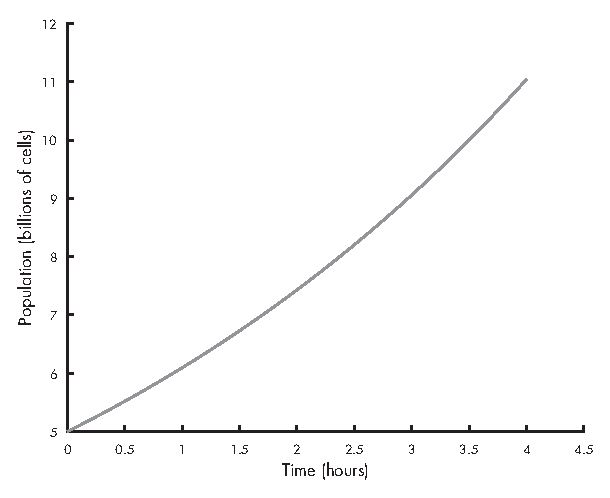
\includegraphics{book/images/figure09_01_new.eps}
\caption{Solution to a simple differential equation by Euler's method}
\label{fig:euler}
\end{figure}

As you can see, the population doubles in a little less than 4 hours.


\section{Solving ODEs with ode45}
\label{ode45}

A limitation of Euler's method is that it assumes that the derivative is constant between time steps, and that's not generally true.  Fortunately, there are better methods that estimate the derivative between time steps, and \linebreak they are much more accurate.

\index{time step} 
\index{ode45@\lstinline{ode45}}

MATLAB provides a function called \lstinline{ode45} that implements one of these methods.  In this section I'll explain how to use it; you can read more about how it works in ``\nameref{howode45}'' on page~\pageref{howode45}.

\index{rate function}
\index{function!rate}

In order to use \lstinline{ode45}, you have to write a function that evaluates $dy/dt$ as a function of $t$ and $y$.  Fortunately, we already have one, called \lstinline{rate_func}:

\begin{code}
function res = rate_func(t, y)
   a = 0.2;
   dydt = a * y;
   res = dydt;
end
\end{code}

We can call \lstinline{ode45} from the Command Window like this:

\begin{code}
***[T, Y] = ode45(@rate_func, [0, 4], 5);***
***plot(T, Y)***
\end{code}

The first argument is a function handle, as we saw in Chapter~\ref{fzero}.  The second argument is the time interval where we want to evaluate the solution; in this case the interval is from $t=0$ to $t=4$ hours.  The third argument is the initial population, 5 billion cells.

\index{function handle}
\index{handle!function}
\index{output variable}
\index{variable!output}

The \lstinline{ode45} function is the first function we've seen that returns \emph{two} output variables.
In order to store them, we have to assign them to two variables, \lstinline{T} and \lstinline{Y}. Figure~\ref{fig:runge} shows the results.

\begin{figure}[ht]
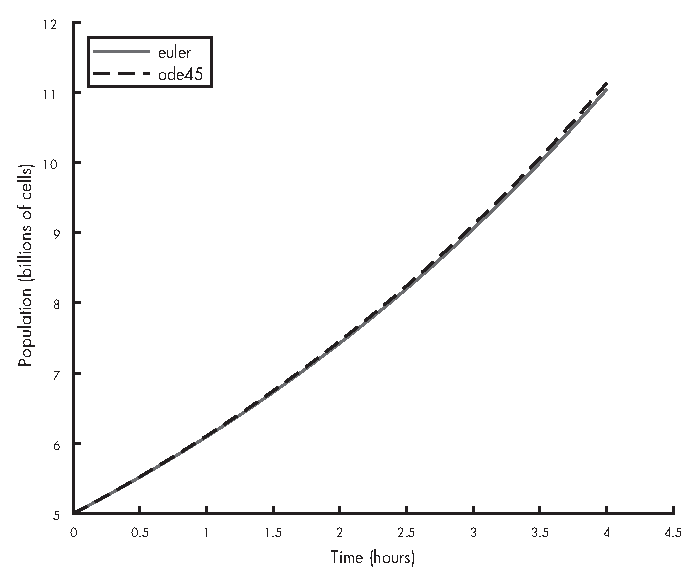
\includegraphics{book/images/figure09_02_new.eps}
\caption{Solutions to a simple differential equation using Euler's method and \lstinline{ode45}}
\label{fig:runge}
\end{figure}

The solid line is the estimate we computed with Euler's method; the dashed line is the solution from \lstinline{ode45}.

For the first 2--3 hours, the two solutions are visually indistinguishable.  During the last hour, they diverge slightly; at 4 hours, the difference is less than 1 percent.

For many purposes, the difference between Euler's method and \lstinline{ode45} is the least of our worries.  In this example, we probably don't know the initial population with perfect accuracy or the growth constant, \lstinline{a}.  Also, the assumption that the growth rate only depends on population is probably not true.  Any of these modeling errors could be bigger than 1 percent.

However, for some problems, Euler's method can be off by a lot more than 1 percent.  
In those cases \lstinline{ode45} is almost always more accurate, for two reasons: first, it computes the rate function several times per time step; second, if the time step is too big, \lstinline{ode45} can detect the problem and shrink the time step.  For more details, see ``\nameref{howode45}'' on page~\pageref{howode45}.


\section{Time Dependence}

Looking at \lstinline{rate_func} in the previous section, you might notice that it takes \lstinline{t} as an input variable but doesn't use it.  That's because the growth rate does not depend on time---bacteria don't know what time it is.

\index{time dependence}

But rats do.  Or, at least, they know what season it is.
Suppose that the growth rate for rats depends on the current population \emph{and} the availability of food, which varies over the course of the year.
The differential equation might be something like
%
\begin{equation*}
\frac{dy}{dt}(t) = a y(t) \left(1 - \cos (\omega t) \right)
\end{equation*}
%
where $t$ is time in days and $y(t)$ is the population at time $t$.
Because the growth rate depends on time, this differential equation is \emph{time dependent}.

The variables $a$ and $\omega$ are \emph{parameters}, which are values that
quantify a physical aspect of the scenario.  Parameters are often constants, but in some models they vary in time.

\index{parameter}

In this example, $a$ characterizes the reproductive rate per day, and
$\omega$ is the frequency of a periodic function that describes
the effect of varying food supply on reproduction.

We'll use the values $a = 0.002$
and $\omega = 2 \pi/365$ (one cycle per year).
The growth rate is lowest at $t=0$, on January~1, and highest at $t=365/2$, on June~30.

Now we can write a function that evaluates the growth rate:

\begin{code}
function res = rate_func(t, y)
    a = 0.002;
    omega = 2*pi / 365;
    res = a * y * (1 - cos(omega * t));
end
\end{code}

To test this function, I put it in a file called \emph{rats.m} with a top-level function called 
\lstinline{rats}:

\begin{code}
function res = rats()
    t = 365/2;
    y = 1000;
    res = rate_func(t, y);
end
\end{code}

The top-level function assumes, for purposes of testing, that
there are 1000 rats at $t=365/2$ (June~30) and computes the growth rate under those conditions.

We can run the top-level function like this:

\begin{code}
>> ***r = rats***

r = 4
\end{code}

Under these conditions, the growth rate is 4 new rats per day. 

Now that we've tested \lstinline{rate_func}, we can use \lstinline{ode45} to solve the differential equation.
Here's how to call it from the top-level function in \emph{rats.m}:

\begin{code}
[T, Y] = ode45(@rate_func, [0, 365], 1000)
plot(T, Y)
\end{code}

The first argument is a function handle, again.  The second argument is the interval we are interested in, a duration of one year, expressed in units of days.
The third argument is the initial population, $y(0) = 1000$.

\index{interval}

Figure~\ref{fig:rats} shows the results. 

\begin{figure}[ht]
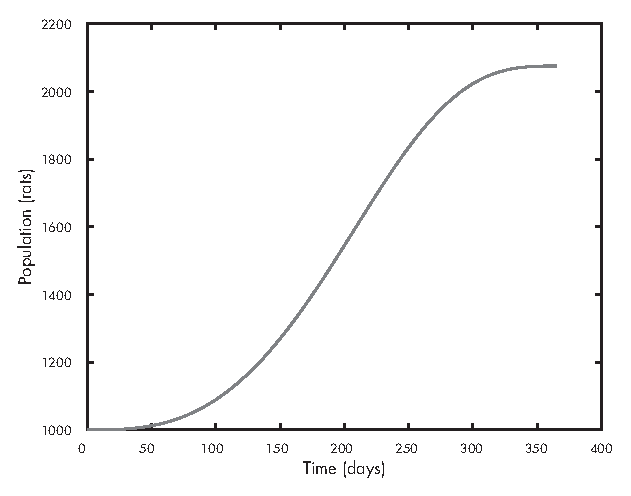
\includegraphics{book/images/figure09_03_new.eps}
\caption{Solutions to a simple differential equation by Euler's method and \lstinline{ode45}}
\label{fig:rats}
\end{figure}

The population grows slowly during the winter, quickly during the summer, and then slowly again in the fall.

To see the population at the end of the year, you can display the last element of \lstinline{Y}:

\begin{code}
Y(end)
2.0751e+03
\end{code}

That's a little more than 2000 rats, so the population roughly doubles in one year.

The index here is \lstinline{end}, which is a special word in MATLAB that means ``the index of the last element.''  You can use it in an expression, so \lstinline{Y(end - 1)} is the second-to-last element of
\lstinline{Y}.

\index{end statement@\lstinline{end} statement}
\index{index!end@\lstinline{end}}

\newpage
\section{What Could Go Wrong?}

Don't forget the \lstinline{@} on the function handle.
If you leave it out, like:

\begin{code}
[T, Y] = ode45(rate_func, [0, 365], 1000)
\end{code}
MATLAB treats the first argument as a function
call and calls \lstinline{rate_func} without providing arguments.
Then you get an error message:

\index{rate function}
\index{function handle}

\begin{code}
Not enough input arguments.

Error in rats>rate_func (line 18)
    res = a * y * (1 - cos(omega * t));

Error in rats (line 6)
    [T, Y] = ode45(rate_func, [0, 365], 1000);
\end{code}

Also, the rate function you write has to take two input variables, 
\lstinline{t} and \lstinline{y}, in that order, and return one output variable, 
\lstinline{res}.

\index{output variable}

If you're working with a rate function like:

\begin{equation*}
\frac{dy}{dt}(t) = a y(t)
\end{equation*}
you might be tempted to write this:

\begin{code}
function res = rate_func(y)        % WRONG
    a = 0.002;
    res = a * y;
end
\end{code}

But that would be wrong.  So very wrong.  Why?  Because
when \lstinline{ode45} calls \lstinline{rate_func}, it provides two arguments.
If you only take one input variable, you'll get an error.  So
you have to write a function that takes \lstinline{t} as an input
variable, even if you don't use it:

\index{input variable}

\begin{code}
function res = rate_func(t, y)     % RIGHT
    a = 0.002;
    res = a * y;
end
\end{code}

Another common error is to write a function that doesn't make
an assignment to the output variable.  If you write something
like:

\begin{code}
function res = rate_func(t, y)
    a = 0.002;
    omega = 2*pi / 365;
    r = a * y * (1 - cos(omega * t));    % WRONG
end
\end{code}
\newpage and then call it from \lstinline{ode45}, you get

\begin{code}
Output argument "res" (and maybe others) not assigned during call
to "rate_func".
\end{code}

I hope these warnings save you some time debugging.

\section{Labeling Axes}

The plots in this chapter have labels on the axes, and one of them has a legend, but I didn't show you how to do that.  Let's do it now.

\index{labeling axes}
\index{axes}
\index{xlabel@\lstinline{xlabel}}
\index{ylabel@\lstinline{ylabel}}

The functions to label the axes are \lstinline{xlabel} and \lstinline{ylabel}:

\begin{code}
xlabel('Time (hours)')
ylabel('Population (billions of cells)')
\end{code}

The function to generate a legend is \lstinline{legend}:

\begin{code}
legend('euler', 'ode45')
\end{code}

\index{legend@\lstinline{legend}}

The arguments are the labels for the lines, in the order they were drawn.  Usually the legend is in the upper-right corner, but you can move it by providing an optional argument called \lstinline{Location}:

\begin{code}
legend('euler', 'ode45', 'Location', 'northwest')
\end{code}

Finally,  save the figures using \lstinline{saveas}:

\begin{code}
saveas(gcf, 'runge.eps', 'epsc')
\end{code}

The first argument is the figure we want to save; \lstinline{gcf} is a MATLAB command that stands for ``get current figure,'' which is the figure we just drew.  The second argument is the filename.  The extension specifies the format we want, which is Encapsulated PostScript (\emph{.eps}).  The third argument tells MATLAB what driver to use.  The details aren't important, but \lstinline{epsc} generates figures in color.

\index{figure}
\index{get current figure}
\index{gcf@\lstinline{gcf}}
\index{saveas@\lstinline{saveas}}

\section{Chapter Review}

This chapter introduced \emph{differential equations (DE)}, which are equations that describe the
derivatives of an unknown function.
In an \emph{ordinary differential equation (ODE)}, all derivatives are taken with
respect to the same variable, as opposed to a \emph{partial differential equation (PDE)}, which includes derivatives with respect to more than one variable.

A \emph{first-order DE} includes only first derivatives, and a \emph{linear DE} includes no products or powers of the function and its derivatives.
A differential equation is \emph{time dependent} if the rate function depends on time.

When we solve a differential equation numerically, the \emph{time step} is the interval in time between successive elements of the solution.
A \emph{parameter} is a value that appears in a model to quantify some
physical aspect of the scenario being modeled.

Until now we have only put one function in each M-file, but in this chapter we wrote a \emph{top-level function}, which is the first function in an M-file, and a \emph{helper function}, which is any function in an M-file that is not the top-level function.

In the next chapter, we'll solve \emph{systems} of ODEs, which are used to describe physical systems with multiple parts that interact.
But first, here's an exercise where you can apply what you've learned so far.


\section{Exercise}

Before you go on, you might want to work on the following exercise.

\subsection{Exercise 1}

\index{coffee}
\index{cooling}
\index{Newton's law of cooling}

Suppose that you're given an 8-ounce cup of coffee at \SI{90}{\celsius}.
You have learned from bitter experience that the hottest coffee you
can drink comfortably is \SI{60}{\celsius}.  

If the temperature of the coffee drops by \SI{0.7}{\celsius} during the first minute, how long will you have to wait to drink your coffee?

You can answer this question with Newton's Law of Cooling (see \linebreak \url{https://greenteapress.com/matlab/newton}):
%
\begin{equation*}
\frac{dy}{dt}(t) = -k (y(t) - e)
\end{equation*}
%
where $y(t)$ is the temperature of the coffee at time $t$,
$e$ is the temperature of the environment, and $k$ is a parameter
that characterizes the rate of heat transfer from the coffee to the environment.

Let's assume that $e$ is \SI{20}{\celsius} and constant; that is, the coffee does not warm up the room.

Let's also assume $k$ is constant.  In that case, we can estimate it based on the information we have.  If the temperature drops \SI{0.7}{\celsius} during the first minute, when the coffee is \SI{90}{\celsius}, we can write
%
\begin{equation*}
-0.7 = -k (90 - 20)
\end{equation*}
%

Solving this equation yields $k = 0.01$.

Here are some suggestions for getting started:

\begin{enumerate}

\item Create a file named \emph{coffee.m} and write a function
called \lstinline{coffee} that takes no input variables.  Put a simple statement like \lstinline{x = 5} in the body of the function and invoke \lstinline{coffee} from the Command \linebreak Window.

\item Add a helper function called \lstinline{rate_func} that takes \lstinline{t} and \lstinline{y} and computes $dy/dt$.  In this case, \lstinline{rate_func} does not actually depend on $t$; nevertheless, your function has to take $t$ as the first input variable in order to work with \lstinline{ode45}.

\item Test your function by adding a line like \lstinline{rate_func(0, 90)}
to \lstinline{coffee}, then call \lstinline{coffee} from the Command Window.
Confirm that the initial rate is \SI{-0.7}{\celsius \per \minute}.

\item Once you get \lstinline{rate_func} working, modify
\lstinline{coffee} to use \lstinline{ode45} to compute the temperature
of the coffee for 60 minutes.  Confirm that
the coffee cools quickly at first, then cools more slowly, and reaches
room temperature after about an hour.

\item Plot the results and estimate the time when the temperature reaches~\SI{60}{\celsius}.

\end{enumerate}







\chapter{Systems of ODEs}
\label{systems}

In the previous chapter we used Euler's method and {\tt ode45} to solve a single first-order differential equation.  In this chapter we'll move on to systems of ODEs and implement a model of a predator-prey system.  But first, we have to learn more about matrices.


\section{Matrices}

A \emph{matrix} is a two-dimensional version of a vector.  Like a vector,
it contains elements that are identified by indices.  The difference
is that the elements are arranged in rows and columns, so it takes
{\em two} indices to identify an element.

\subsection{Creating a Matrix}

\index{matrix}
\index{index}

A common way to create a matrix is the {\tt zeros} function,
which returns a matrix with the given size filled with zeros.
This example creates a matrix with two rows and three columns.

\begin{code}
>> ***M = zeros(2, 3)***

M =  0     0     0
     0     0     0
\end{code}

If you don't know the size of a matrix, you can use {\tt whos} to display it:

\begin{code}
>> ***whos M***
  Name      Size            Bytes  Class     Attributes
  M         2x3                48  double   
\end{code}

Or the {\tt size} function, which returns a vector:

\index{whos@{\tt whos}}
\index{size@{\tt size}}

\begin{code}
>> ***V = size(M)***

V = 2    3
\end{code}

The first element is the number of rows, the second is the number of
columns.

\index{row}
\index{column}
\index{element}

To read an element of a matrix, you specify the row and column numbers:

\begin{code}
>> ***M(1,2)***

ans = 0

>> ***M(2,3)***

ans = 0
\end{code}

When you're working with matrices, it takes some effort to remember
which index comes first, row or column.  I find it useful to repeat
``row, column'' to myself, like a mantra.  You might also find it
helpful to remember ``down, across,'' or the abbreviation RC as in "radio control" or RC Cola.

Another way to create a matrix is to enclose the elements in
brackets, with semi-colons between rows:

\begin{code}
>> ***D = [1,2,3 ; 4,5,6]***

D =  1     2     3
     4     5     6

>> ***size(D)***

ans = 2     3
\end{code}

\index{semi-colon}

\subsection{Row and Column Vectors}
\label{rowvector}

\index{row vectors}
\index{column vector}
\index{vector!row}
\index{vector!column}

Although it's useful to think in terms of numbers, vectors and matrices,
from MATLAB's point of view, everything is a matrix.  A number
is just a matrix that happens to have one row and one column:

\begin{code}
>> ***x = 5;***
>> ***size(x)***

ans = 1     1
\end{code}

And a vector is a matrix with only one row:

\begin{code}
>> ***R = 1:5;***
>> ***size(R)***

ans = 1     5
\end{code}

Well, some vectors, anyway.  Actually, there are two kind
of vectors.  The ones we've seen so far are called {\em row vectors},
because the elements are arranged in a row; the other kind are
{\em column vectors}, where the elements are in a single column.

One way to create a column vector is to create a matrix with only
one element per row:

\begin{code}
>> ***C = [1;2;3]***

C =

     1
     2
     3

>> ***size(C)***

ans = 3     1
\end{code}

The difference between row and column vectors is important in
linear algebra, but for most basic vector operations, it doesn't matter.  
For example, when you index the elements of a vector, you don't have to know what kind
it is:

\index{linear algebra}

\begin{code}
>> ***R(2)***

ans = 2

>> ***C(2)***

ans = 2
\end{code}


\subsection{The Transpose Operator}
\index{Matrices!transpose}

The transpose operator, which looks remarkably like an apostrophe,
computes the {\em transpose} of a matrix, which is a new matrix
that has all of the elements of the original, but with each row
transformed into a column (or you can think of it the other way around).

\index{transpose operator}

In this example:

\begin{code}
>> ***D = [1,2,3 ; 4,5,6]***

D =  1     2     3
     4     5     6
\end{code}

{\tt D} has two rows, so its transpose has two columns:

\begin{code}
>> ***Dt = D'***

Dt = 1     4
     2     5
     3     6
\end{code}

\begin{ex}
What effect does the transpose operator
have on row vectors, column vectors, and numbers?
\end{ex}

\section{Solving Systems of ODEs}

Now that we've seen the basics of matrices, let's see how we can use them to solve systems of differential equations.

\subsection{Lotka-Volterra}
\label{lotka}

The Lotka-Volterra model describes the interactions between two
species in an ecosystem, a predator and its prey.  As an example, we'll consider foxes and rabbits.

\index{Lotka-Volterra model}
\index{rabbit}
\index{fox}
\index{system of ODEs}

The model is governed by the following system of differential equations:

\begin{eqnarray}
    \frac{dx}{dt} &=& a x - b x y         \\
    \frac{dy}{dt} &=& -c y + d x y       \\
\end{eqnarray}
%
where $x$ and $y$ are the populations of rabbits and foxes,
and $a$, $b$, $c$, and $d$ are parameters
that quantify the interactions between the two species (See
\url{https://greenteapress.com/matlab/lotka}.)

At first glance you might think you could solve these equations by
calling {\tt ode45} once to solve for $x$ and
once to solve for $y$.  The problem is that each equation involves
both variables, which is what makes this a {\em system of equations}
and not just a list of unrelated equations.  To solve a system, you
have to solve the equations simultaneously.

\index{system of equations}
\index{ode45@{\tt ode45}}

Fortunately, {\tt ode45} can handle systems of equations.  The
difference is that the initial condition is a vector that contains
initial values $x(0)$ and $y(0)$, and the output is a matrix
that contains one column for $x$ and one for $y$.

\index{rate function}

Listing~\ref{lst:lotka_volterra} shows the rate function
with the parameters $a = 0.1$, $b = 0.01$, $c = 0.1$, and $d = 0.002$:

\begin{lstlisting}[caption={A rate function for Lotka-Volterra}, label={lst:lotka_volterra}]
function res = rate_func(t, V)
    % unpack the elements of V
    x = V(1);
    y = V(2);

    % set the parameters
    a = 0.1;
    b = 0.01;
    c = 0.1;
    d = 0.002;

    % compute the derivatives
    dxdt = a*x - b*x*y;
    dydt = -c*y + d*x*y;

    % pack the derivatives into a vector
    res = [dxdt; dydt];
end
\end{lstlisting}

The first input variable, {\tt t}, is time.
Even though the time variable is not used in this rate function,
it has to be there in order for this function to work with {\tt ode45}.

The second input variable, {\tt V}, is a vector with two elements,
$x(t)$ and $y(t)$.

The body of the function includes four sections, each explained by a comment.

The first section {\em unpacks} the vector by copying the elements
into variables.  This isn't necessary, but giving names to
these values helps me remember what's what.  It also makes the third
section, where we compute the derivatives, resemble the mathematical
equations we were given, which helps prevent errors.

\index{pack vector}
\index{unpack vector}

The second section sets the parameters that describe the
reproductive rates of rabbits and foxes, and the characteristics of
their interactions.  If we were studying a real system, these values
would come from observations of real animals, but for this example
I chose values that yield interesting results.

\index{parameter}

The third section computes the derivatives of $x$ and $y$ using the equations
we were given.

The last section {\em packs} the computed derivatives back into a
vector.  When {\tt ode45} calls this function, it provides a vector
as input and expects to get a vector as output.

Sharp-eyed readers will notice something different about this line:

\begin{code}
    res = [drdt; dfdt];
\end{code}

The semi-colon between the elements of the vector is not an error.  It
is necessary in this case because {\tt ode45} requires the result of
this function to be a column vector.

\index{semi-colon}

As always, it's a good idea to test your rate function before you call {\tt ode45}.  
I created a file named {\em lotka.m} with the following top-level function:

\begin{code}
function res = lotka()
    t = 0;
    V_init = [80, 20];
    rate_func(t, V_init)
end
\end{code}

\index{initial condition}

\verb"V_init" is a vector that represents the initial condition, 80 rabbits and 20 foxes.  
The result from \verb"rate_func" is:

\begin{code}
-8.0000
 1.2000
 \end{code}
  
Which means that with these initial conditions, we expect the rabbit population to decline initially at a rate of 8 per week, and the fox population to increase by 1.2 per week.  
  
Now we can run {\tt ode45} like this:

\begin{code}
tspan = [0, 200]
[T, M] = ode45(@rate_func, tspan, V_init)
\end{code}

The first argument is the function handle for the rate function.
The second argument is the time span, from 0 to 200 weeks.
The third argument is the initial condition.

\index{function handle}
\index{handle!function}


\subsection{Output Matrices}

{\tt ode45} returns two values: {\tt T}, which is a vector, 
and {\tt M}, which is a matrix.

\begin{code}
>> ***size(T)***
ans = 101     1

>> ***size(M)***
ans = 101     2
\end{code}

{\tt T} has 101 rows and one column, so it is a column vector with one row for
each time step.

{\tt M} has 101 rows, one for each time step, and 2 columns, one for each variable,
$x$ and $y$.

This structure -- one column per variable -- is a common way to
use matrices.  {\tt plot} understands this structure, so if you
do this:

\begin{code}
>> ***plot(T, M)***
\end{code}

MATLAB understands that it should plot each column from {\tt M}
versus {\tt T}.

\index{colon}

You can copy the columns of {\tt M} into other variables like
this:

\begin{code}
>> ***R = M(:, 1)***;
>> ***F = M(:, 2);***
\end{code}

In this context, the colon represents the range from 1 to {\tt end},
so {\tt M(:, 1)} means ``all the rows, column 1'' and
{\tt M(:, 2)} means ``all the rows, column 2.''

\begin{code}
>> ***size(R)***
ans = 101     1

>> ***size(F)***
ans = 101     1
\end{code}

So {\tt R} and {\tt F} are column vectors.

\index{column vector}

Now we can plot these vectors separately, which makes it easier to give them different style strings:

\begin{code}
>> ***plot(T, R, '-')***
>> ***plot(T, F, '--')***
\end{code}

\begin{figure}[ht]
\centerline{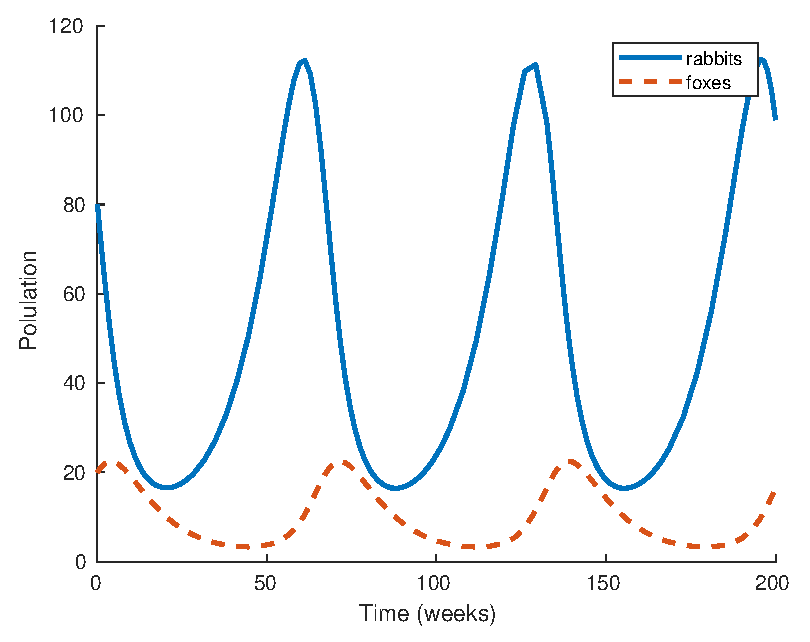
\includegraphics[height=3in]{book/figs/lotka.eps}}
\caption{Solution for the Lotka-Volterra model.}
\label{fig:lotka}
\end{figure}

Figure~\ref{fig:lotka} shows the results. The x-axis is time in weeks; the y-axis is population.  The top curve shows the population of rabbits; the bottom curve shows foxes.

\index{boom and bust}

Initially there are too many foxes, so the rabbit population declines.  Then there are not enough rabbits, and the fox population declines.  That allows the rabbit population to recover, and the pattern repeats.

This cycle of ``boom and bust'' is typical of the Lotka-Volterra model.


\subsection{Phase Plot}

Instead of plotting the two populations over time, it is sometimes useful to plot them against each other:

\begin{code}
>> ***plot(R, F)***
\end{code}
\begin{figure}[ht]

\centerline{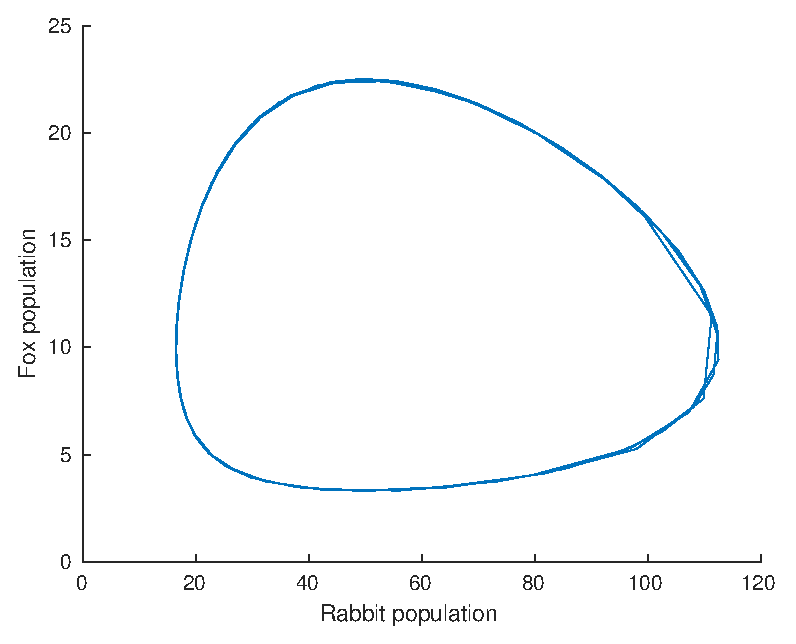
\includegraphics[height=3in]{book/figs/phase.eps}}
\caption{Phase plot from the Lotka-Volterra model.}
\label{fig:phase}
\end{figure}

Figure~\ref{fig:phase} shows the result.  
Each point on this plot represents a certain number of rabbits (on the
x axis) and a certain number of foxes (on the y axis).
Since these are the only two variables in the system, each point in
this plane describes the complete state of the system, that is, the values of
the variables we're solving for.

\index{phase plot}
\index{trajectory}
\index{state}

Over time, the state moves around the plane; Figure~\ref{fig:phase} shows
the path traced by the state over time; this path
is called a {\em trajectory}.

Since the behavior of this system is periodic, the trajectory is a loop.

If there are 3 variables in the system, we need 3 dimensions to show
the state of the system, so the trajectory is a 3-D curve.
You can use {\tt plot3} to trace trajectories in 3 dimensions,
but for 4 or more variables, you're on your own.

\index{plot3@{\tt plot3}}


\subsection{What Could Go Wrong?}

The output vector from the rate function has to be a column vector; otherwise you get an error:

\begin{code}
Error using odearguments (line 93)
RATE_FUNC must return a column vector.
\end{code}

Which is a pretty good error message.  It's not clear {\em why}
it needs to be a column vector, but that's not our problem.

\index{column vector}

Another possible error is reversing the order of the elements in the
initial conditions, or the vectors inside {\tt lotka}.  MATLAB
doesn't know what the elements are supposed to mean, so it can't catch
errors like this; it will just produce incorrect results.

The order of the elements (rabbits and foxes) is up to you, but
you have to be consistent.  That is, the order of the initial conditions you
provide when you call {\tt ode45} has to be the same as the order,
inside \verb"rate_func", where you unpack the input vector, and the
same as the order of the derivatives in the output vector.

\section{Summary}

In this chapter, we use {\tt ode45} to solve a system of first order differential equations.
As an exercise, you'll have a chance to solve the famous Lorenz equations, one of the first
examples of a chaotic system.

In the next chapter, we move on to second-order systems, which we will use to describe systems
with objects moving in space, governed by Newton's laws of motion.


\section{Glossary}

\begin{description}

\item[row vector:] A matrix that has only one row.

\item[column vector:] A matrix that has only one column.

\item[transpose:] An operation that transforms the rows of a matrix
into columns (or the other way around, if you prefer).

\item[system of equations:] A collection of equations written in terms of
the same set of variables.

\item[unpack:] To copy the elements of a vector into a set of variables.

\item[pack:] To copy values from a set of variables into a vector.

\item[state:] If a system can be described by a set of variables,
the values of those variables are called the state of the system.

\item[phase plot:] A plot that shows the state of a system as point
in the space of possible states.

\item[trajectory:] A path in a phase plot that shows how the state of
a system changes over time.


\end{description}

\section{Exercises}

\begin{ex}

\index{Lorenz attractor}

Based on the examples we've seen so far, you'd think that all ODEs describe population as
a function of time, but that's not true.

According to Wikipedia, ``The Lorenz attractor, introduced by Edward Lorenz in 1963, is a
non-linear three-dimensional deterministic dynamical system derived
from the simplified equations of convection rolls arising in the
dynamical equations of the atmosphere. For a certain set of parameters
the system exhibits chaotic behavior and displays what is today called
a strange attractor...'' (see \url{https://greenteapress.com/matlab/lorenz}).

The system is described by this system of differential equations:
%
\begin{eqnarray}
x_t &=& \sigma (y - x)  \\
y_t &=& x (r - z) - y   \\
z_t &=& xy - b z
\end{eqnarray}
%
Common values for the parameters are $\sigma = 10$, $b = 8/3$, and $r=28$.

Use {\tt ode45} to estimate a solution to this system of equations.


\begin{enumerate}

\item Create a file named {\em lorentz.m} with a top-level function named {\tt lorenz} and a helper function named \verb"rate_func".

\item  The rate function should
takes {\tt t} and {\tt V} as input variables, where the components
of {\tt V} are understood to be the current values of {\tt x},
{\tt y} and {\tt z}.  It should compute the corresponding derivatives
and return them in a single column vector.

\item Test the function by calling it from the top-level function with values like $t=0$, $x=1$, $y=2$, and $z=3$.  
Once you get your function working, you should make it a silent function before calling {\tt ode45}.

\item Use {\tt ode45} to estimate the solution for the time span $[0, 30]$
with the initial condition $x=1$, $y=2$, and $z=3$.

\item Plot the results as a time series, that is, each of the variables as a function of time.

\item Use {\tt plot3} to plot the trajectory of $x$, $y$, and $z$.

\end{enumerate}

% lorenz.m
\end{ex}



\chapter{Second-Order Systems}


So far we've seen first-order differential equations and systems of first-order ODEs.  In this chapter, we'll introduce second-order systems, which are particularly useful for modeling Newtonian motion.

\index{Newtonian motion}
\index{Newton's law of motion}

\section{Newtonian Motion}

Newton's second law of motion is often written like this:

\begin{equation*}
    F = m a
\end{equation*}
where $F$ is the net force acting on an object, $m$ is the
mass of the object, and $a$ is the acceleration of the object.

This equation suggests
that if you know $m$ and $a$, you can compute the force. And that's true,
but in most physical simulations it's the other way around: based on a
physical model, you know $F$ and $m$, and you compute $a$.

\index{second derivative}
\index{second-order differential equation}
\index{differential equation!second-order}

So if we know acceleration as a function of time, how do we
find the position of the object, $r$?  Well, we know that acceleration
is the second derivative of position, so we can write the differential
equation

\begin{equation*}
    \frac{d^2r}{dt^2} = a
\end{equation*}
where ${d^2r}/{dt^2}$ is the second time derivative of $r$.

Because this equation includes a second derivative, it's
a second-order ODE.  We can't solve the equation using \lstinline{ode45} in this form, but
by introducing a new variable, \emph{v}, for velocity, we can rewrite it
as a system of first-order ODEs:

\begin{eqnarray*}
    \frac{dr}{dt} &=& v   \\
    \frac{dv}{dt} &=& a
\end{eqnarray*}

The first equation says that the first derivative of $r$ is $v$;
the second equation says that the first derivative of $v$ is $a$.


\section{Free Fall}
\label{freefall}

As an example of Newtonian motion, let's go back to the question from Section~\ref{penny}:

\begin{quote}
If you drop a penny from the top of the Empire State Building, how long does it take to reach the sidewalk, and how fast is it going when it gets there?
\end{quote}

We'll start with no air resistance; then we'll add air resistance to the model and see what effect it has.

\index{air resistance}
\index{gravity}

Near the surface of the earth,
acceleration due to gravity is \SI{-9.8}{\meter \per \second \squared}, where the minus sign
indicates that gravity pulls down.
If the object falls straight down, we can describe its position with a
scalar value $y$, representing altitude.

\index{position}
\index{velocity}
\index{rate function}
Listing~\ref{lst:penny_rate_func} contains a rate function we can use with \lstinline{ode45} to solve
this problem:

\begin{lstlisting}[caption={A rate function for the falling penny problem}, label={lst:penny_rate_func}]
function res = rate_func(t, X)
    % unpack position and velocity
    y = X(1);      
    v = X(2);      
    
    % compute the derivatives
    dydt = v;
    dvdt = -9.8;

    % pack the derivatives into a column vector
    res = [dydt; dvdt];
end
\end{lstlisting}

The rate function in Listing~\ref{lst:penny_rate_func} takes \lstinline{t} and \lstinline{X} as input variables, where the elements of \lstinline{X} are understood to be the position and velocity of the penny.

It returns a column vector that contains \lstinline{dydt} and \lstinline{dvdt}, which
are velocity and acceleration, respectively.
Since velocity is the second element of \lstinline{X}, we can simply assign this value to \lstinline{dydt}.
And since the derivative of velocity is acceleration, we can assign the acceleration due to gravity to \lstinline{dvdt}.

\index{column vector}
\index{acceleration}

As always, we should test the rate function before we call \lstinline{ode45}.  Here's the top-level function we can use to test it:

\begin{code}
function penny()
   t = 0;
   X = [381, 0];
   rate_func(t, X)
end
\end{code}

The initial condition of \lstinline{X} is the initial position, which is the height of the Empire State Building, about \SI{381}{\meter}, and the initial velocity, which is \SI{0}{\meter \per \second}.

\index{Empire State Building}
\index{penny}

The result from \lstinline{rate_func} is

\begin{code}
    0
   -9.8000
\end{code}
which is what we expect.

Now we can run \lstinline{ode45} with this rate function:

\begin{code}
tspan = [0, 10]
[T, M] = ode45(@rate_func, tspan, X)
\end{code}

As always, the first argument is the function handle, the second
is the time span (10 seconds), and the third is the initial
condition.

The result is a vector, \lstinline{T}, that contains the time values, and a matrix, \lstinline{M}, that contains two columns, one for altitude and one for velocity.
\index{function handle}
\index{time span}
\index{matrix}

We can extract the first column and plot it, like this:

\begin{code}
Y = M(:, 1)
plot(T, Y)
\end{code}


\begin{figure}
\centerline{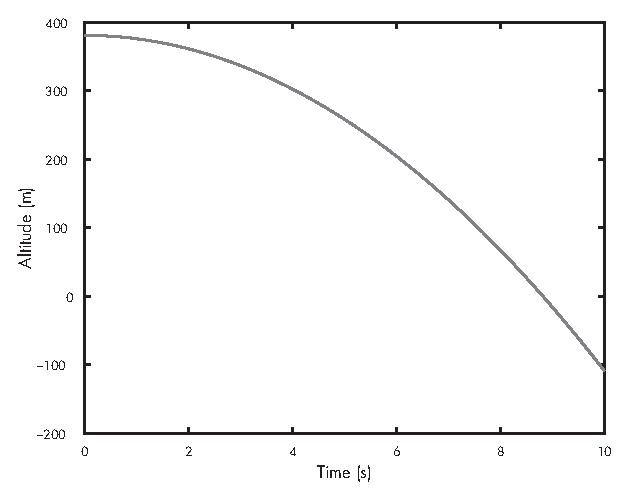
\includegraphics[scale=0.8]{images/figure11_01_new.eps}}
\caption{Altitude versus time for an object in free fall}
\label{fig:penny}
\end{figure}

Figure~\ref{fig:penny} shows the result.  Altitude drops slowly at first and picks up speed.  Between 8 and 9 seconds, the altitude reaches 0, which means the penny hits the sidewalk.  But \lstinline{ode45} doesn't know where the ground is, so  the penny keeps going through 0 into negative altitude.  We'll solve that problem in the next section.

\section{ODE Events}
\label{events}

\index{ODE event}

Normally when you call \lstinline{ode45} you specify a start time and
an end time.  But sometimes you don't know ahead of time when the
simulation should end.  To solve this problem we can define an \emph{event}, 
something of interest that happens during a simulation,
like the penny reaching the ground.

Here are the steps: 

\index{event function}
\index{function!event}
\index{ODE event}

\begin{enumerate}

\item First we define an \emph{event function} that allows \lstinline{ode45} to figure out when
an event occurs.  Here's an event function for the penny example:

\begin{code}
function [value, isterminal, direction] = event_func(t,X)
    value = X(1);
    isterminal = 1;
    direction = -1;
end
\end{code}

The event function takes the same input variables as the rate function and returns three output variables: \lstinline{value} determines when an event can occur, \lstinline{direction} determines whether it does, and \lstinline{isterminal} determines what happens.
More specifically, an event can occur when \lstinline{value} passes through 0.
If \lstinline{direction} is positive, the event only occurs if \lstinline{value} is increasing.
 If \lstinline{direction} is negative, the event only occurs if \lstinline{value} is decreasing.
If \lstinline{direction} is 0, the event always occurs.
If \lstinline{isterminal} is 1, the event causes the simulation to end; if it is 0, the simulation continues.

This event function uses the altitude of the penny as \lstinline{value} so an event can occur when altitude passes through 0.  
Because \lstinline{direction} is negative, an event occurs only when altitude is decreasing, and
because \lstinline{isterminal} is 1, the simulation ends if an event occurs.

\index{odeset@\lstinline{odeset}}
\index{options@\lstinline{options}}

\item Next, we use \lstinline{odeset} to create an object called \lstinline{options}:

\begin{code}
options = odeset('Events', @event_func);
\end{code}
%
The name of the option is \lstinline{Events} and the value is the handle of the event function.  

\item Finally, we pass \lstinline{options} as a fourth argument to \lstinline{ode45}:

\begin{code}
[T, M] = ode45(@rate_func, tspan, X, options);
\end{code}

When \lstinline{ode45} runs, it invokes \lstinline{event_func} after each time step.  If the event function indicates that a terminal event occurred, 
\lstinline{ode45} stops the simulation.

\end{enumerate}

Let's look at the results from the penny example:  

\begin{code}
>> T(end)
8.8179

>> M(end, :)
0.0000  -86.4153
\end{code}

The last value of \lstinline{T} is about 8.8, which is the number of seconds the penny takes to reach the sidewalk.

The last row of \lstinline{M} indicates that the final altitude is 0, which is what we wanted, and the final velocity is about \SI{-86}{\meter \per \second}.


\section{Air Resistance}
\label{air_resistance}

\index{drag}
\index{air resistance}

To make this simulation more realistic, we can add air resistance.
For large objects moving quickly through air, the force due to air resistance, called \emph{drag}, is proportional to velocity squared.  
For an object falling down, drag is
directed up, so if velocity is negative, drag force is positive.

% b is used in the book "Physics for Scientists and Engineers" by Paul A. Tipler.
%TODO: consider writing out the drag equation

Here's how we can compute the force of drag as a function of velocity in one dimension:

\begin{equation*}
    f_\mathrm{d} = -\mathrm{sign}(v) b v^2 
\end{equation*}
where $v$ is velocity and
$b$ is a drag constant that depends on the density of
air, the cross-sectional area of the object, and the shape
of the object.  

The sign or signum function returns the value $1$ for positive values of 
$v$ and $-1$ for negative values.  So $f_\mathrm{d}$ is always in the opposite direction of $v$.

\index{signum function}
\index{sign@\lstinline{sign}}
\index{mass}
\index{terminal velocity}

To convert from force to acceleration we have to know mass, but that's easy to find: the mass of a penny is about \SI{2.5}{\gram}.  It's not as easy to find the drag constant, but based on reports that the terminal velocity of a penny is about \SI{18}{\meter \per \second}, I've estimated that it's about \SI{75e-6}{\kilogram \per \meter}.

Listing~\ref{lst:acceleration_drag} defines a function that takes \lstinline{t} and \lstinline{X} as input variables and returns the total acceleration of the penny due to gravity and drag:

\begin{lstlisting}[caption={Calculating acceleration of a penny with drag}, label={lst:acceleration_drag}]
function res = acceleration(t, X)
    b = 75e-6;                 % drag constant in kg/m
    v = X(2);                  % velocity in m/s
    f_d = -sign(v) * b * v^2;  % drag force in N

    m = 2.5e-3;               % mass in kg
    a_d = f_d / m;            % drag acceleration in m/s^2

    a_g = -9.8;               % acceleration of gravity in m/s^2
    res = a_g + a_d;          % total acceleration
end
\end{lstlisting}

First, we compute force due to drag .
Then we compute acceleration due to drag .
Lastly, we compute total acceleration due to drag and \mbox{gravity}.

\index{acceleration}
\index{force}

Be careful when you're working with forces and accelerations; make sure
you only add forces to forces or accelerations to accelerations.  In my
code, I use comments to remind myself what units the values have.
That helps me avoid errors like adding forces to accelerations.

To use this function, we make a small change in \lstinline{rate_func}:

\begin{code}
function res = rate_func(t, X)
    y = X(1);      
    v = X(2);      
    
    dydt = v;
    dvdt = acceleration(t, X);   % this line has changed

    res = [dydt; dvdt];
end

\end{code}

In the previous version, \lstinline{dvdt} is always \lstinline{-9.8}, the acceleration due to gravity.
In this version, we call \lstinline{acceleration} to compute the total acceleration due to gravity and drag .

\begin{figure}[ht]
\centerline{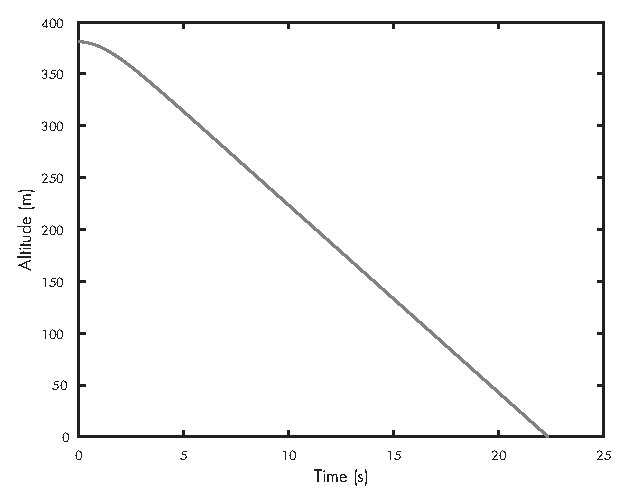
\includegraphics[scale=0.8]{images/figure11_02_new.eps}}
\caption{Altitude versus time for a penny in free fall with air resistance}
\label{fig:penny2}
\end{figure}

Everything else is the same.  Figure~\ref{fig:penny2} shows the result. 

Air resistance makes a big difference! Velocity increases until
acceleration due to drag equals acceleration due to gravity; after that, velocity is constant and position decreases linearly (and much more slowly than it would in a vacuum).

With air resistance, the time until the penny hits the sidewalk is \SI{22.4}{\second}, substantially longer than before (\SI{8.8}{\second}).

And the final velocity is \SI{18.1}{\meter \per \second}, substantially slower than before (\SI{86}{\meter \per \second}).

\section{Chapter Review}

In this chapter, we used Newton's laws of motion to write a differential equation that describes the motion of a falling penny.  

We rewrote that equation as a system of first-order differential equations so we could use \lstinline{ode45} to solve it.  Then we ran simulations of a falling penny with and without air resistance, also known as \emph{drag}.

We defined an \emph{event} as something of interest that happens during a simulation, like a collision between moving objects, and we wrote an \emph{event function}, which allows \lstinline{ode45} to figure out when an event occurs.

In the next chapter, we extend Newtonian motion to two dimensions and model the flight of a baseball.


\section{Exercises}

Before you go on, you might want to work on the following exercises.

\subsection{Exercise 1}
\index{skydiver}
\index{parachute}

In this exercise we'll model the descent of a skydiver, taking into account the change in drag when the parachute opens.

\begin{enumerate}

\item Modify the penny code from this chapter to simulate the descent of a \SI{75}{\kilogram} skydiver from an initial altitude of \SI{4000}{\meter}.
The drag constant for a skydiver without a parachute is about \SI{0.2}{\kilogram \per \meter}.
What would the velocity of the skydiver be on impact?
 
\item After opening their parachute, the velocity of the skydiver slows to about \SI{5}{\meter\per\second}.  Use your simulation to find the drag constant that yields a terminal velocity of \SI{5}{\meter\per\second}.

\item Increase the mass of the skydiver, and confirm that terminal velocity increases.  This phenomenon is the source of the intuition that heavy objects fall faster; in air, they do!

\item Now suppose the skydiver free falls until they get to an altitude of \SI{1000}{\meter} before opening the parachute.  How long would it take them to reach the ground?

\item What is the lowest altitude where the skydiver can open the parachute and still land at less than \SI{6}{\meter\per\second} (assuming that the parachute opens and deploys instantly)?

\end{enumerate}

% skydiver.m




\subsection{Exercise 2}
\label{earth}

\index{Earth}
\index{Sun}
\index{Law of Universal Gravitation}

Here's a question from the website \emph{Ask an Astronomer} (see \url{https://greenteapress.com/matlab/astro}):

\begin{quote}
If the Earth suddenly stopped orbiting the Sun, I know eventually it would be pulled in by the Sun's gravity and hit it. How long would it take the Earth to hit the Sun? I imagine it would go slowly at first and then pick up speed.
\end{quote}

Use \lstinline{ode45} to answer this question.  Here are some suggestions about how to proceed:

\begin{enumerate}

\item Look up the Law of Universal Gravitation and any constants you need. I suggest you work entirely in SI units: meters, kilograms, and newtons.

\item When the distance between the Earth and the Sun gets small, this system behaves badly, so you should use an event function to stop when the surface of the Earth reaches the surface of the Sun.

\item Express your answer in days, and plot the results as millions of kilometers versus days.

\end{enumerate}

% earth.m



% chpt11



\chapter{Two Dimensions}

In the previous chapter, we solved a one-dimensional problem, a penny falling from the Empire State Building.  Now we'll solve a two-dimensional problem, finding the trajectory of a baseball.

\index{baseball}

To do that, we'll use spatial vectors to represent quantities in two and three dimensions, including force, acceleration, velocity, and position.

\section{Spatial Vectors}
\label{spacial}

The word ''vector'' means different
things to different people.  In MATLAB, a vector is a matrix that has
either one row or one column.  So far we've used MATLAB vectors to
represent:

\begin{description}

\item[sequences:] A mathematical sequence, like the Fibonacci numbers, is a set of values identified by integer indices; in Chapter~\ref{vecseq}, we used a MATLAB vector to store the elements of a sequence. 

\item[state vectors:] A state vector is a set of values that
describes the state of a physical system.  When you call
{\tt ode45}, you give it initial conditions in a state
vector.  Then when {\tt ode45} calls your rate function, it
gives you a state vector.

\item[time series:] One of the results from {\tt ode45} is a vector that represents a sequence of time values.

\end{description}

\index{vector!spatial}
\index{spatial vector}
\index{sequence}
\index{state}
\index{time series}

In this chapter we'll see another use of MATLAB vectors: representing
\emph{spatial vectors}.  A spatial vector represents a multidimensional physical quantity like position, velocity, acceleration, or force.

\index{position}

For example, to represent a position in two-dimensional space, we can use a vector with two elements:

\begin{code}
>> P = [3 4]
\end{code}

To interpret this vector, we have to know what coordinate system it is defined in.  Most commonly, we use a Cartesian system where the x-axis points east and the y-axis points north.  In that case {\tt P} represents a point 3 units east and 4 units north of the origin.

\index{Cartesian system}
\index{magnitude}
\index{direction}
\index{Pythagorean theorem}

When a spatial vector is represented in this way, we can use it to compute the magnitude and direction of a physical quantity.  
For example, the {\em magnitude} of {\tt P} is the distance from the origin to {\tt P}, which is the hypotenuse of the triangle with sides {\tt P(1)} and {\tt P(2)}.  
We can compute it using the Pythagorean theorem:

\begin{code}
>> sqrt(P(1)^2 + P(2)^2)
ans = 5
\end{code}

Or we can do the same thing using the function {\tt norm}, which computes the
``Euclidean norm'' of a vector, which is its magnitude:

\index{norm@{\tt norm}}
\index{Euclidean norm}

\begin{code}
>> norm(P)
ans = 5
\end{code}

There are two ways to get the direction of a vector.  One convention is to compute the angle between the vector and the x-axis:

\begin{code}
>> atan2(P(2), P(1))
ans = 0.9273
\end{code}

In this example, the angle is about \SI{0.9}{\radian}.  But for computational purposes, we often represent direction with a \emph{unit vector}, which is a vector with length 1.  To get a unit vector we can divide a vector by its length:

\begin{code}
function res = hat(V)
    res = V / norm(V)
end
\end{code}
 
This function takes a vector, {\tt V}, and returns a unit vector with the same direction as {\tt V}.  It's called {\tt hat} because in mathematical notation, unit vectors are written with a ``hat'' symbol.  
For example, the unit vector with the same direction as $\vec{P}$ would be written $\uvec{P}$. 

\index{unit vector}
\index{vector!unit}

\section{Adding Vectors}

Vectors are useful for representing quantities like force and acceleration because we can add them up without having to think explicitly about direction.

\index{force}
\index{acceleration}

As an example, suppose we have two vectors representing forces:

\begin{code}
>> A = [2, 4];
>> B = [2, -2];
\end{code}

{\tt A} represents a force pulling northeast; {\tt B} represents a force pulling southeast, as shown in Figure~\ref{fig:vector2}

\begin{figure}[ht]
\centerline{\includegraphics[height=3in]{book/figs/vector2.eps}}
\caption{The sum of two forces represented by vectors.}
\label{fig:vector2}
\end{figure}

To compute the sum of these forces, all we have to do is add the vectors:

\begin{code}
>> A + B
ans = 4     2
\end{code}

Later in the chapter, we'll use vector addition to add accelerations due to different forces acting on a baseball.


\section{ODEs in Two Dimensions}
\label{projectile}

So far we've used {\tt ode45} to solve a system of first-order equations and a single second-order equation.  Now we'll take one more step, solving a system of second-order equations.

As an example, we'll simulate the flight of a baseball.
If there is no wind and no spin on the ball, the ball travels in a vertical plane, so we can think of the system as two-dimensional, with $x$ representing the horizontal distance
travelled from the starting place and $y$ representing height or altitude.

\index{baseball}
\index{altitude}
\index{rate function}

Listing~\ref{lst:baseball_rate_func} shows a rate function we can use to simulate this system with {\tt ode45}:

\begin{lstlisting}[caption={A rate function we can use to model the flight of a baseball}, label={lst:baseball_rate_func}]
function res = rate_func(t, W)
    P = W(1:2);
    V = W(3:4);

    dPdt = V;
    dVdt = acceleration(t, P, V);

    res = [dPdt; dVdt];
end

function res = acceleration(t, P, V)
    g = 9.8;             % acceleration of gravity in m/s^2
    a_gravity = [0; -g];
    res = a_gravity;
end
\end{lstlisting}

The second argument of \verb"rate_func" is understood to be a vector,
{\tt W}, with four elements.  The first two are assigned to {\tt P},
which represents position; the last two are assigned to {\tt V}, which
represents velocity. Both {\tt P} and {\tt V} have two elements
representing the $x$ and $y$ components.

\index{derivative}
\index{velocity}

The goal of the rate function is to compute the derivative of {\tt W}, so the output has to be a vector with four elements, where the first two represent the derivative of {\tt P}  and the last two represent the derivative of {\tt V}.
The derivative of {\tt P} is velocity.  We don't have to compute it; we were given it as part of {\tt W}.
The derivative of {\tt V} is acceleration.  To compute it, we call {\tt acceleration}, which takes as input variables time, position, and velocity.  In this example, we don't use any of the input variables, but we will soon.

\index{air resistance}
\index{gravity}

For now we'll ignore air resistance, so the only force on the baseball is gravity.  We represent acceleration due to gravity with a vector that has magnitude {\tt g} and direction along the negative $y$ axis.

Let's assume that a ball is batted from an initial position \SI{1}{\meter} above home plate, with an initial velocity of \SI{40}{\meter\per\second} in the horizontal and \SI{30}{\meter\per\second} in the vertical direction.

\index{initial condition}

Here's how we can call {\tt ode45} with these initial conditions:
 
\begin{code}
    P = [0; 1];       % initial position in m
    V = [40; 30];     % initial velocity in m/s
    W = [P; V];       % initial condition
    
    tspan = [0 8]
    [T, M] = ode45(@rate_func, tspan, W);
\end{code}

{\tt P} and {\tt V} are column vectors because we put semi-colons between the elements.  
So {\tt W} is a column vector with four elements.
{\tt tspan} specifies that we want to run the simulation for \SI{8}{\second}.

\index{time span}
\index{output variable}

The output variables from {\tt ode45} are a vector, 
{\tt T}, that contains time values and a matrix, {\tt M}, with four columns: the first two are position; the last two are velocity.

Here's how we can plot position as a function of time:

\begin{code}
	X = M(:, 1);
    Y = M(:, 2);
    
    plot(T, X)
    plot(T, Y)
\end{code}

{\tt X} and {\tt Y} get the first and second columns from {\tt M}, which are the $x$ and $y$ coordinates of position.

\begin{figure}[ht]
\centerline{\includegraphics[height=3in]{book/figs/baseball1.eps}}
\caption{Simulated flight of a baseball neglecting drag force.}
\label{fig:baseball1}
\end{figure}

Figure~\ref{fig:baseball1} shows what these coordinates look like as a function of time.  The $x$ coordinate increases linearly because the $x$ velocity is constant.  The $y$ coordinate goes up and down, as we expect.

The simulation ends just before the ball lands, having traveled almost \SI{250}{\meter}.  That's substantially farther than a real baseball would travel, because we have ignored air resistance, or ``drag force''.


\section{Drag Force}
\label{drag}

\index{drag}
\index{force!drag}

A simple model for the drag force on a baseball is:

\begin{equation}
    \vec{F_d} = - \frac{1}{2} ~ \rho v^2 C_d A \uvec{V}
\end{equation}

where $\vec{F_d}$ is a vector that represents the force on the baseball
due to drag, 
$\rho$ is the density of air, 
$C_d$ is the drag coefficient, and
$A$ is the cross-sectional area .

\index{drag coefficient}
\index{coefficient!drag}

$\vec{V}$ is the baseball's velocity vector; $v$ is the magnitude of $V$ and $\uvec{V}$ is a unit vector in the same direction as $V$.  The minus sign at the beginning means that the result is in the opposite direction of $V$.

\index{unit vector}

The function in Listing~\ref{lst:baseball_drag} computes the drag force on a baseball:

\begin{lstlisting}[caption={A function that calculates the drag force on a baseball}, label={lst:baseball_drag}]
 function res = drag_force(V)
    C_d = 0.3;      % dimensionless
    rho = 1.3;      % kg / m^3
    A = 0.0042;     % m^2
    v = norm(V);    % m/s

    res = -1/2 * C_d * rho * A * v * V;
end
\end{lstlisting}
  
The drag coefficient for a baseball is about 0.3.  
The density of air at sea level is about \SI{1.3}{\kilogram\per\meter\cubed}.
The cross-sectional area of a baseball is \SI{0.0042}{\meter\squared}.

\index{density}
\index{cross-sectional area}

Now we have to update {\tt acceleration} to take drag into account:

\begin{code}
function res = acceleration(t, P, V)
    g = 9.8;                       % acceleration of gravity in m/s^2
    a_gravity = [0; -g];

    m = 0.145;                     % mass in kilograms
    a_drag = drag_force(V) / m;
    res = a_gravity + a_drag;
end
\end{code}

As in Listing~\ref{lst:baseball_rate_func}, {\tt acceleration} represents acceleration due to gravity with a vector that has magnitude {\tt g} and direction along the negative $y$ axis.
But now it also computes drag force and divides by the mass of the baseball to get acceleration due to drag.
Finally, it adds \verb"a_gravity" and \verb"a_drag" to get the total acceleration of the baseball.

\begin{figure}[ht]
\centerline{\includegraphics[height=3in]{book/figs/vector3.eps}}
\caption{Diagram of velocity, $\vec{V}$, acceleration due to drag force, 
$\vec{D}$, acceleration due to gravity, $\vec{G}$, and total acceleration, $\vec{A}$.}
\label{fig:vector3}
\end{figure}

Figure~\ref{fig:vector3} shows the following quantities graphically:  (1) Acceleration due to drag, $\vec{D}$, is in the opposite direction of (2) velocity, $\vec{V}$, (3) acceleration of gravity, $\vec{G}$, is straight down, and (4) total acceleration, $\vec{A}$, is the sum of $\vec{D}$ and $\vec{G}$.

\index{acceleration}

\begin{figure}
\centerline{\includegraphics[height=3in]{book/figs/baseball2.eps}}
\caption{Simulated flight of a baseball including drag force.}
\label{fig:baseball2}
\end{figure}

Figure~\ref{fig:baseball2} shows the results from {\tt ode45}.  The ball lands after about \SI{5}{\second}, having traveled less than \SI{150}{\meter}, substantially less than what we got without air resistance, about \SI{250}{\meter}.

This result suggests that ignoring air resistance is not a good choice for modeling a baseball.


\section{What Could Go Wrong?}

What could go wrong?  Well, {\tt vertcat} for one.  To explain
what that means, I'll start with \emph{concatenation}, which is
the operation of joining two matrices into a larger matrix.
``Vertical concatenation'' joins the matrices by stacking them on
top of each other; ``horizontal concatenation'' lays them
side by side.

\index{concatenation}
\index{vertical concatenation}
\index{vertcat@{\tt vertcat}}

Here's an example of horizontal concatenation with row vectors:

\begin{code}
>> x = 1:3
x = 1     2     3

>> y = 4:5
y = 4     5

>> z = [x, y]
z = 1     2     3     4     5
\end{code}

Inside brackets, the comma operator performs horizontal concatenation.

The vertical concatenation operator is the semi-colon.  Here's an
example with matrices:

\index{comma operator}
\index{operator!comma}

\begin{code}
>> X = zeros(2, 3)

X =  0     0     0
     0     0     0

>> Y = ones(2, 3)

Y =  1     1     1
     1     1     1

>> Z = [X; Y]

Z =  0     0     0
     0     0     0
     1     1     1
     1     1     1
\end{code}

These operations only work if the matrices are the same size along
the dimension where they are glued together.  If not, you get:

\begin{code}
>> a = 1:3

a = 1     2     3

>> b = a'

b =  1
     2
     3

>> c = [a, b]
Error using horzcat
Dimensions of matrices being concatenated are not consistent.

>> c = [a; b]
Error using vertcat
Dimensions of matrices being concatenated are not consistent.
\end{code}

In this example, {\tt a} is a row vector and {\tt b} is a column
vector, so they can't be concatenated in either direction.

Reading the error messages, you might guess that {\tt horzcat}
is the function that performs horizontal concatenation, and likewise
with {\tt vertcat} and vertical concatenation.  You would be correct.

\index{horzcat@{\tt horzcat}}

In Listing~\ref{lst:baseball_rate_func} we used vertical concatenation to pack {\tt dPdt} and {\tt dVdt} into the output variable:

\begin{code}
function res = rate_func(t, W)
    P = W(1:2);
    V = W(3:4);

    dPdt = V;
    dVdt = acceleration(t, P, V);

    res = [dPdt; dVdt];
end
\end{code}

As long as {\tt dPdt} and {\tt dVdt} are column vectors,
the semi-colon performs vertical concatenation, and the result is
a column vector with four elements.  But if either of them is a
row vector, that's trouble.

\index{column vector}

{\tt ode45} expects the result from \verb"rate_func" to be a
column vector, so if you are working with {\tt ode45}, it's
probably a good idea to make {\em everything} a column vector.

In general, if you run into problems with {\tt horzcat} and
{\tt vertcat}, use {\tt size} to display the dimensions of the operands,
and make sure you are clear on which way your vectors go.

\section{Summary}

In this chapter we simulated the flight of a baseball with and without air resistance, and saw that the difference is substantial.
We can conclude that it's important to model air resistance if we want to make accurate prediction about baseballs and similar projectiles.

In the next chapter we'll extend this example using {\tt fzero}, which we saw in Chapter~\ref{fzero}, and a new tool for optimization, called {\tt fminsearch}.


\section{Glossary}

\begin{description}

\item[spatial vector:] A value that represents a
multidimensional physical quantity like position, velocity,
acceleration or force.

\item[unit vector:] A vector with norm 1, used to indicate
direction.

\item[norm:] The magnitude of a vector.  Sometimes called ``length,''
but not to be confused with the number of elements in a MATLAB
vector.

\item[concatenation:] The operation of joining two vectors or matrices end-to-end to
form a new vector or matrix.

\end{description}


\section{Exercises}

\begin{ex}

\index{Boston Red Sox}
\index{density}

When the Boston Red Sox won the World Series in 2007, they played the
Colorado Rockies at their home field in Denver, Colorado.  Find an
estimate of the density of air in the Mile High City.  What effect
does this have on drag?  What effect does it have on the distance the baseball travels?
\end{ex}

\begin{ex}

\index{drag}
\index{air resistance}
\index{coefficient of drag}

The actual drag on a baseball is more complicated than what is
captured by our simple model.  In particular, the drag coefficient
depends on velocity.  You can get some of the details from {\em The
Physics of Baseball} by Robert K. Adair; the figure you need is reproduced at \url{https://greenteapress.com/matlab/drag}.

Use this data to specify a more realistic model of drag and modify your
program to implement it.  How big is the effect on the distance the baseball travels?

\end{ex}


\begin{ex}
\label{cannon}

\index{cannon}
\index{human cannonball}

According to Wikipedia, the record distance for a human cannonball is 59.05 meters (see \url{https://greenteapress.com/matlab/cannon}).

Modify the example from this chapter to simulate the flight of a human cannonball.  You might have to do some research to find the drag coefficient and cross sectional area for a flying human.

Find the initial velocity (both magnitude and direction) you would need to break this record.  You might have to experiment to find the optimal launch angle.

How much acceleration can a human withstand without injury?  At this maximum acceleration, how long would the barrel of the cannon have to be to reach the initial velocity needed to break the record?
\end{ex}




\chapter{Optimization}
\chapterartfile{book/images/matlab_circleart.eps}

In \nameref{cannon} in the previous chapter you were asked to find the best launch angle for a human cannonball, meaning the angle that maximizes the distance traveled before landing.  This kind of problem, finding minimums and maximums, is called \emph{optimization}.

In this chapter, we'll solve a similar problem, finding the best launch angle for a baseball.
We'll solve the problem two ways, first running simulations with a range of values and plotting the results; then using a MATLAB function that automates the process, \lstinline{fminsearch}.
\index{baseball}
\index{launch angle}

\section{Optimal Baseball}

In the previous chapter we wrote functions to simulate the flight of a baseball with a known initial velocity.  Now we'll use that code to find the launch angle that maximizes \emph{range}, that is, the distance the ball travels before landing.

\index{optimization}
\index{velocity}
\index{range}

First, we need an event function to stop the simulation when the ball lands.

\begin{code}
function [value, isterminal, direction] = event_func(t, W)
    value = W(2);
    isterminal = 1;
    direction = -1;
end
\end{code}

\index{event function}
\index{ODE event}
\index{odeset@\lstinline{odeset}}

This is similar to the event function we saw in Chapter~\ref{events}, except that it uses \lstinline{W(2)} as the event value, which is the y-coordinate.  This event function stops the simulation when the altitude of the ball is~0 and falling.

Now we can call \lstinline{ode45} like this:

\begin{code}
    P = [0; 1];       % initial position in m
    V = [40; 30];     % initial velocity in m/s
    W = [P; V];       % initial condition
    
    tspan = [0 10];
    options = odeset('Events', @event_func);
    [T, M] = ode45(@rate_func, tspan, W, options);
\end{code}

The initial position of the ball is \SI{1}{\meter} above home plate.  Its initial velocity is \SI{40}{\meter\per\second} in the $x$ direction and \SI{30}{\meter\per\second} in the $y$ direction.

\index{initial condition}

The maximum duration of the simulation is \SI{10}{\second}, but we expect an event to stop the simulation first.  We can get the final values of the simulation like this:
    
\begin{code}
    T(end)
    M(end, :)
\end{code}

The final time is \SI{5.1}{\second}.  The final $x$ position is \SI{131}{\meter}; the final $y$ position is 0, as expected.


\section{Trajectory}

Now we can extract the $x$ and $y$ positions:

\begin{code}
    X = M(:, 1);
    Y = M(:, 2);
\end{code}

In Chapter~\ref{projectile} we plotted \lstinline{X} and \lstinline{Y} separately as functions of time.  As an alternative, we can plot them against each other, like this:

\begin{code}
    plot(X, Y)
\end{code}


Figure~\ref{fig:baseball3} shows the result, which is the \emph{trajectory} of the baseball from launch, on the left, to landing, on the right.

\begin{figure}[H]
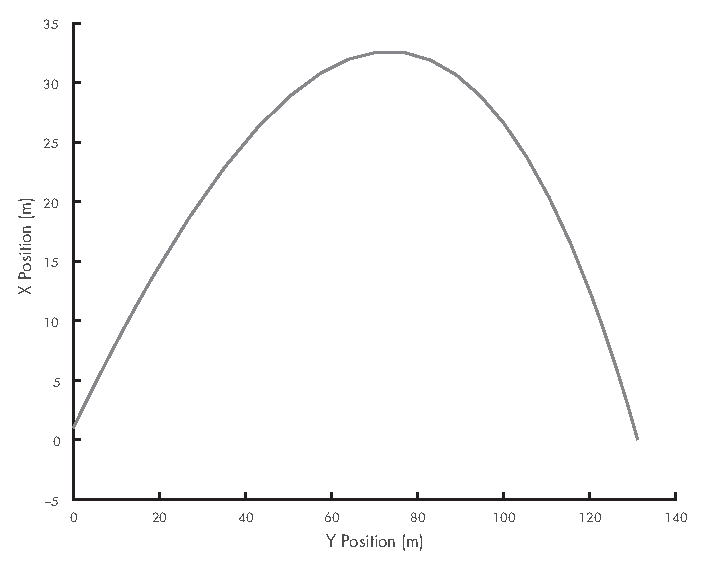
\includegraphics{book/images/figure13_01_new.eps}
\caption{Simulated flight of a baseball plotted as a trajectory}
\label{fig:baseball3}
\end{figure}

\index{trajectory}


\section{Range Versus Angle}

Now we'd like to simulate the trajectory of the baseball with a range of launch angles.  First, we'll take the code we have and wrap it in a function that takes the launch angle as an input variable, runs the simulation, and returns the distance the ball travels (Listing~\ref{lst:baseball_range}).

\index{range}
\index{launch angle}

\begin{lstlisting}[caption={A function that takes the launch angle of a baseball and returns the distance it travels}, label={lst:baseball_range}]
function res = baseball_range(theta)
    P = [0; 1];       
    v = 50;           
    [vx, vy] = pol2cart(theta, v);
    
    V = [vx; vy];     % initial velocity in m/s
    W = [P; V];       % initial condition
    
    tspan = [0 10];
    options = odeset('Events', @event_func);
    [T, M] = ode45(@rate_func, tspan, W, options);
    
    res = M(end, 1);
end
\end{lstlisting}

The launch angle, \lstinline{theta}, is in radians.  The magnitude of velocity, \lstinline{v}, is always \SI{50}{\meter\per\second}.  We use \lstinline{pol2cart} to convert the angle and magnitude (\emph{polar} coordinates) to Cartesian components, \lstinline{vx} and \lstinline{vy}.

\index{radian}
\index{pol2cart@\lstinline{pol2cart}}
\index{Cartesian coordinates}
\index{polar coordinates}

After running the simulation we extract the final $x$ position and return it as an output variable.  

We can run this function for a range of angles like this:

\begin{code}
    thetas = linspace(0, pi/2);
    for i = 1:length(thetas)
        ranges(i) = baseball_range(thetas(i));
    end
\end{code}
And then plot \lstinline{ranges} as a function of \lstinline{thetas}:

\begin{code}
    plot(thetas, ranges)
\end{code}

Figure~\ref{fig:baseball4} shows the result.  As expected, the ball does not travel far if it's hit nearly horizontal or vertical. 
The peak is apparently near \SI{0.7}{\radian}.

\begin{figure}[H]
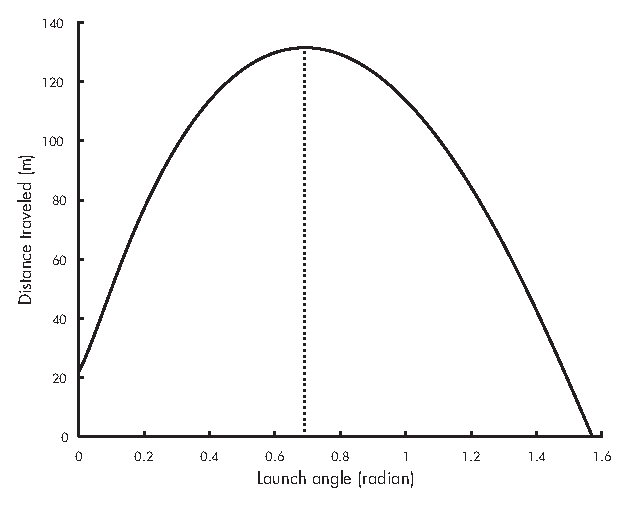
\includegraphics{book/images/figure13_02_new.eps}
\caption{Simulated flight of a baseball plotted as a trajectory}
\label{fig:baseball4}
\end{figure}


Considering that our model is only approximate, this result might be good enough.  But if we want to find the peak more precisely, we can use \lstinline{fminsearch}.


\section{fminsearch}

The \lstinline{fminsearch} function is similar to \lstinline{fzero}, which we saw in Chapter~\ref{fzero}.  Recall that \lstinline{fzero} takes a function handle and an initial guess, and returns a root of the function.
As an example, to find a root of this function:

\index{fminsearch@\lstinline{fminsearch}}
\index{fzero@\lstinline{fzero}}

\begin{code}
function res = error_func(x)
    res = x^2 - 2;
end
\end{code}
We can call \lstinline{fzero} like this:

\begin{code}
>> ***x = fzero(@error_func, 1)***
ans = 1.4142
\end{code}

The result is near the square root of 2.  If we call \lstinline{fminsearch} with the same function:

\begin{code}
>> ***x = fminsearch(@error_func, 1)***
x = -8.8818e-16
\end{code}

The result is close to 0, which is where this function is minimized.  Optionally, \lstinline{fminsearch} returns two values:

\begin{code}
>> ***[x, fval] = fminsearch(@error_func, 1)***
x = -8.8818e-16

fval = -2
\end{code}

The \lstinline{x} is the location of the minimum and \lstinline{fval} is the value of the function evaluated at \lstinline{x}.

If we want to find the maximum of a function, rather than the minimum, we can still use \lstinline{fminsearch} by writing a short function that negates the function we want to maximize.
In the baseball example, the function we want to maximize is \lstinline{baseball_range}; we can wrap it in another function like this:

\begin{code}
function res = min_func(angle)
    res = -baseball_range(angle);
end
\end{code}

And call \lstinline{fminsearch} like this:

\begin{code}
>> ***[x, fval] = fminsearch(@min_func, pi/4)***

x = 0.6921

fval = -131.5851
\end{code}

The optimal launch angle for the baseball is \SI{0.69}{\radian}; launched at that angle, the ball travels almost \SI{132}{\meter}.

If you're curious about how \lstinline{fminsearch} works, see ``\nameref{howfminsearch}'' on page~\pageref{howfminsearch}.


\section{Animation}

Animation is a useful tool for checking the results of a physical model.  
If something is wrong, animation can make it obvious.
There are two ways to do animation in MATLAB.  
One is to use \lstinline{getframe} to capture a series of images and \lstinline{movie} to play them back.

\index{animation}
\index{getframe@\lstinline{getframe}}

The more informal way is to draw a series of plots.  Listing~\ref{lst:animate} is a function that animates the results of a baseball simulation:

\begin{lstlisting}[caption={A function that animates the results of a baseball simulation}, label={lst:animate}]
function animate(T,M)
    X = M(:,1);
    Y = M(:,2);

    minmax = [min([X]), max([X]), min([Y]), max([Y])];

    for i=1:length(T)
        clf; hold on
        axis(minmax)
        plot(X(i), Y(i), 'o')
        drawnow;
        
        if i < length(T)
            dt = T(i+1) - T(i);
            pause(dt);
        end
    end
end
\end{lstlisting}

The input variables are the output from \lstinline{ode45}: \lstinline{T}, which contains the time values, and \lstinline{M}, which contains the position and velocity of the baseball.

\index{axis@\lstinline{axis}}

\lstinline{minmax} is a vector of four elements which is used inside the loop to set the axes of the figure.  
This is necessary because otherwise MATLAB scales the figure each time through the loop,
so the axes keep changing, which makes the animation hard to watch.

\index{clf@\lstinline{clf}}
\index{clear figure}

Each time through the loop, \lstinline{animate} uses \lstinline{clf}
to clear the figure and \lstinline{axis} to reset the axes.  Then it plots a circle to represent the position of the baseball.

\index{drawnow@\lstinline{drawnow}}

We have to call \lstinline{drawnow} after \lstinline{plot} so
that MATLAB actually displays each plot.  Otherwise it waits
until you finish drawing all the figures and then updates
the display.

We can call \lstinline{animate} like this:

\begin{code}
    tspan = [0 10];
    W = [0 1 30 40];
    [T, M] = ode45(@rate_func, tspan, W);
    animate(T, M)
\end{code}

One limitation of this kind of animation is that the speed
of the animation depends on how fast your computer can generate
the plots.  Since the results from \lstinline{ode45} are usually not
equally spaced in time, your animation might slow down where
\lstinline{ode45} takes small time steps and speed up where the time
step is larger.

\index{ode45@\lstinline{ode45}}
\index{time span}

One way to fix this problem is to change the way we specify \lstinline{tspan}.
Here's an example:

\begin{code}
    tspan = 0:0.1:10;
\end{code}

The result is a vector that goes from 0 to 10 with a step size of 0.1.  
Passing \lstinline{tspan} to \lstinline{ode45} in this form doesn't affect the accuracy of the results; 
\lstinline{ode45} still uses variable time steps to generate the estimates, but then it interpolates them before returning the results.

\index{step size}
\index{pause@\lstinline{pause}}

With equal time steps, the animation should be smoother.

Another option is to use \lstinline{pause} to play the animation in
real time.  After drawing each frame and calling
\lstinline{drawnow}, you can compute the time
until the next frame and use \lstinline{pause} to wait:

\begin{code}
    dt = T(i+1) - T(i);
    pause(dt);
\end{code}

A limitation of this method is that it ignores the time required to
draw the figure, so it tends to run slow, especially if the figure is
complex or the time step is small.

\section{Chapter Review}

This chapter presented two new tools, \lstinline{fminsearch} and \lstinline{animate}.  
The \lstinline{fminsearch} is a MATLAB function that searches efficiently for the minimum of a function, and can be adapted to search for the maximum, too.
The \lstinline{animate} is a function I wrote to read results from \lstinline{ode45} and generate an animation; the version in this chapter works with the results from the baseball simulation, but it can be adapted for other simulations.

In the exercises below, you have a chance to extend the example from this chapter and bring together many of the tools we have used so far.

In the next chapter, we move on to a new example, celestial mechanics, which describes the motion of planets and other bodies in outer space.


\section{Exercises}

Before you go on, you might want to work on the following exercises.

\subsection{Exercise 1}

\index{Manny Ramirez}
\index{Boston Red Sox}

Manny Ramirez is a former member of the Boston Red Sox who was famous for his relaxed attitude.  The goal of this exercise is to solve the following Manny-inspired problem:

\begin{quote}
What is the minimum effort required to hit a home run in Fenway Park?
\end{quote}

\index{Fenway Park}

Fenway Park is a baseball stadium in Boston, Massachusetts.  One of its most famous features is the ``Green Monster,'' which is a wall in left field that is unusually close to home plate, only 310 feet away.  To compensate for the short distance, the wall is unusually high, at 37 feet.

\index{Ramirez, Manny}
\index{Fenway Park}
\index{baseball}
\index{Green Monster}
\index{velocity}

You can solve this problem in two steps:

\begin{enumerate}

\item For a given velocity, find the launch angle that maximizes the height of the ball when it reaches the wall.  Notice that this is not quite the same as the angle that maximizes the distance the ball travels.

\index{launch angle}

\item Find the minimal velocity that clears the wall, given that it has the optimal launch angle.  Hint: this is actually a root-finding problem, not an optimization problem.

\end{enumerate}



\subsection{Exercise 2}
\label{golf}

\index{golf ball}
\index{force!Magnus}
\index{Magnus force}

A golf ball hit with backspin generates lift, which might increase the distance it travels, but the energy that goes into generating spin probably comes at the cost of lower initial velocity.

Write a simulation of the flight of a golf ball and use it to find
the launch angle and allocation of spin and initial velocity
(for a fixed energy budget) that maximizes the horizontal range of the
ball in the air.

The lift of a spinning ball is due to the Magnus force (see
\url{https://greenteapress.com/matlab/magnus}), which is
perpendicular to the axis of spin and the path of flight.  The
coefficient of lift is proportional to the spin rate; for a ball
spinning at 3000~rpm it is about 0.1.  The coefficient of drag of a
golf ball is about 0.2 as long as the ball is moving faster than \SI{20}{\meter\per\second}.





\chapter{Springs and Things}

The computational tools you have learned so far make up a versatile toolkit for modeling physicals systems described by first and second order differential equations and systems of equations.

With {\tt ode45} you can compute the state variables of these systems as they change over time.
By varying the parameters of the model, you can see what effect they have on the results.
Then you can use {\tt fminsearch} and {\tt fzero} to find minimums, maximums, and places where the outputs pass through zero.

These tools are all you need to solve a lot of problems, so this chapter doesn't present new computational tools (whew!).  Instead, we'll look at some different physical systems and some forces we haven't dealt with yet, including spring forces, electromagnetic forces, and univeral gravitation.

The examples in this chapter are a little more open ended than the previous ones.
I will present a motivating problem and some background information, and you will have a chance to implement the models as exercises.


\section{Bungee Jumping}
\label{bungee}

\index{bungee jump}
\index{cookie}
\index{tea}

Suppose you want to set the world record for the highest ``bungee dunk'', which is a stunt in which a bungee jumper dunks a cookie in a cup of tea at the lowest point of a jump.  An example is shown in this video: \emph{http://modsimpy.com/dunk}.

%TODO: Expand this URL or provide a new shortened URL.

Since the record is \SI{70}{\meter}, let's design a jump for \SI{80}{\meter}.  We'll start with the following parameters:

\begin{itemize}

\item  Initially the jumper stands on a platform \SI{80}{\meter} above a cup of tea.  One end of the bungee cord is connected to the platform, the other end is attached to the jumper, and the middle hangs down.

\item The mass of the jumper is \SI{75}{\kilogram}, and they are subject to gravitational acceleration of \SI{9.8}{\meter \per \second \squared}.

\item In free fall the jumper has a cross-sectional area of \SI{1}{\meter} and a terminal velocity of \SI{60}{\meter\per\second}.

\end{itemize}

To model the force of the bungee cord on the jumper, I'll make the following assumptions:

\begin{itemize}

\item Until the cord is fully extended, it applies no force to the jumper.  It turns out this might not be a good assumption; we'll revisit it in the next section.

\item After the cord is fully extended, it obeys Hooke's Law; that is, it applies a force to the jumper proportional to the extension of the cord beyond its resting length.

\end{itemize}

We can write Hooke's Law like this:

$F_s = -k x$

where $F_s$ is the force of the spring (bungee cord) on the jumper in Newtons, $x$ is the distance the spring is stretched by in meters, and $k$ is a spring constant that represents the strength of the spring in Newtons per meter.
The minus sign indicates that the spring force is opposite the direction the spring is stretched.

\index{Hooke's law}
\index{spring constant}

Hooke's Law is not a law in the sense that it is always true; really, it is a model of how some things behave under some conditions.
Almost everything obeys Hooke's Law when $x$ is small enough, but for large values everything deviates from this ideal behavior, one way or the other.

In reality, the spring constant of a bungee cord depends on $x$ over the range we are interested in, but as a starting place I'll assume $k$ is constant.



\begin{ex}

Write a simulation of this scenario, based on these parameters and modeling assumptions.
Use your simulation to choose the length of the cord, {\tt L}, and its spring constant, {\tt k}, so that the jumper falls all the way to the tea cup, but no farther!

You could start with the length \SI{25}{\meter} and spring constant \SI{40}{\newton \per \meter}.

\end{ex}


\section{Bungee Revisited}

\index{bungee jump}

In section, we modeled the motion of a bungee jumper taking into account gravity, air resistance, and the spring force of the bungee cord.  But we ignored the weight of the cord.

\index{bungee jump}
\index{bungee cord}

It's tempting to say that the cord has no effect because it falls along with the jumper, but that intuition is incorrect.  As the cord falls, it transfers energy to the jumper.

\index{acceleration}

At \emph{http://modsimpy.com/bungee} you'll find a paper by Heck, Uylings, and Kędzierska titled ``Understanding the physics of bungee jumping;" it explains this phenomenon and derives the acceleration of the jumper, $a$, as a function of position, $y$, and velocity, $v$:
%
\[ a = g + \frac{\mu v^2/2}{\mu(L+y) + 2L} \] 
%
where $g$ is acceleration due to gravity, $L$ is the length of the cord, and $\mu$ is the ratio of the mass of the cord, $m$, and the mass of the jumper, $M$.

If you don't believe that their model is correct, this video might convince you: \emph{http://modsimpy.com/drop}.

\begin{ex}

Modify your solution to the previous problem to model this effect.  How does the behavior of the system change as we vary the mass of the cord?  When the mass of the cord equals the mass of the jumper, what is the net effect on the lowest point in the jump?

\end{ex}


\section{Spider-Man}

In this case study we'll develop a model of Spider-Man swinging from a
springy cable of webbing attached to the top of the Empire State
Building.  Initially, Spider-Man is at the top of a nearby building, as
shown in Figure~\ref{spiderman}.

\index{Spider-Man}
\index{Empire State Building}

\begin{figure}
\centerline{\includegraphics[height=2.5in]{book/figs/spiderman.pdf}}
\caption{Diagram of the initial state for the Spider-Man case study.}
\label{spiderman}
\end{figure}

The origin, {\tt O}, is at the base of the Empire State Building. The
vector {\tt H} represents the position where the webbing is attached
to the building, relative to {\tt O}. The vector {\tt P} is the
position of Spider-Man relative to {\tt O}. And {\tt L} is the
vector from the attachment point to Spider-Man.

\index{vector addition}
\index{addition!vector}

By following the arrows from {\tt O}, along {\tt H}, and along
{\tt L}, we can see that

\begin{code}
H + L = P
\end{code}

So we can compute {\tt L} like this:

\begin{code}
L = P - H
\end{code}

The goals of this case study are:

\begin{enumerate}

\item
  Implement a model of this scenario to predict Spider-Man's trajectory.

\index{trajectory}

\item
  Choose the right time for Spider-Man to let go of the webbing in order
  to maximize the distance he travels before landing.

\index{range}

\item
  Choose the best angle for Spider-Man to jump off the building, and the best time to let go of the webbing, to maximize range.

\index{optimization}  
  
\end{enumerate}

We'll use the following parameters:

\index{parameter}

\begin{enumerate}

\item According to the Spider-Man Wiki (\emph{http://modsimpy.com/spider}), Spider-Man weighs \SI{76}{\kg}.

\item
  Let's assume his terminal velocity is \SI{60}{\meter\per\second}.

\index{terminal velocity}

\item
  The length of the web is \SI{100}{\meter}.

\item
  The initial angle of the web is \SI{45}{\degree} to the left of straight
  down.

\item
  The spring constant of the web is \SI{40}{\newton\per\meter} when the cord is stretched, and 0 when it's compressed.
  
\index{spring constant}

\end{enumerate}


\section{Celestial Mechanics}

\index{celestial mechanics}
\index{mechanics!celestial}

\emph{Celestial mechanics} describes how objects move in outer space.
If you did Exercise~\ref{earth}, you simulated the Earth being pulled toward the Sun in one dimension.  Now we'll simulate the Earth orbiting the Sun in two dimensions.

\index{Earth}
\index{Sun}

To keep things simple, we'll consider only the effect of the Sun on the Earth, and ignore the effect of the Earth on the Sun.  So we'll place the Sun at the origin and use a spatial vector, $\vec{P}$, to represent the position of the Earth relative to the Sun.

\index{position}
\index{spatial vector}
\index{mass}
\index{Law of universal gravitation}

Given the mass of the Sun, $m1$, and the mass of the Earth, $m2$, the gravitational force between them is

\begin{equation*}
\vec{F_g} = -G \frac{m_1 m_2}{r^2} \uvec{P}
\end{equation*}

where $G$ is the universal gravitational constant (see \emph{https://en.wikipedia.org/wiki/Gravity}),
$r$ is the distance of Earth from the Sun, and
$\uvec{P}$ is a unit vector in the direction of $\vec{P}$.

\index{universal gravitation constant}

\begin{ex}
Write a simulation of Earth orbiting the Sun.  You can look up the orbital velocity of the Earth, or search for the initial velocity that causes the earth to make one complete orbit in one year.  Optionally, use {\tt fminsearch} to find the velocity that gets the Earth as close as possible to the starting place after one year.

\index{velocity}
\index{fminsearch{\tt fminsearch}}

\end{ex}


\section{Conservation of Energy}

A useful way to check the accuracy of an ODE solver is to see whether it conserves energy.  For planetary motion, it turns out that {\tt ode45} does not.

\index{ode45@{\tt ode45}}
\index{conservation of energy}
\index{energy}
\index{kinetic energy}
\index{potential energy}

The kinetic energy of a moving body is

\begin{equation*}
KE = m v^2 / 2
\end{equation*}

The potential energy of a sun with mass $m_1$ and a
planet with mass $m_2$ and a distance $r$ between them is

\begin{equation}
PE = -G \frac{m_1 m_2}{r}
\end{equation}

Write a function called {\tt energy\_func} that takes the output of
your Earth simulation and computes the total
energy (kinetic and potential) of the system for each estimated
position and velocity.

Plot the result as a function of time and
check whether it increases or decreases over the course of the simulation.

\index{tolerance}
\index{odeset@{\tt odeset}}

You can reduce the rate of energy loss by decreasing {\tt ode45}'s
tolerance option using {\tt odeset} (see Section~\ref{events}):

\begin{code}
options = odeset('RelTol', 1e-5);
[T, M] = ode45(@rate_func, tspan, W, options);
\end{code}

The name of the option is {\tt RelTol} for ``relative tolerance.''
The default value is {\tt 1e-3} or 0.001.  Smaller values
make {\tt ode45} less ``tolerant'', so it does more work to
make the errors smaller.

\index{RelTol@{\tt RelTol}}

Run {\tt ode45} with a range of values for {\tt RelTol} and confirm
that as the tolerance gets smaller, the rate of energy loss
decreases.

\index{ode23@{\tt ode23}}

Along with {\tt ode45}, MATLAB provides several other ODE solvers 
(see \emph{https://www.mathworks.com/help/matlab/math/choose-an-ode-solver.html}).
Run your simulation with one of the other ODE solvers MATLAB provides
and see if any of them conserve energy.  You might find that {\tt ode23} works surprisingly well (although technically it does not conserve energy either).


\section{Cyclotron}

One of the most important inventions of the 20th Century is the cyclotron...

%TODO: Add this section



\printindex

\end{document}

